\باب{گھومتے مشین کے بنیادی اصول}
اس باب میں مختلف گھومتے مشینوں کے بنیادی اصولوں پر غور کیا جائے گا۔ظاہری طور پر مختلف مشین ایک ہی قسم کے اصولوں پر کام کرتے ہیں جنہیں اس باب میں اکٹھا کیا گیا ہے۔

\حصہ{قانون فیراڈے}
\اصطلاح{قانون فیراڈے}\فرہنگ{فیراڈے!قانون}\حاشیہب{Faraday's law}\فرہنگ{Faraday's law} کے تحت جب بھی کسی لچھے کا ارتباط بہاو  \عددیء{\lambda} وقت کے ساتھ تبدیل ہو، اس لچھے میں برقی دباو پیدا ہو گا:
\begin{align}
e=\frac{\partial \lambda}{\partial t}=N \frac{\partial \phi}{\partial t}
\end{align}
چونکہ ہمیں برقی دباو کی قیمت نا کہ اس کے \عددیء{\mp}  سے دلچسپی ہے لہٰذا اس مساوات میں منفی کی علامت کو نظر انداز کیا گیا ہے۔

گھومتے مشین میں ارتباط بہاو کی تبدیلی مختلف طریقوں سے پیدا کی جا سکتی ہے۔مثلاً  لچھے کو ساکن مقناطیسی بہاو میں گھما کر یا  ساکن لچھے میں مقناطیس گھما کر، وغیرہ وغیرہ۔

ان برقی مشینوں میں لچھے مقناطیسی قالب\فرہنگ{قالب}\حاشیہب{magnetic core}\فرہنگ{core}  پر لپیٹے جاتے ہیں۔ اس طرح کم سے کم مقناطیسی دباو سے زیادہ سے زیادہ مقناطیسی بہاو حاصل کیا جاتا ہے اور لچھوں کے مابین مشترکہ مقناطیسی بہاو بڑھایا جاتا ہے۔ مزید قالب کی شکل تبدیل کر کہ مقناطیسی بہاو کو ضرورت کے مقام پر پہنچایا جاتا ہے۔

ان مشینوں کے قالب میں مقناطیسی بہاو وقت کے ساتھ تبدیل ہوتا ہے لہٰذا قالب میں بھنور نما برقی رو\فرہنگ{بھنور نما برقی رو}\فرہنگ{برقی رو!بھنور نما}\حاشیہب{eddy currents}\فرہنگ{eddy currents} پیدا ہوتا ہے۔ان بھنور نما برقی رو کو کم سے کم کرنے کی خاطر  باریک لوہے کی پتری\فرہنگ{پتری}\حاشیہب{laminations}\فرہنگ{laminations} تہہ در تہہ رکھ قالب بنایا جاتا ہے ۔  آپ کو یاد ہو گا، ٹرانسفارمر کا قالب بھی اسی طرح بنایا جاتا ہے۔

\حصہ{معاصر مشین}
شکل \حوالہ{شکل_گھومتے_مشین_دو_قطب_ایک_دور_معاصر_بنیادی_شکل}  میں \اصطلاح{معاصر} برقی جنریٹر کا ایک بنیادی شکل دکھایا گیا ہے۔ اس کے قالب میں ایک مقناطیس ہے جو کہ گھوم سکتا ہے۔ مقناطیس کا مقام اس کے میکانی زاویہ \عددیء{\theta_m} سے بتلائی جاتی ہے۔ افقی لکیر سے گھڑی کے الٹ سمت زاویہ \عددیء{\theta_m} ناپا جاتا ہے۔

یہاں کچھ باتیں وضاحت طلب ہیں۔ اگر مقناطیس ایک مقررہ رفتار سے، فی سیکنڈ \عددیء{n}  مکمل چکر کاٹتا ہو تب ہم کہتے ہیں کہ اس مقناطیس کے گھومنے کا تعدد \عددیء{n}  ہرٹز\حاشیہب{Hertz} ہے۔اسی بات کو یوں بھی بیان کیا جاتا ہے کہ مقناطیس \عددیء{60n} چکر فی منٹ\فرہنگ{چکر فی منٹ}\حاشیہب{rounds per minute, rpm} کی رفتار سے گھوم رہا ہے۔ آپ جانتے ہیں کہ ایک چکر \عددیء{360\degree} زاویہ یا \عددیء{2 \pi} ریڈیئن\حاشیہب{radians}  پر مشتمل ہوتا ہے لہٰذا  گھومنے کی اس رفتار کو \عددیء{2\pi n} ریڈیئن فی سیکنڈ بھی کہہ سکتے ہیں۔ یوں اگر مقناطیس \عددیء{f} ہرٹز کی رفتار سے گھوم رہا ہو تب یہ \عددی{2\pi f} ریڈیئن فی سیکنڈ کی رفتار سے گھومے گا جس کو \عددی{\omega} سے ظاہر کیا جاتا ہے۔
\begin{align}
\omega =2\pi f
\end{align}
اس کتاب میں گھومنے کی رفتار کو عموماً ریڈیئن فی سیکنڈ میں بیان کیا جائے گا۔
\begin{figure}
\centering
%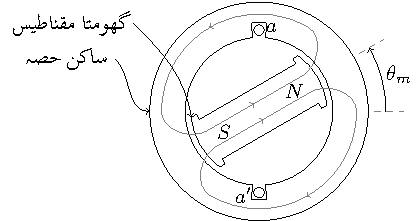
\includegraphics{figRotatingMachPrinciplesTwoPoleSinglePhaseSynchronousMachineBasic}
\begin{tikzpicture}
\stator{2}{90}
\rotor{2}{30}
%FLUX
\begin{scope}[rotate=30]
\pgfmathsetmacro{\delAngle}{30}   %smooth flux entry into stator
\draw[gray] (0,\rT/5)--++(0:0.8*\rR) to [out=0,in=-90+\delAngle] (\delAngle:\sRo-0.2) arc (\delAngle:180-\delAngle:\sRo-0.2)coordinate (leftUpperFlux);
\draw[gray,<-](0,\rT/5)--++(180:0.8*\rR) to [out=180,in=-90-\delAngle] (leftUpperFlux);
\draw[gray,->] (90-1:\sRo-0.2) to [out=180,in=0](90+1:\sRo-0.2);
\draw[gray] (0,-\rT/5)--++(0:0.8*\rR) to [out=0,in=90-\delAngle] (-\delAngle:\sRo-0.2) arc (-\delAngle:-180+\delAngle:\sRo-0.2)coordinate (leftLowerFlux);
\draw[gray,<-](0,-\rT/5)--++(180:0.8*\rR) to [out=180,in=90+\delAngle] (leftLowerFlux);
\draw[gray,->] (-90+1:\sRo-0.2) to [out=180,in=0](-90-1:\sRo-0.2);
\draw node at (0:0.6*\rR){$N$};
\draw node at (180:0.6*\rR){$S$};
\end{scope}
\slotEmptyCircle{90,-90}
\slotName{90/a/right,270/a'/left}
\draw [gray,dashed](0:\sRo+0.1)--++(0:0.5);
\draw [gray,dashed](30:\sRo+0.1)--++(30:0.5);
\draw[->] ([shift={(0:\sRo+0.3)}]0,0) arc (0:30:\sRo+0.3);
\draw node at (30/2:\sRo+0.6){$\theta_m$};
\draw node[left,->] at (160:1.4*\sRo){\RL{ساکن حصہ}};;
\draw[->] (160:1.4*\sRo) to [out=-45,in=180] (180:\sRo);
\draw node[left,->] at (145:1.4*\sRo){\RL{گھومتا مقناطیس}};;
\draw[->] (145:1.4*\sRo) to [out=-45,in=100] (185:\rR);
\end{tikzpicture}
\caption{دو قطب، ایک دور معاصر جنریٹر۔}
\label{شکل_گھومتے_مشین_دو_قطب_ایک_دور_معاصر_بنیادی_شکل}
\end{figure}

شکل \حوالہ{شکل_گھومتے_مشین_دو_قطب_ایک_دور_معاصر_بنیادی_شکل} میں  مشین کے دو مقناطیسی  قطب ہیں، اس لئے اس کو دو قطبی مشین کہتے ہیں۔ ساکن قالب میں، اندر کی جانب دو  شگاف ہیں، جن میں  \عددیء{N} چکر کا لچھا موجود ہے۔ لچھے کو \عددیء{a} اور \عددیء{a'} سے ظاہر کیا گیا ہے۔اس لچھے کی بنا اس مشین کو ایک لچھے کا مشین بھی کہتے ہیں۔ چونکہ یہ لچھا جنریٹر کے ساکن حصہ پر پایا جاتا ہے لہٰذا  یہ لچھا  بھی ساکن  ہو گا جس کی بنا اسے  \اصطلاح{ساکن لچھا}\فرہنگ{ساکن لچھا}\حاشیہب{stator coil}\فرہنگ{stator coil} کہتے ہیں۔

مقناطیس کا مقناطیسی بہاو شمالی قطب\حاشیہب{north pole}  \عددیء{N} سے خارج ہو کر خلائی درز میں سے ہوتا ہوا، باہر گول قالب میں سے گزر کر، دوسرے خلائی درز میں سے ہوتا ہوا، مقناطیس کے جنوبی قطب\حاشیہب{south pole}   \عددیء{S} میں داخل ہو گا۔ اس مقناطیسی بہاو کو  ہلکی سیاہی کے لکیروں سے دکھایا گیا ہے۔  یہ  مقناطیسی بہاو، سارا کا سارا، ساکن لچھے میں سے بھی گزرتا ہے۔شکل \حوالہ{شکل_گھومتے_مشین_دو_قطب_ایک_دور_معاصر_بنیادی_شکل}  میں مقناطیس سیدھی سلاخ کی مانند دکھایا گیا ہے۔

 شکل \حوالہ{شکل_گھومتے_مشین_رداس_اور_مقناطیسی_بہاو}  میں مقناطیس تقریباً گول ہے اور اس کے محور کا زاویہ \عددیء{\theta_m} صفر کے برابر ہے۔مقناطیس اور ساکن قالب کے بیچ صفر زاویہ،  \عددیء{\theta=0\degree} ، پر خلائی درز کی لمبائی کم سے کم اور نوے  زاویہ، \عددیء{\abs{\theta}=90\degree} ، پر زیادہ سے زیادہ ہے۔کم خلائی درز پر ہچکچاہٹ کم ہو گی جبکہ زیادہ خلائی درز  پر ہچکچاہٹ زیادہ ہو گی لہٰذا \عددی{\theta=0\degree} پر خلائی درز سے زیادہ مقناطیسی بہاو گزرے گا جبکہ \عددی{\theta=90\degree} پر کم بہاو گزرے گا۔خلائی درز کی لمبائی یوں تبدیل کی جاتی  ہے کہ  خلائی درز میں سائن نما مقناطیسی بہاو پیدا ہو۔ مقناطیسی بہاو مقناطیس سے قالب میں عمودی زاویہ پہ داخل ہوتا ہے۔  اگر خلائی درز میں \عددیء{B} سائن نما ہو
\begin{align}
B=B_0 \cos \theta_p
\end{align}
تب کثافت مقناطیسی بہاو \عددی{B} صفر زاویہ \عددیء{\theta_p=0\degree}، پر زیادہ سے زیادہ اور نوے زاویہ، \عددیء{\abs{\theta_p}=90\degree} ، پر صفر ہو گی اور خلائی درز میں مقناطیسی بہاو  \عددیء{\theta_p} کے ساتھ تبدیل ہو گا۔\عددیء{\theta_p} کو مقناطیس کے شمالی قطب  سے گھڑی کے مخالف رخ ناپا جاتا ہے۔  شکل \حوالہ{شکل_گھومتے_مشین_رداس_اور_مقناطیسی_بہاو}  میں  ساکن حصے کے باہر نوکیلی لکیروں کی لمبائی  سے  کثافت مقناطیسی بہاو کی مطلق قیمت اور لکیروں کے رخ سے بہاو کا رخ دکھایا گیا ہے۔اس شکل میں ہلکی سیاہی سے \عددیء{-40\degree}، \عددیء{60\degree} اور \عددیء{160\degree} زاویوں پر رداسی رخ  دکھایا گیا ہے۔زاویات \عددیء{-40\degree} اور  \عددیء{60\degree}  پر مقناطیسی بہاو رداسی رخ  جبکہ  \عددیء{160\degree} پر مقناطیسی بہاو رداسی رخ کے مخالف ہے۔یوں شکل \حوالہ{شکل_گھومتے_مشین_رداس_اور_مقناطیسی_بہاو} میں  آدھے خلائی درز میں کثافت مقناطیسی بہاو  رداسی رخ جبکہ باقی آدھے میں مخالف رداسی رخ ہو گا۔ خلائی درز میں کثافت مقناطیسی بہاو \عددیء{B} اور  \عددیء{\theta_p} کا ترسیم  سائن نما ہو گا۔ شکل \حوالہ{شکل_گھومتے_مشین_رداس_اور_مقناطیسی_بہاو_مقناطیس_گھوما_ہے}  میں مقناطیس دوسرے زاویہ پر دکھایا گیا ہے۔یاد رہے کثافت مقناطیسی بہاو کی مطلق قیمت  مقناطیس کے شمالی قطب پر زیادہ سے زیادہ ہو گی اور شمالی قطب پر کثافت مقناطیسی بہاو رداسی رخ ہو گی۔ شکل \حوالہ{شکل_گھومتے_مشین_رداس_اور_مقناطیسی_بہاو_مقناطیس_گھوما_ہے} میں خلائی درز میں کثافتِ مقناطیسی بہاو \عددیء{B}، زاویے \عددیء{\theta_p} اور \عددیء{\theta_m} دکھائے گئے ہیں جہاں سے درج ذیل لکھا جا سکتا ہے۔
\begin{gather}
\begin{aligned}\label{مساوات_گھومتے_مشین_کثافت_بالمقابل_میکانی_زاویہ}
B&=B_0 \cos \theta_p\\
\theta_p&=\theta-\theta_m
\end{aligned}
\end{gather}
یوں درج ذیل ہو گا۔
\begin{align}
B=B_0 \cos (\theta-\theta_m)
\end{align}
%
\begin{figure}
\centering
%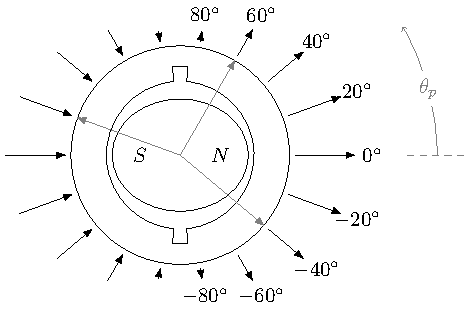
\includegraphics{figRotatingMachPrinciplesFluxVersusAngle}
\begin{tikzpicture}
%grid
%\draw[gray] (-\sRo,-\sRo) grid (\sRo,\sRo);
\stator{2}{90}
%elliptic rotor
\draw (-90:\rR-2*\gap) to [out=0,in=-90] (0:\rR) to [out=90,in=0] (90:\rR-2*\gap) to [out=180,in=90] (180:\rR) to [out=-90,in=180] (-90:\rR-2*\gap);
\draw node at (0:0.6*\rR){$N$};
\draw node at (180:0.6*\rR){$S$};
%flux
\foreach \angle in {-80,-60,...,80}{
\draw[-latex] (\angle:\sRo+\gap)--++(\angle:cos \angle) node[shift={(\angle:0.3)}] {$\angle\degree$};}
\foreach \angle in {100,120,...,260}{
\draw[latex-] (\angle:\sRo+\gap)--++(\angle:-cos \angle);}
%
\draw[gray,-latex] (0,0)--(-40:\sRo);
\draw[gray,-latex] (0,0)--(60:\sRo);
\draw[gray,-latex] (0,0)--(160:\sRo);
%
\draw[gray,dashed] (0:\sRo+2)--++(0:1);
\draw[gray,->] (0:\sRo+2.5) arc (0:30:\sRo+2.5);
\draw node[gray,fill=white] at (15:\sRo+2.5){$\theta_p$};
\end{tikzpicture}
\caption{کثافتِ مقناطیسی بہاو اور زاویہ کا تبدیلی۔}
\label{شکل_گھومتے_مشین_رداس_اور_مقناطیسی_بہاو}
\end{figure}

شکل  \حوالہ{شکل_گھومتے_مشین_رداس_اور_مقناطیسی_بہاو_مقناطیس_گھوما_ہے} میں مقناطیس اور اس کا سائن نما مقناطیسی دباو پیش کیا گیا ہے۔ جیسا شکل \حوالہ{شکل_گھومتے_مشین_مقناطیسی_دباو_سمتیہ}  میں دکھایا گیا ہے، ایسے مقناطیسی دباو کو عموماً ایک سمتیہ سے ظاہر کیا جاتا ہے جہاں سمتیہ کا طول مقناطیسی دباو کا حیطہ اور سمتیہ کا رخ مقناطیس کے شمال کو ظاہر کرتا ہے۔
\begin{figure}
\centering
%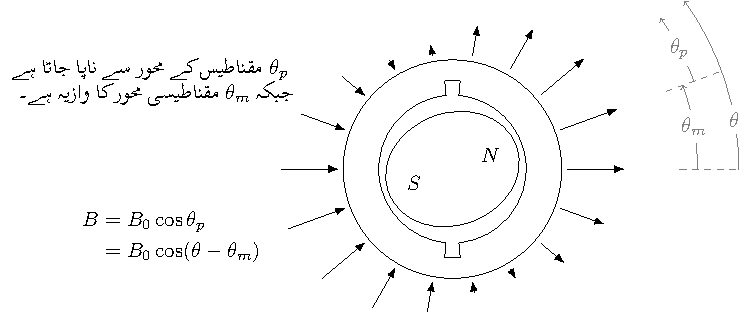
\includegraphics{figRotatingMachPrinciplesFluxVersusAngleTiltedRotor}
\begin{tikzpicture}
%grid
%\draw[gray] (-\sRo,-\sRo) grid (\sRo,\sRo);
\stator{2}{90}
%elliptic rotor
\begin{scope}[rotate=20]
\draw (-90:\rR-2*\gap) to [out=0,in=-90] (0:\rR) to [out=90,in=0] (90:\rR-2*\gap) to [out=180,in=90] (180:\rR) to [out=-90,in=180] (-90:\rR-2*\gap);
\draw node at (0:0.6*\rR){$N$};
\draw node at (180:0.6*\rR){$S$};
%flux
\foreach \angle in {-80,-60,...,80}{
\draw[-latex] (\angle:\sRo+\gap)--++(\angle:cos \angle) ;}
\foreach \angle in {100,120,...,260}{
\draw[latex-] (\angle:\sRo+\gap)--++(\angle:-cos \angle);}
%
\draw[gray,dashed] (0:\sRo+2)--++(0:1);
\draw[gray,->] (0:\sRo+2.5) arc (0:16:\sRo+2.5);
\draw node[gray,fill=white] at (8:\sRo+2.5){$\theta_p$};
\end{scope}
%
\draw[gray,dashed] (0:\sRo+2)--++(0:1);
\draw[gray,->] (0:\sRo+2.3) arc (0:20:\sRo+2.3);
\draw node[gray,fill=white] at (10:\sRo+2.3){$\theta_m$};
%
\draw[gray,dashed] (0:\sRo+2)--++(0:1);
\draw[gray,->] (0:\sRo+3) arc (0:36:\sRo+3);
\draw node[gray,fill=white] at (10:\sRo+3){$\theta$};
%text
\draw node[left,align=right] at (150:1.6*\sRo){\RL{ $\theta_p$ مقناطیس کے محور سے ناپا جاتا ہے}\\ \RL{اور $\theta_m$ مقناطیسی محور کا زاویہ ہے۔}};
\draw node[left] at (200:1.8*\sRo){$\begin{aligned}  B&=B_0 \cos \theta_p\\&=B_0 \cos (\theta-\theta_m)  \end{aligned}$};
\end{tikzpicture}
\caption{کثافت مقناطیسی بہاو اور مقناطیس کا زاویہ۔}
\label{شکل_گھومتے_مشین_رداس_اور_مقناطیسی_بہاو_مقناطیس_گھوما_ہے}
\end{figure}
%
\begin{figure}
\centering
%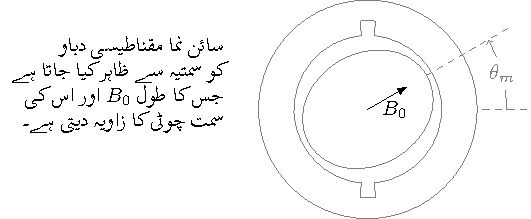
\includegraphics{figRotatingMachPrinciplesFluxVector}
\begin{tikzpicture}
%grid
%\draw[gray] (-\sRo,-\sRo) grid (\sRo,\sRo);
\begin{scope}[draw=gray]
\stator{2}{90}
\end{scope}
%elliptic rotor
\pgfmathsetmacro{\angle}{30}
\begin{scope}[rotate=\angle]
\draw[gray] (-90:\rR-2*\gap) to [out=0,in=-90] (0:\rR) to [out=90,in=0] (90:\rR-2*\gap) to [out=180,in=90] (180:\rR) to [out=-90,in=180] (-90:\rR-2*\gap);
%flux
\draw[-latex] (0,0) --(0:0.75)node [below,pos=0.7]{$B_0$};
\draw[gray,dashed] (0:\rR)--++(0:1.6);
\end{scope}
%
\draw[gray,dashed] (0:\sRo+0.1)--++(0:0.8);
\draw[gray,->] (0:\sRo+0.5) arc (0:\angle:\sRo+0.5);
\draw node[gray,fill=white] at (\angle/2:\sRo+0.5){$\theta_m$};
%text
\draw node[left,align=right] at (170:\sRo+0.5){\RL{سائن نما مقناطیسی دباو} \\  \RL{کو سمتیہ سے ظاہر کیا جاتا ہے} \\   \RL{جس کا  طول $B_0$ اور اس کا} \\  \RL{رخ چوٹی کا زاویہ دیتا ہے۔}}; 
\end{tikzpicture}
\caption{مقناطیسی دباو کو سمتیہ سے ظاہر کیا جاتا ہے۔}
\label{شکل_گھومتے_مشین_مقناطیسی_دباو_سمتیہ}
\end{figure}

 شکل \حوالہ{شکل_گھومتے_مشین_رداس_اور_مقناطیسی_بہاو_مقناطیس_گھوما_ہے}  میں مقناطیس کو لمحہ \عددیء{t_1}،  زاویہ \عددیء{\theta_m(t_1)} پر دکھایا گیا ہے جہاں ساکن لچھے کا ارتباط بہاو \عددیء{\lambda_\theta} ہے۔ اگر مقناطیس گھڑی کے مخالف رخ ایک مقررہ رفتار \عددیء{\omega_0} سے  گھوم رہا ہو تب ساکن لچھے میں اس لمحہ پر برقی دباو \عددیء{e(t)} پیدا ہو گا:
\begin{align}
e(t)=\frac{\dif \lambda_\theta}{\dif t}
\end{align}
آدھے چکر، \عددیء{\pi} ریڈیئن  گھومنے کے،  بعد  مقناطیسی  قطبین آپس میں جگہیں تبدیل کرتے ہیں، لچھے میں مقناطیسی بہاو کا رخ الٹ ہو گا،لچھے میں ارتباط بہاو \عددیء{-\lambda_\theta}  اور اس میں امالی برقی دباو \عددیء{-e(t)} ہو گا۔ایک مکمل چکر بعد مقناطیس  دوبارہ اسی مقام پر ہو گا جو شکل \حوالہ{شکل_گھومتے_مشین_رداس_اور_مقناطیسی_بہاو_مقناطیس_گھوما_ہے} میں دکھایا گیا ہے، ساکن لچھے کا ارتباط بہاو دوبارہ \عددیء{\lambda_\theta} اور اس میں امالی برقی دباو \عددیء{e(t)} ہو گا۔ یوں جب بھی مقناطیس  \عددیء{\theta_m=2\pi}  میکانی زاویہ طے کرے،  امالی برقی دباو کے  برقی زاویہ میں \عددیء{\theta_e=2\pi}  تبدیلی رونما ہو گی  لہٰذا دو قطب، ایک لچھے  کی مشین میں میکانی زاویہ \عددیء{\theta_m} اور برقی زاویہ \عددیء{\theta_e}  ایک دوسرے کے برابر ہوں گے:
\begin{align*}
\theta_e=\theta_m
\end{align*}
اس مشین میں اگر مقناطیس \عددیء{f_m} چکر فی سیکنڈ کی رفتار سے گھومتا ہو تب لچھے میں امالی برقی دباو \عددیء{e(t)} بھی ایک سیکنڈ میں \عددیء{f_m} مکمل چکر کاٹے گا لہٰذا  \عددیء{e(t)} کے \اصطلاح{تعدد}\فرہنگ{تعدد} \حاشیہب{frequency}\فرہنگ{frequency}\عددیء{f_e}   کی قیمت  \عددیء{f_m} ہرٹز\حاشیہب{Hertz} ہو گی۔
\begin{align*}
f_e=f_m
\end{align*}
%
\begin{figure}
\centering
%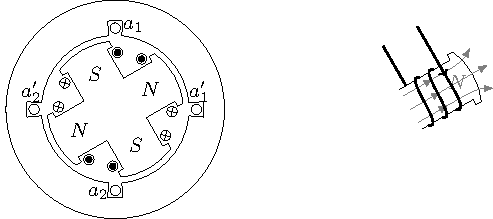
\includegraphics{figRotatingMachPrinciplesFourPoleFourSlotSynchronousMachine}
\begin{tikzpicture}
%grid
%\draw[gray] (-\sRo,-\sRo) grid (\sRo,\sRo);
\pgfmathsetmacro{\shiftX}{5cm}
\stator{4}{0}
\rotor{4}{30}

\slotEmptyCircle{0,90,180,270}
\slotName{0/a_1'/above,90/a_1/right,180/a_2'/above,270/a_2/left}
\dotCrossEachPole{30,210}
\crossDotEachPole{120,300}
\draw node at (30:0.6*\rR){$N$};
\draw node at (210:0.6*\rR){$N$};
\draw node at (120:0.6*\rR){$S$};
\draw node at (300:0.6*\rR){$S$};
%
\begin{scope}[xshift=\shiftX]
\pgfmathsetmacro{\rReduction}{0}   %reduction in rotor length due to adjacent rotor
\pgfmathsetmacro{\rWr}{1}    %rotor's flat section's effective length
\begin{scope}[rotate=30]
\draw(\rReduction,-\rT/2)--++(\rWr,0)--++(0,-\pY)--++(\pX,0)  arc (-\pTheta/2:\pTheta/2:\rR)--++(-\pX,0)--++(0,-\pY)--++(-\rWr,0);
\node[gray] at (0:0.8*\rR){$N$};
%flux
\draw[gray,-latex] (0,\rT/3)--++(0:0.5*\rR);
\draw[gray,-latex] (0,\rT/3)++(0:0.5*\rR)--++(0:0.3*\rR) to [out=0,in=210] (1.2*\rR,\rT/2);
\draw[gray,-latex] (0,0)--++(0:0.5*\rR);
\draw[gray,-latex] (0,0)++(0:0.5*\rR)--++(0:0.8*\rR);
\draw[gray,-latex] (0,-\rT/3)--++(0:0.5*\rR);
\draw[gray,-latex] (0,-\rT/3)++(0:0.5*\rR)--++(0:0.3*\rR) to [out=0,in=150] (1.2*\rR,-\rT/2);
\begin{scope}[rotate=-90]
%COIL
%left leg coil.  drawn from top to bottom
%======
\pgfmathsetmacro{\nL}{3}
\pgfmathsetmacro{\stepHL}{(\rWr-\pX-\gap)/(\nL)}
%
\def\leftEdge{-\rT/2};
\def\coilTop{\rWr-\pX-\gap};
\def\rightEdge{\rT/2};
%
\draw[thick](\leftEdge+\rT/4,\coilTop) to [out=0,in=45] (\rightEdge,{\coilTop-\stepHL/2}); %top half turn
%coil itself
\pgfmathsetmacro{\nLend}{\nL-2}
\foreach \y in { 0, ..., \nLend }{
\draw[thick] (\leftEdge,{\coilTop-\stepHL/2-\y*\stepHL}) to [out=-135,in=45] (\rightEdge,{\coilTop-\stepHL/2-\y*\stepHL-\stepHL});
} 
%left hand terminals
\draw[thick,<-] (\leftEdge+\rT/4,\coilTop)--++(-1.25*\rT,0) node(TA){};
\draw[thick] (\leftEdge,\coilTop-\nL*\stepHL+0.5*\stepHL)--++(-1*\rT,0)node(TB){};
%\node at ($(TA)!0.5!(TB)$){$\begin{aligned}&+\\ e&,\lambda\\&-   \end{aligned}$};
%=================================
\end{scope}
\end{scope}
\end{scope}
\end{tikzpicture}
\caption{چار قطب ایک دور معاصر جنریٹر۔}
\label{شکل_گھومتے_مشین_چار_قطب_معاصر_مژین}
\end{figure}


اس مشین میں  میکانی زاویہ \عددیء{\theta_m} اور برقی زاویہ \عددیء{\theta_e}  وقت کے ساتھ تبدیل ہونے کے باوجود آپس میں ایک تناسب رکھتے ہیں لہٰذا ایسے مشین کو \اصطلاح{معاصر} مشین\فرہنگ{معاصر}\حاشیہب{synchronous machine}\فرہنگ{synchronous}  کہتے ہیں۔ یہاں یہ تناسب ایک کے برابر ہے۔ 

شکل \حوالہ{شکل_گھومتے_مشین_چار_قطب_معاصر_مژین}  میں چار قطب، ایک دور معاصر جنریٹر دکھایا گیا ہے۔ چھوٹے مشینوں میں عموماً مقناطیس جبکہ بڑے مشینوں میں \اصطلاح{برقی مقناطیس}\فرہنگ{مقناطیس!برقی}\حاشیہب{electromagnet}\فرہنگ{electromagnet} استعمال ہوتے ہیں۔ اس شکل میں  برقی مقناطیس استعمال کیے گئے ہیں۔ دو سے زائد قطبین والے مشینوں میں کسی ایک شمالی قطب کو حوالہ قطب تصور کیا جاتا ہے۔ شکل میں اس حوالہ قطب کو \عددیء{\theta_m} پر دکھایا گیا ہے اور یوں دوسرا شمالی قطب \عددیء{(\theta_m+\pi)}  زاویہ پر ہے۔

 جیسا کہ نام سے واضح ہے، اس مشین میں  مقناطیس کے چار قطبین  ہیں۔ ہر ایک شمالی قطب کے بعد ایک جنوبی قطب آتا ہے۔ یک مرحلی آلات میں مقناطیسی  قطبین کے جوڑوں کی تعداد اور ساکن لچھوں کی تعداد ایک دوسرے کے برابر ہوتی ہے۔ شکل \حوالہ{شکل_گھومتے_مشین_چار_قطب_معاصر_مژین}  میں  مشین کے چار قطب یعنی دو جوڑی قطبین ہیں،  لہٰذا اس مشین کے ساکن حصہ پر دو ساکن لچھے ہوں ہیں۔ ایک لچھے کو \عددیء{a_1} سے واضح کیا گیا ہے اور دوسرے کو \عددیء{a_2} سے۔لچھے \عددیء{a_1} کو  قالب میں موجود دو شگاف \عددیء{a_1} اور \عددیء{a_1'} میں لپیٹا گیا ہے۔ اسی طرح \عددیء{a_2} لچھے کو دو شگاف \عددیء{a_2} اور \عددیء{a_2'} میں رکھا گیا ہے۔ ان دونوں لچھوں میں یکساں برقی دباو پیدا ہوتا ہے۔  دونوں لچھوں کو سلسلہ وار\حاشیہب{series connected} جوڑا جاتا ہے۔ اس طرح جنریٹر سے حاصل برقی دباو ایک لچھے میں پیدا  برقی دباو کا دگنا ہو گا۔ایک مرحلی آلات میں  قالب کو مقناطیس کے  قطبین کی تعداد کے برابر  حصوں میں تقسیم کرنے سے  مشین کا ہر ساکن لچھا ایک حصہ گھیرتا ہے۔ شکل \حوالہ{شکل_گھومتے_مشین_چار_قطب_معاصر_مژین} میں چار  قطبین  ہیں  لہٰذا اس کا ایک لچھا  نوے میکانی زاویہ کے احاطے کو گھیرتا ہے۔

ساکن اور حرکی لچھوں کی کارکردگی ایک دوسرے سے مختلف ہوتی ہے۔اس کی  وضاحت کرتے ہیں۔

جیسا پہلے بھی ذکر کیا گیا چھوٹی گھومتی مشینوں میں مقناطیسی میدان ایک مقناطیس  فراہم کرتا ہے جبکہ بڑی مشینوں میں برقی مقناطیس  میدان فراہم کرتا ہے۔اگرچہ اب تک کی اشکال میں مقناطیس کو گھومتا حصہ دکھایا گیا ہے، حقیقت میں مقناطیس  کسی مشین میں گھومتا اور کسی میں  ساکن ہو گا۔ میدان فراہم کرنے والا لچھا مشین کے کل برقی طاقت کے چند فی صد برابر برقی طاقت استعمال کرتا ہے۔میدان فراہم کرنے والے اس لچھے کو \اصطلاح{میدانی لچھا}\فرہنگ{لچھا!میدانی}\حاشیہب{field coil}\فرہنگ{field coil}  کہتے ہیں۔اس کے برعکس مشین میں موجود دوسری نوعیت کے لچھے کو \اصطلاح{قوی لچھا}\فرہنگ{لچھا!قوی}\حاشیہب{armature coil}\فرہنگ{armature coil}  کہتے ہیں۔برقی جنریٹر کے قوی لچھے سے  برقی طاقت  حاصل کی جاتی ہے ۔برقی موٹروں میں میدانی لچھے میں چند فی صد برقی طاقت کے ضیاع کے علاوہ  تمام برقی طاقت  قوی لچھے کو فراہم کی جاتی ہے۔
\begin{figure}
\centering
%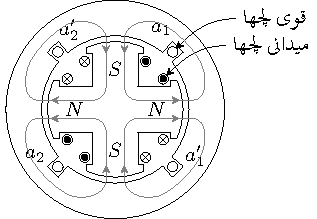
\includegraphics{figRotatingMachPrinciplesFourPoleTwoCoilFlux}
\begin{tikzpicture}
%grid
%\draw[gray] (-\sRo,-\sRo) grid (\sRo,\sRo);
\pgfmathsetmacro{\shiftX}{5cm}
\stator{4}{45}
\rotor{4}{0}

\slotEmptyCircle{45,135,-45,-135}
\dotCrossEachPole{0,180}
\crossDotEachPole{90,270}
\draw node at (0:0.6*\rR){$N$};
\draw node at (180:0.6*\rR){$N$};
\draw node at (90:0.6*\rR){$S$};
\draw node at (270:0.6*\rR){$S$};
%
%\slotName{45/a_1/,-45/a_1'/below,135/a_2'/,-135/a_2/below}
\draw (45+15:\sRi+1.25*\delR)node[]{$a_1$};
\draw (135-15:\sRi+1.25*\delR)node[]{$a_2'$};
\draw (-45+15:\sRi+1.25*\delR)node[]{$a_1'$};
\draw (-135-15:\sRi+1.25*\delR)node[]{$a_2$};
%text
\draw[stealth-] (45:\sRi cm+1/2*\delR cm+2.5pt) to [out=45,in=180] ++(1cm,0.5cm)node[right]{\RL{قوی لچھا}};
\draw[stealth-] (\rWf -\pX -1.3*\pX ,\rT/2 +1.3*\pX  )++(45:2.5pt) to [out=45,in=180] ++(1cm,0.5cm)node[right]{\RL{میدانی لچھا}};
%===========================
%FLUX 0degree to 90 degree
\pgfmathsetmacro{\delAngle}{30}   %smooth flux entry into stator
\draw[gray,-stealth] (\rT/2,\rT/5)coordinate(aa)--++(0:0.6*\rR);
\draw[gray](\rT/2,\rT/5)++(0:0.6*\rR)--++(0:0.2*\rR) to [out=0,in=-90+\delAngle] (\delAngle:\sRo-0.2) arc (\delAngle:90-\delAngle:\sRo-0.2)coordinate (leftUpperFlux);
\draw[gray] (\rT/5,\rT/2)coordinate(bb)--++(90:0.5*\rR);
\draw[gray,stealth-](\rT/5,\rT/2)++(90:0.5*\rR)--++(90:0.2*\rR) to [out=90,in=180-\delAngle] (leftUpperFlux);
\draw[gray] (bb) to [out=-90,in=180] (aa);
%====
%FLUX 0 degree to -90 degree
\draw[gray,-stealth] (\rT/2,-\rT/5)coordinate(aa)--++(0:0.6*\rR);
\draw[gray](\rT/2,-\rT/5)++(0:0.6*\rR)--++(0:0.2*\rR) to [out=0,in=90-\delAngle] (-\delAngle:\sRo-0.2) arc (-\delAngle:-90+\delAngle:\sRo-0.2)coordinate (leftUpperFlux);
\draw[gray] (\rT/5,-\rT/2)coordinate(bb)--++(-90:0.5*\rR);
\draw[gray,stealth-](\rT/5,-\rT/2)++(-90:0.5*\rR)--++(-90:0.2*\rR) to [out=-90,in=180+\delAngle] (leftUpperFlux);
\draw[gray] (bb) to [out=90,in=180] (aa);
%====
%FLUX 90 degree to 180 degree
\draw[gray,-stealth] (-\rT/2,\rT/5)coordinate(aa)--++(180:0.6*\rR);
\draw[gray](-\rT/2,\rT/5)++(180:0.6*\rR)--++(180:0.2*\rR) to [out=180,in=-90-\delAngle] (180-\delAngle:\sRo-0.2) arc (180-\delAngle:90+\delAngle:\sRo-0.2)coordinate (leftUpperFlux);
\draw[gray] (-\rT/5,\rT/2)coordinate(bb)--++(90:0.5*\rR);
\draw[gray,stealth-](-\rT/5,\rT/2)++(90:0.5*\rR)--++(90:0.2*\rR) to [out=90,in=\delAngle] (leftUpperFlux);
\draw[gray] (bb) to [out=-90,in=0] (aa);
%====
%FLUX -90 degree to 180 degree
\draw[gray,-stealth] (-\rT/2,-\rT/5)coordinate(aa)--++(180:0.6*\rR);
\draw[gray](-\rT/2,-\rT/5)++(180:0.6*\rR)--++(180:0.2*\rR) to [out=180,in=90+\delAngle] (180+\delAngle:\sRo-0.2) arc (180+\delAngle:270-\delAngle:\sRo-0.2)coordinate (leftUpperFlux);
\draw[gray] (-\rT/5,-\rT/2)coordinate(bb)--++(-90:0.5*\rR);
\draw[gray,stealth-](-\rT/5,-\rT/2)++(-90:0.5*\rR)--++(-90:0.2*\rR) to [out=-90,in=-\delAngle] (leftUpperFlux);
\draw[gray] (bb) to [out=90,in=0] (aa);
\end{tikzpicture}
\caption{چار قطب، دو لچھے مشین میں مقناطیسی بہاو۔}
\label{شکل_گھومتے_مشین_چار_قطب_کا_بہاو}
\end{figure}

%%%%%%%%%%%%%%%%%%%%%%%%%%%

اب اگر ہم، گھومتے اور ساکن حصہ کے درمیان، خلائی درز میں \عددیء{B} کو دیکھیں تو شمالی قطب سے مقناطیسی بہاو باہر کی جانب  نکل کر  قالب میں داخل ہوتا ہے جبکہ جنوبی قطب میں مقناطیسی بہاو قالب سے نکل کر جنوبی قطب میں اندر کی جانب داخل ہوتا ہے۔ یہ شکل \حوالہ{شکل_گھومتے_مشین_چار_قطب_کا_بہاو}  میں دکھایا گیا ہے۔ یوں اگر ہم اس خلائی درز میں ایک گول چکر کاٹیں تو مقناطیسی بہاو کی سمت  دو مرتبہ باہر کی جانب اور دو مرتبہ اندر کی جانب ہو گی۔ مزید یہ کہ   آلوں میں کوشش کی جاتی ہے کہ خلائی درز میں \عددیء{B} سائن نما ہو۔ یہ کیسے کیا جاتا ہے، اس کو ہم آگے پڑھیں گے۔  لہٰذا اگر یہ تصور کر لیا جائے کہ \عددیء{B} سائن نما ہی ہے تب  خلائی درز میں \عددیء{B} کی مقدار، شکل \حوالہ{شکل_گھومتے_مشین_سائن_نما_بہاو}  کی طرح ہو گی۔اس شکل میں برقی زاویہ \عددیء{\theta_e} استعمال کیا گیا ہے۔ 
\begin{figure}
\centering
%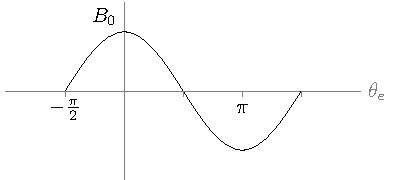
\includegraphics{figRotatingMachPrinciplesCosineFlux}
\begin{tikzpicture}
%grid
%\draw[gray] (-\sRo,-\sRo) grid (\sRo,\sRo);
\draw[gray](-2,0) --(4,0)node[right]{$\theta_e$}; %axis
\draw[gray] (0,-1.5)--(0,1.5);
\draw[above left] node at (0,1){$B_0$};
\draw (0,1) cos (-1,0) node[below]{$-\tfrac{\pi}{2}$};
\draw (0,1) cos (1,0);
\draw (2,-1) cos (1,0);
\draw (2,-1) cos (3,0);
\foreach \x in {-1,1,2,3}{
\draw[gray](\x,0)--++(0,-0.1);}
\draw[gray](2,0)--++(0,-0.1)node[below,text=black]{$\pi$};
\end{tikzpicture}
\caption{سائن نما کثافتِ مقناطیسی بہاو۔}
\label{شکل_گھومتے_مشین_سائن_نما_بہاو}
\end{figure}

 یوں ہم ایک ایسی معاصر مشین جس میں \عددیء{P} قطب مقناطیس پایا جاتا ہو کے لئے لکھ سکتے ہیں
\begin{align}
\theta_e&=\frac{P}{2} \theta_m\\
f_e&=\frac{P}{2} f_m  \label{مساوات_گھومتے_مشین_برقی_میکانی_تعدد_تعلق}
\end{align}
اس صورت میں میکانی اور برقی تعدد ایک مرتبہ پھر آپس میں ایک نسبت رکتے ہیں۔ 
%
\ابتدا{مثال}
پاکستان میں گھروں اور کارخانوں میں \عددیء{\SI{50}{\hertz}} کی برقی طاقت فراہم کی جاتی ہے یعنی ہمارے ہاں \عددیء{f_e=50} ہے۔
\begin{itemize}
\item
اگر یہ برقی طاقت دو قطب کے جنریٹر سے حاصل کی جائے تو یہ جنریٹر  کس رفتار سے گھمایا جائے گا۔
\item
اگر جنریٹر کے بیس قطب ہوں تب یہ جنریٹر کس رفتار سے گھمایا جائے گا۔
\end{itemize}

حل:
\begin{itemize}
\item
مساوات \حوالہ{مساوات_گھومتے_مشین_برقی_میکانی_تعدد_تعلق}  سے ہم دیکھتے ہیں کہ اگر یہ برقی طاقت دو قطب،\عددیء{P=2}،  والے جنریٹر سے حاصل کی جائے تو اس جنریٹر کو \عددیء{f_m=50} چکر فی سیکنڈ یعنی \عددیء{3000} چکر فی منٹ\حاشیہب{rpm, rounds per minute} گھمانا ہو گا۔
\item
 اگر یہی برقی طاقت بیس قطب، \عددیء{P=20}،  والے جنریٹر سے حاصل کی جائے تو پھر اس جنریٹر کو \عددیء{f_m=5} چکر فی سیکنڈ یعنی \عددیء{300} چکر فی منٹ کی رفتار سے گھمانا ہو گا۔
\end{itemize}
\انتہا{مثال}
%

 اب یہ فیصلہ کس طرح کیا جائے کہ جنریٹر کے قطب کتنے رکھے جائیں۔ درحقیقت پانی سے چلنے والے جنریٹر سست رفتار جبکہ ٹربائن سے چلنے والے جنریٹر تیز رفتار ہوتے ہیں، لہٰذا پانی سے چلنے والے جنریٹر زیادہ قطب رکھتے ہیں جبکہ ٹربائن سے چلنے والے جنریٹر آپ کو دو قطب کے ہی ملیں گے۔
\begin{figure}
\centering
%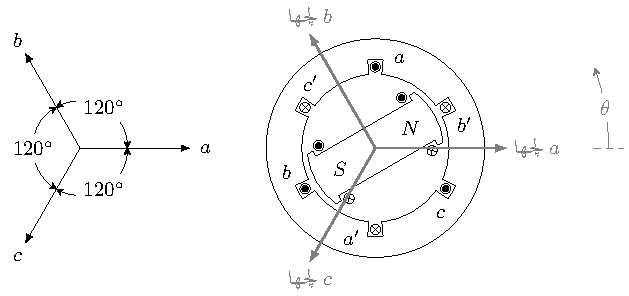
\includegraphics{figRotatingMachPrinciplesTwoPoleThreePhase}
\begin{tikzpicture}
%grid
%\draw[gray] (-\sRo,-\sRo) grid (\sRo,\sRo);
\pgfmathsetmacro{\shiftX}{5cm}
\stator{6}{30}
\slotDot{90,-30,210}
\slotCross{-90,30,150}
\rotor{2}{30}
\dotCrossEachPole{30}
\crossDotEachPole{210}
\draw node at (30:0.6*\rR){$N$};
\draw node at (210:0.6*\rR){$S$};
%
%\slotName{45/a_1/,-45/a_1'/below,135/a_2'/,-135/a_2/below}
\draw (90-15:\sRi+1.25*\delR)node[]{$a$};
\draw (270-15:\sRi+1.25*\delR)node[]{$a'$};
\draw (210-15:\sRi+1.25*\delR)node[]{$b$};
\draw (30-15:\sRi+1.25*\delR)node[]{$b'$};
\draw (-30-15:\sRi+1.25*\delR)node[]{$c$};
\draw (150-15:\sRi+1.25*\delR)node[]{$c'$};
%
\draw[thick,gray,-latex](0,0)--(0:1.2*\sRo)node[right]{\RL{$a$ لچھا}};
\draw[thick,gray,-latex](0,0)--(120:1.2*\sRo)node[above]{\RL{$b$ لچھا}};
\draw[thick,gray,-latex](0,0)--(-120:1.2*\sRo)node[below]{\RL{$c$ لچھا}};
%text
\draw[thin,gray,dashed] (0:2*\sRo)--++(0.25,0)coordinate(zeroAngle)--++(0.25,0);
\draw[gray,-stealth] (zeroAngle) arc (0:20:2*\sRo+0.25);
\node[fill=white,text=gray] at (10:2*\sRo+0.25){$\theta$};
%=============
\begin{scope}[xshift=-\shiftX]
\draw[-latex](0,0)--(0:1*\sRo)node[shift={(0:1*\sRo+0.2cm)}]{$a$};
\draw[-latex](0,0)--(120:1*\sRo)node[shift={(120:1*\sRo+0.2cm)}]{$b$};
\draw[-latex](0,0)--(-120:1*\sRo)node[shift={(-120:1*\sRo+0.2cm)}]{$c$};
%
\draw[stealth-stealth]([shift={(0:0.8)}]0,0)  arc (0:120:0.8);
\draw node at (60:0.8)[fill=white]{$120\degree$};
\draw[stealth-stealth]([shift={(0:0.8)}]0,0)  arc (0:-120:0.8);
\draw node at (-60:0.8)[fill=white]{$120\degree$};
\draw[stealth-stealth]([shift={(120:0.8)}]0,0)  arc (120:240:0.8);
\draw node at (180:0.8)[fill=white]{$120\degree$};
\end{scope}
\end{tikzpicture}
\caption{دو قطب، تین دور معاصر مشین۔}
\label{شکل_گھومتے_مشین_دو_قطب_تین_دور_معاصر}
\end{figure}

شکل \حوالہ{شکل_گھومتے_مشین_دو_قطب_تین_دور_معاصر}  میں دو قطب والا تین دور کا معاصر مشین دکھایا گیا ہے۔اس میں تین ساکن لچھے ہیں۔ان میں ایک لچھا \عددیء{a} ہے جو قالب میں  شگاف  \عددیء{a} اور \عددیء{a'} میں رکھا گیا ہے۔ اگر اس شکل میں باقی دو لچھے نہ ہوتے تو یہ بالکل شکل \حوالہ{شکل_گھومتے_مشین_دو_قطب_ایک_دور_معاصر_بنیادی_شکل}  میں دیا گیا مشین ہی تھا۔البتہ دیئے گئے شکل میں ایک کی بجائے تین ساکن لچھے ہیں۔

 اگر \عددیء{a} لچھا  میں برقی رو یوں ہو کہ شگاف \عددیء{a} میں برقی رو ، کتاب کے صفحہ سے عمودی رُخ میں باہر کی جانب ہو اور  \عددیء{a'} میں برقی رو کا رخ اس کے بالکل الٹ سمت میں ہو تو ہم لچھے کی سمت\فرہنگ{لچھا!سمت} کا تعین دائیں ہاتھ کے ذریعہ یوں کرتے ہیں۔

\begin{itemize}
\item
اگر ہم دائیں ہاتھ کی چار انگلیوں کو دونوں شگافوں میں برقی رو کی جانب لپٹیں تو اسی ہاتھ کا انگوٹھا لچھے کی سمت متعین کرتا ہے۔
\end{itemize}

 شکل \حوالہ{شکل_گھومتے_مشین_دو_قطب_تین_دور_معاصر}  میں لچھا \عددیء{a} کی سمت تیر والی لکیر سے دکھائی گئی ہے۔ اس سمت کو ہم صفر زاویہ تصور کرتے ہیں۔ لہٰذا شکل میں \عددیء{a} لچھا صفر زاویہ پر لپٹا گیا ہے، یعنی \عددیء{\theta_a=0\degree} ہے۔ باقی لچھوں کے زاویہ ، لچھا \عددیء{a} کی سمت سے، گھڑی کی اُلٹی رُخ، ناپے جاتے ہیں۔

شکل \حوالہ{شکل_گھومتے_مشین_دو_قطب_تین_دور_معاصر}  میں لچھا \عددیء{b} کو شگاف \عددیء{b} اور \عددیء{b'} میں رکھا گیا ہے اور لچھا \عددیء{c} کو شگاف \عددیء{c} اور \عددیء{c'} میں رکھا گیا ہے۔ مزید یہ کہ لچھا \عددیء{b} کو \عددیء{120\degree} کے زاویہ پر اور لچھا \عددیء{c} کو \عددیء{240\degree} زاویہ پر رکھا گیا ہے۔ یعنی \عددیء{\theta_b=120\degree} اور \عددیء{\theta_c=240\degree} ہیں۔
\begin{figure}
\centering
%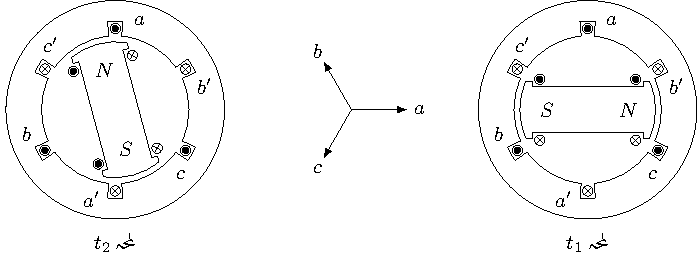
\includegraphics{figRotatingMachPrinciplesTwoPoleThreePhaseTwoMoments}
\begin{tikzpicture}
%grid
%\draw[gray] (-\sRo,-\sRo) grid (\sRo,\sRo);
\pgfmathsetmacro{\shiftX}{5cm}
\begin{scope}[xshift=0.8*\shiftX]
\stator{6}{30}
\slotDot{90,-30,210}
\slotCross{-90,30,150}
\rotor{2}{0}
\dotCrossEachPole{00}
\crossDotEachPole{180}
\draw node at (0:0.6*\rR){$N$};
\draw node at (180:0.6*\rR){$S$};
%
%\slotName{45/a_1/,-45/a_1'/below,135/a_2'/,-135/a_2/below}
\draw (90-15:\sRi+1.25*\delR)node[]{$a$};
\draw (270-15:\sRi+1.25*\delR)node[]{$a'$};
\draw (210-15:\sRi+1.25*\delR)node[]{$b$};
\draw (30-15:\sRi+1.25*\delR)node[]{$b'$};
\draw (-30-15:\sRi+1.25*\delR)node[]{$c$};
\draw (150-15:\sRi+1.25*\delR)node[]{$c'$};
%text
\node at (-90:\sRo+0.4){\RL{لمحہ $t_1$}};
\end{scope}
%=============
%\begin{scope}[xshift=-\shiftX]
\draw[-latex](0,0)--(0:0.5*\sRo)node[shift={(0:0.5*\sRo+0.2cm)}]{$a$};
\draw[-latex](0,0)--(120:0.5*\sRo)node[shift={(120:0.5*\sRo+0.2cm)}]{$b$};
\draw[-latex](0,0)--(-120:0.5*\sRo)node[shift={(-120:0.5*\sRo+0.2cm)}]{$c$};
%\end{scope}
%================
\begin{scope}[xshift=-0.8*\shiftX]
\stator{6}{30}
\slotDot{90,-30,210}
\slotCross{-90,30,150}
\rotor{2}{105}
\dotCrossEachPole{105}
\crossDotEachPole{285}
\draw node at (105:0.6*\rR){$N$};
\draw node at (285:0.6*\rR){$S$};
%
%\slotName{45/a_1/,-45/a_1'/below,135/a_2'/,-135/a_2/below}
\draw (90-15:\sRi+1.25*\delR)node[]{$a$};
\draw (270-15:\sRi+1.25*\delR)node[]{$a'$};
\draw (210-15:\sRi+1.25*\delR)node[]{$b$};
\draw (30-15:\sRi+1.25*\delR)node[]{$b'$};
\draw (-30-15:\sRi+1.25*\delR)node[]{$c$};
\draw (150-15:\sRi+1.25*\delR)node[]{$c'$};
%text
\node at (-90:\sRo+0.4){\RL{لمحہ $t_2$}};
\end{scope}
\end{tikzpicture}%
\caption{دو قطب تین دور مشین۔}
\label{شکل_گھومتے_مشین_دو_قطب_تین_دور_مختلف_لمحات}
\end{figure}

 شکل \حوالہ{شکل_گھومتے_مشین_دو_قطب_تین_دور_مختلف_لمحات}  میں دکھائے گئے لمحہ \عددیء{t_1} پر  اگر لچھے \عددیء{a} کا  ارتباط بہاو \عددیء{\lambda_a(t_1)} ہو تو جب مقناطیس \عددیء{120\degree} کا زاویہ طے کر لے، اس لمحہ \عددیء{t_2} پر  لچھے \عددیء{b} کا ارتباط بہاو \عددیء{\lambda_b(t_2)} ہو گا۔ ہم  دیکھتے ہیں کہ لمحہ \عددیء{t_2} پر مقناطیس اور لچھا \عددیء{b} آپس میں بالکل اسی طرح سے ہیں جیسے \عددیء{t_1} پر مقناطیس اور لچھا \عددیء{a} تھے۔ لہٰذا لمحہ \عددیء{t_2} پر لچھا \عددیء{b} کا ارتباط بہاو بالکل اتنا ہی ہو گا جتنا لمحہ \عددیء{t_1} پر  \عددیء{a} لچھا کا تھا۔ یعنی
\begin{align}
\lambda_b(t_2)=\lambda_a(t_1)
\end{align}
اسی طرح اگر مقناطیس مزید  \عددیء{120\degree} زاویہ طے کرے تو اس لمحہ \عددیء{t_3} پر لچھا \عددیء{c} کا ارتباط بہاو  \عددیء{\lambda_c(t_3)} ہو گا اور مزید یہ کہ یہ \عددیء{\lambda_a(t_1)} کے برابر ہو گا۔یوں
\begin{align}\label{مساوات_گھومتے_مشین_مختلف_اوقات_پر_تین_لچھے_یکساں}
\lambda_c(t_3)=\lambda_b(t_2)=\lambda_a(t_1)
\end{align}
ہیں۔ان لمحات پر ان  لچھوں میں
\begin{align}
e_a(t_1)&=\frac{\dif \lambda_a(t_1)}{\dif t}\\
e_b(t_2)&=\frac{\dif \lambda_b(t_2)}{\dif t}\\
e_c(t_3)&=\frac{\dif \lambda_c(t_3)}{\dif t}
\end{align}
ہوں گے۔مساوات \حوالہ{مساوات_گھومتے_مشین_مختلف_اوقات_پر_تین_لچھے_یکساں}    کی روشنی میں
\begin{align}\label{مساوات_گھومتے_مشین_تین_لمحات_دباو_یکساں}
e_a(t_1)=e_b(t_2)=e_c(t_3)
\end{align} 

اگر شکل \حوالہ{شکل_گھومتے_مشین_دو_قطب_تین_دور_مختلف_لمحات} میں صرف لچھا \عددیء{a} پایا جاتا تو یہ بالکل شکل \حوالہ{شکل_گھومتے_مشین_دو_قطب_ایک_دور_معاصر_بنیادی_شکل}   کی طرح ہوتا اور اب اگر اس میں مقناطیس کو گھڑی کی اُلٹی سمت ایک مقررہ رفتار \عددیء{\omega_0} سے گھمایا جاتا تو، جیسے پہلے تذکرہ کیا گیا ہے، لچھے \عددیء{a} میں سائن نما برقی دباو پیدا ہوتی۔شکل \حوالہ{شکل_گھومتے_مشین_دو_قطب_تین_دور_مختلف_لمحات}  میں کسی ایک لچھے کو کسی دوسرے لچھے پر کوئی برتری حاصل نہیں۔ لہٰذا اب شکل \حوالہ{شکل_گھومتے_مشین_دو_قطب_تین_دور_مختلف_لمحات}  میں اگر مقناطیس اسی طرح گھمایا جائے تو اس میں موجود تینوں ساکن لچھوں میں سائن نما برقی دباو پیدا ہو گی البتہ مساوات \حوالہ{مساوات_گھومتے_مشین_تین_لمحات_دباو_یکساں}    کے تحت یہ برقی دباو آپس میں  \عددیء{120\degree} کے زاویہ پر ہوں گے۔


\begin{figure}
\centering
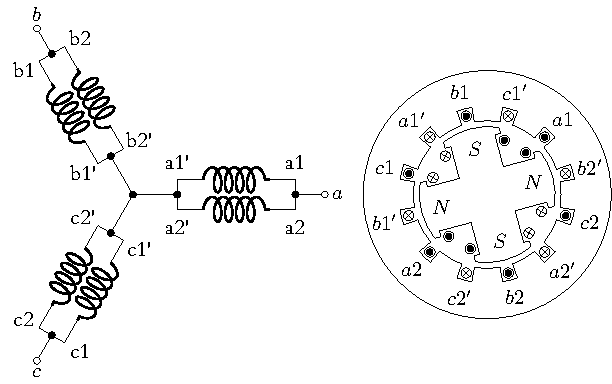
\includegraphics{figRotatingMachPrinciplesThreePhaseFourPole}
\caption{چار قطب، تین دور معاصر مشین۔}
\label{شکل_گھومتے_مشین_چار_قطب_تین_دور_معاصر}
\end{figure}
شکل \حوالہ{شکل_گھومتے_مشین_چار_قطب_تین_دور_معاصر} میں چار قطب، تین دور معاصر مشین دکھایا گیا ہے۔گھومتے حصے پر شمال اور جنوبی قطب باری باری پائے جاتے ہیں۔یوں شمال اور جنوب قطب کی ایک جوڑی \عددیء{180\degree} میکانی زاویہ طے کرتے ہیں۔یہی \عددیء{360\degree} برقی زاویہ بنتا ہے۔جیسا شکل \حوالہ{شکل_گھومتے_مشین_دو_قطب_تین_دور_معاصر} سے ظاہر ہے کہ ساکن حصے کے \عددیء{360\degree} برقی زاویہ پر تین دور کے لچھے نسب کئے جاتے ہیں۔یوں شکل \حوالہ{شکل_گھومتے_مشین_دو_قطب_تین_دور_معاصر} میں گھری کی الٹی سمت میں  \عددیء{a}، \عددیء{c'}، \عددیء{b}، \عددیء{a'}، \عددیء{c} اور \عددیء{b'} اسی ترتیب سے پائے جاتے ہیں۔شکل \حوالہ{شکل_گھومتے_مشین_چار_قطب_تین_دور_معاصر} میں  دو قطبین کے احاطے یعنی \عددیء{180\degree} میکانی زاویہ میں آپ کو بالکل اسی طرح تین دور کے  \عددیء{a1}، \عددیء{c1'}، \عددیء{b1}، \عددیء{a1'}، \عددیء{c1} اور \عددیء{c1'} نظر آتے ہیں۔بقایا دو قطبین کے احاطے میں بھی بالکل اسی طرح آپ کو \عددیء{a2}، \عددیء{c2'}، \عددیء{b2}،\عددیء{a2'}، \عددیء{c2} اور \عددیء{c2'} نظر آتے ہیں۔کسی بھی لمحہ \عددیء{a1} اور \عددیء{a2} لچھوں میں بالکل یکساں برقی دباو پیدا ہو گی۔تین دور کے دو یکساں لچھوں کو سلسلہ وار یا متوازی جوڑ کر تین دور کی برقی دباو حاصل کی جاتی ہے۔شکل میں انہیں متوازی جوڑ کر دکھایا گیا ہے جہاں \عددیء{a} لچھے کو صفر زاویہ پر تصور کیا گیا ہے۔    


\حصہ{محرک برقی دباو}\شناخت{حصہ_گھومتے_مشین_محرک_برقی_دباو}
قانونِ لورینز\فرہنگ{قانون!لورینز}\حاشیہب{Lorentz law}\فرہنگ{Lorentz law} کے تحت اگر \اصطلاح{برقی بار}\فرہنگ{برقی بار}\فرہنگ{بار}\حاشیہب{charge}\فرہنگ{charge}  \عددیء{q} مقناطیسی میدان \سمتیہ{B} میں سمتی رفتار \سمتیہ{v} سے حرکت کر رہا ہو تو اس پر قوت  \سمتیہ{F} اثر کرے گی  جہاں
\begin{align}\label{مساوات_گھومتے_مشین_قوت_لورینز}
\kvec{F}=q (\kvec{v} \times \kvec{B})
\end{align}
کے برابر ہے۔

یہاں سمتی رفتار سے مراد برقی بار کی سمتی رفتار ہے لہٰذا مقناطیسی میدان کو ساکن تصور کر کے اس میں برقی بار کی سمتی رفتار \سمتیہ{v} ہو گی۔

اس قوت کی سمت دائیں ہاتھ کے قانون سے معلوم کی جاتی ہے۔اگر یہ برقی بار شروع کے نقطہ سے آخری نقطہ تک سمتی فاصلہ  \سمتیہ{l} طے کرے تو اس پر \عددیء{W} کام ہو گا جہاں
\begin{align}
W=\kvec{F} \cdot \kvec{l}=q (\kvec{v} \times \kvec{B}) \cdot \kvec{l}
\end{align}
اکائی مثبت برقی بار کو ایک نقطہ سے دوسرے نقطہ منتقل کرنے کے لئے درکار کام کو ان دو نقطوں کے مابین  \اصطلاح{برقی دباو}\فرہنگ{برقی دباو}\حاشیہب{potential difference, voltage}\فرہنگ{voltage} کہتے ہیں اور اس کی اکائی \اصطلاح{وولٹ}\فرہنگ{وولٹ}\حاشیہب{volt}\فرہنگ{volt}  \عددیء{\si{\volt}} ہے۔یوں اس مساوات سے ان دو نقطوں کے مابین حاصل برقی دباو
\begin{align}\label{مساوات_گھومتے_مشین_برقی_دباو_تعریف}
e=\frac{W}{q}= (\kvec{v} \times \kvec{B}) \cdot \kvec{l}
\end{align}
وولٹ ہو گی۔
\begin{figure}
\centering
%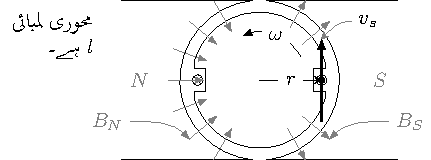
\includegraphics{figRotatingMachPrinciplesSingleTurnProducingEMF}
\begin{tikzpicture}
%grid
%\draw[gray] (-\sRo,-\sRo) grid (\sRo,\sRo);
%ROTOR
\pgfmathsetmacro{\shiftX}{5cm}
\pgfmathsetmacro{\pTheta}{150}
\pgfmathsetmacro{\pY}{0.2}
\rotor{2}{90}
%DOT on rotor
\draw (0:\rR-\pX) circle (2.5pt);
\draw[fill] (0:\rR-\pX) circle (1.5pt);
%CROSS on rotor
\draw (180:\rR-\pX) circle (2.5pt);
\draw (180:\rR-\pX)++(45:2.2pt)--++(-135:4.4pt);
\draw (180:\rR-\pX)++(-45:2.2pt)--++(135:4.4pt);
%STATOR
\draw ([shift={(-85:\sRi+\gap)}]0,0) arc (-85:85:\sRi+\gap);
\draw(85:\sRi+\gap)--++(0:1.2*\sRo);
\draw(-85:\sRi+\gap)--++(0:1.2*\sRo);
\node[very thick,gray] at (0:1.1*\sRo){$S$};
\draw ([shift={(95:\sRi+\gap)}]0,0) arc (95:270-5:\sRi+\gap);
\draw(95:\sRi+\gap)--++(180:1.2*\sRo);
\draw(-95:\sRi+\gap)--++(180:1.2*\sRo);
\node[very thick,gray] at (180:1.1*\sRo){$N$};
%flux at south pole
\foreach \angle in {-60,-40,40,60}{
\draw[gray,-latex] (0,0)++(\angle:\rR-2*\gap)--++(\angle:6*\gap);  }
%
\draw[gray,latex-] (0,0)++(-40:\rR+4*\gap) to [out=45,in=180] ++(1,0.3)node[right]{$B_S$};
%flux at north pole
\foreach \angle in {120,140,160,180,200,220,240}{
\draw[gray,latex-] (0,0)++(\angle:\rR-2*\gap)--++(\angle:6*\gap);  }
%
\draw[gray,latex-] (0,0)++(220:\rR+4*\gap) to [out=135,in=0] ++(-1,0.3)node[left]{$B_N$};
%velocity
\draw[thick,-latex](0:\rR-\pX)--++(0,-0.7)--++(0,1.4)coordinate (velocityTip);
\draw[gray,stealth-] (velocityTip) to [out=45,in=180] ++(0.5,0.3) node[right,text=black] {$v_s$};
%text
\draw[-stealth](0,0)--++(0:\rR-\pX) node[fill=white,pos=0.5]{$r$};
\draw[-latex]([shift={(30:0.7*\rR)}]0,0) arc (30:110:0.7*\rR);
\draw node[fill=white] at (70:0.7*\rR){$\omega$};
%
\draw node[align=right] at (-3.5,0.75){\RL{محوری لمبائی} \\ \RL{$l$ ہے۔}};
\end{tikzpicture}
\caption{ایک چکر کا لچھا مقناطیسی میدان میں گھوم رہا ہے۔}
\label{شکل_گھومتے_مشین_ایک_چکر_کی_پیدا_دباو}
\end{figure}

اس طرح حرکت کی مدد سے حاصل برقی دباو کو \اصطلاح{محرک برقی دباو}\فرہنگ{برقی دباو!محرک}\حاشیہب{electromotive force, emf}\فرہنگ{electromotive force}\فرہنگ{emf}  کہتے ہیں۔ روایتی طور پر کسی بھی طریقہ سے حاصل برقی دباو کو محرک برقی دباو کہتے ہیں۔ یوں کیمیائی برقی سیل وغیرہ کی برقی دباو بھی محرک برقی دباو کہلاتی  ہے۔

اس مساوات کو شکل \حوالہ{شکل_گھومتے_مشین_ایک_چکر_کی_پیدا_دباو} میں استعمال کرتے ہیں۔ گھومتے حصہ پر ایک چکر کا لچھا نسب ہے۔بائیں جانب خلاء میں لچھے کی برقی تار پر غور کریں۔مساوات \حوالہ{مساوات_گھومتے_مشین_قوت_لورینز}  کے تحت اس تار میں موجود مثبت برقی بار پر صفحہ کی عمودی سمت میں باہر کی جانب قوت اثر انداز ہو گی اور اس میں موجود منفی برقی بار پر اس کی اُلٹ سمت قوت عمل کرے گی۔اسی طرح مساوات \حوالہ{مساوات_گھومتے_مشین_برقی_دباو_تعریف}  کے تحت صفحہ سے باہر جانب برقی تار کا سرا برقی دباو  \عددیء{e} کا مثبت سرا ہو گا اور صفحہ کی اندر جانب برقی تار کا سرا برقی دباو \عددیء{e} کا منفی سرا ہو گا۔

اگر گھومتے حصہ کی محور پر نلکی محدد قائم کی جائے تو جنوبی مقناطیسی قطب کے سامنے خلاء میں \سمتیہ{B} رداس کی سمت میں ہے جبکہ شمالی مقناطیسی قطب کے سامنے  خلاء میں  \سمتیہ{B} رداس کی اُلٹ سمت میں ہے۔یوں جنوبی قطب کے سامنے شگاف میں برقی تار \سمتیہز{l}{S}  کے لئے ہم لکھ سکتے ہیں
\begin{gather}
\begin{aligned}
\kvec{v}_S&=v \atheta =\omega r \atheta\\
\kvec{B}_S&=B \ar\\
\kvec{l}_S&=l \az
\end{aligned}
\end{gather}
لہٰذا اس جانب لچھے کی ایک تار میں پیدا محرک برقی دباو
\begin{gather}
\begin{aligned}
e&=(\kvec{v} \times \kvec{B}) \cdot \kvec{l}\\
&=\omega r B l  (\atheta \times \ar) \cdot \az\\
&=\omega r B l  (-\az) \cdot \az\\
&=-\omega r B l 
\end{aligned}
\end{gather}
ہو گی۔

جنوبی مقناطیسی قطب کے سامنے شگاف میں برقی تار کی لمبائی کی سمت \عددیء{\az} لی گئی ہے۔اس مساوات میں برقی دباو کے منفی ہونے کا مطلب ہے کہ برقی تار کا مثبت سرا \عددیء{-\az} کی سمت میں ہے یعنی اس کا نچلا سرا مثبت اور اوپر والا سرا منفی ہے۔یوں اگر اس برقی تار میں برقی رو گزر سکے تو اس کی سمت \عددیء{-\az} یعنی صفحہ کی عمودی سمت میں اندر کی جانب ہو گی جسے شگاف میں دائرہ کے اندر صلیبی نشان سے ظاہر کیا گیا ہے۔ 

اسی طرح شمالی مقناطیسی قطب کے سامنے شگاف میں موجود برقی تار کے لئے ہم لکھ سکتے ہیں
\begin{gather}
\begin{aligned}
\kvec{v}_N&=v \atheta=\omega r \atheta\\
\kvec{B}_N&=-B \ar\\
\kvec{l}_N&=l \az
\end{aligned}
\end{gather}
اور یوں 
\begin{gather}
\begin{aligned}
e_N&=(\kvec{v}_N \times \kvec{B}_N)\cdot \kvec{l}_N\\
&=-\omega r B l (\atheta \times \ar) \cdot \az\\
&=-\omega r B l (-\az) \cdot \az\\
&=\omega r B l 
\end{aligned}
\end{gather}

شمالی مقناطیسی قطب کے سامنے شگاف میں برقی تار کی لمبائی کی سمت $\az$ لی گئی ہے۔اس مساوات میں برقی دباو کے مثبت ہونے کا مطلب ہے کہ برقی تار کا مثبت سرا $\az$ کی سمت میں ہے یعنی اس کا اوپر والا سرا مثبت اور نچلا  سرا منفی ہے۔یوں اگر اس برقی تار میں برقی رو گزر سکے تو اس کی سمت $\az$ یعنی صفحہ کی عمودی سمت میں باہر کی جانب ہو گی جسے شگاف میں دائرہ کے اندر نقطہ کے نشان سے دکھایا گیا ہے۔ 

یہ دو برقی تار مل کر ایک چکر کا لچھا بناتے ہیں۔ ان دونوں کے نچلے سرے سلسلہ وار جڑے ہیں جو شکل میں نہیں دکھایا گیا۔یوں اس لچھے کے اوپر نظر آنے والے سروں پر کُل برقی دباو \عددیء{e} ان دو برقی تاروں میں پیدا برقی دباو  کا مجموعہ ہو گا یعنی
\begin{gather}
\begin{aligned}
e&=2r l B \omega\\
&=A B \omega
\end{aligned}
\end{gather}
یہاں لچھے کا رقبہ  \عددیء{A=2 r l } ہے۔اگر ایک چکر سے اتنی برقی دباو حاصل ہوتی ہے تو \عددیء{N} چکر کے لچھے  سے
\begin{gather}
\begin{aligned}\label{مساوات_گھومتے_مشین_پیدا_دباو}
e&=\omega N A B\\
&=2 \pi f N A B\\
&=2 \pi f N \phi
\end{aligned}
\end{gather}
حاصل ہو گا۔

گھومتی آلوں میں خلائی درز میں  \سمتیہ{B} اور \سمتیہ{v}  ہر لمحہ عمودی ہوتے ہیں۔مساوات \حوالہ{مساوات_گھومتے_مشین_برقی_دباو_تعریف}  سے ظاہر ہے کہ اگر گھومنے کی رفتار اور محوری لمبائی معین ہوں تو پیدا کردہ برقی دباو  ہر لمحہ  \عددیء{B} کے براہِ راست متناسب ہو گا۔لہٰذا اگر خلائی درز میں زاویہ کے ساتھ  \عددیء{B} تبدیل ہو تو گھومتے لچھے میں پیدا برقی دباو بھی زاویہ کے ساتھ تبدیل ہو گا۔یوں جس شکل کی برقی دباو حاصل کرنی ہو اُسی شکل کی کثافتِ مقناطیسی دباو خلائی درز میں پیدا کرنی ہو گی۔اگر سائن نما برقی دباو پیدا کرنی مقصد ہو تو خلائی درز میں محیط پر سائن نما کثافتِ مقناطیسی بہاو ضروری ہے۔

اگلے حصے میں خلائی درز میں ضرورت کے تحت \عددیء{B}  پیدا کرنے کی ترکیب بتلائی جائے گی۔

\حصہ{پھیلے لچھے  اور سائن نما مقناطیسی دباو}
ہم نے اب تک جتنے مشین دیکھے ان سب میں گچھ\حاشیہب{non-distributed coils} لچھے دکھائے گئے۔ مزید یہ کہ ان آلوں میں گھومتے حصے پہ موجود مقناطیس کے \اصطلاح{اُبھرے قطب}\فرہنگ{قطب!ابھرے}\حاشیہب{salient poles}\فرہنگ{pole!salient} تھے۔ درحقیقت آلوں کے عموماً \اصطلاح{ہموار قطب}\فرہنگ{قطب!ہموار}\حاشیہب{non-salient poles}\فرہنگ{pole!non-salient} ہوتے ہیں اور ان میں \اصطلاح{پھیلے لچھے}\فرہنگ{لچھا!پھیلے}\حاشیہب{distributed winding}\فرہنگ{winding!distributed} پائے جاتے ہیں۔ ایسا کرنے سے ہم ساکن اور گھومتے حصوں کے درمیان خلائی درز میں سائن نما مقناطیسی دباو اور سائن نما  کثافتِ مقناطیسی بہاو پیدا کر سکتے ہیں۔ 
\begin{figure}
\centering
%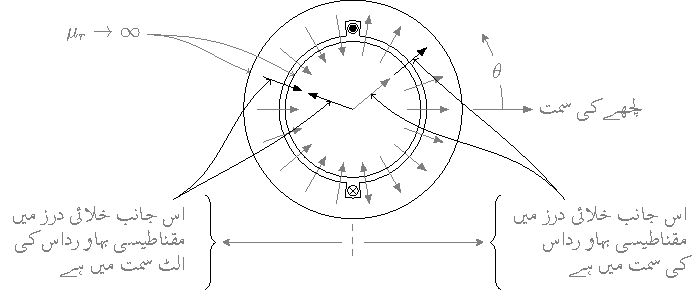
\includegraphics{figRotatingMachPrinciplesStatorCoilNotDistributed}
\begin{tikzpicture}
%
\stator{2}{90}
\slotDot{90}
\slotCross{270}
\draw (0,0) circle (\rR);
%FLUX
\foreach \angle in {-80,-60,-40,-20,0,20,40,60,80}{
\draw[gray,-latex] (\angle:0.8*\rR) --++(\angle:0.7); }
\foreach \angle in {100,120,140,160,180,200,220,240,260,280}{
\draw[gray,latex-] (\angle:0.8*\rR) --++(\angle:0.7); }
%text
\draw[gray,-latex] (0:1.1*\sRo)--++(0:1)node[right] {\RL{لچھے کا رخ}};
\draw[gray,-stealth]([shift={(0:1.1*\sRo+0.5)}]0,0) arc (0:30:1.1*\sRo+0.5);
\draw node[fill=white,text=gray] at (15:1.1*\sRo+0.5){$\theta$};
\draw[gray,dashed] (-90:\sRo+0.1)--++(0,-0.6);
%radial direction and flux
\draw[gray,-latex] (0,0) --(40:0.7*\rR)coordinate[pos=0.5](kradial);
\draw[-latex] (0,0) --(160:0.7*\rR)coordinate[pos=0.5](kradialO);
\draw[-latex] (40:0.8*\rR) --++(40:0.7)coordinate[pos=0.6](kflux); 
\draw[latex-] (160:0.8*\rR) --++(160:0.7)coordinate[pos=0.8](kfluxO); 
%text
\draw[gray,-stealth] (-90:\sRo+0.4)++(0.2,0) --++(2,0)node[xshift=0.4cm,right,align=right](kNOTopposing){\RL{اس جانب خلائی درز میں} \\ \RL{مقناطیسی بہاو رداسی} \\ \RL{رخ ہے}};
\draw[gray,-stealth] (-90:\sRo+0.4)++(-0.2,0) --++(-2,0)node[xshift=-0.5cm,left,align=right](kOpposing){\RL{اس جانب خلائی درز میں} \\ \RL{مقناطیسی بہاو رداسی} \\ \RL{رخ کے الٹ ہے}};
\draw[<-](kradial) to [out=-45,in=130] (kNOTopposing);
\draw[<-](kflux) to [out=-45,in=130] (kNOTopposing);
\draw[<-](kradialO) to [out=220,in=30] (kOpposing);
\draw[<-](kfluxO) to [out=220,in=30] (kOpposing);
\draw node[left,gray] at (160:2*\sRo)(kmu){$\mu_r \to \infty$};
\draw[<-,gray] (160:\sRo) to [out=160,in=0] (kmu);
\draw[<-,gray] (150:\rR) to [out=150,in=0] (kmu);
%brace
\draw[decorate,decoration={brace,amplitude=5pt}] (-90:\sRo+0.4)++(-0.5,0) ++(-2,0)++(0,0.8) -- ++(0,-1.6) node [black,midway,xshift=9pt] {};
\draw[decorate,decoration={brace,amplitude=5pt}] (-90:\sRo+0.4)++(0.5,0) ++(2,0)++(0,-0.8) -- ++(0,1.6) node [black,midway,xshift=9pt] {};
\end{tikzpicture}
\caption{ساکن لچھا گچھ کی شکل میں ہے۔}
\label{شکل_گھومتے_مشین_گچھ_لچھا}
\end{figure}

شکل \حوالہ{شکل_گھومتے_مشین_گچھ_لچھا}  میں ایک لچھا گچھ کی شکل کا دکھایا گیا ہے۔اس کے گھومنے والا حصہ گول شکل کا ہے اور اس کا \عددیء{\mu_r \to \infty} ہے۔ساکن حصے کا بھی \عددیء{\mu_r \to \infty} ہے۔ لچھے کا مقناطیسی دباو \عددیء{\tau=N i} ہے۔  یہ مقناطیسی دباو، مقناطیسی بہاو \عددیء{\phi}  کو جنم دیتا ہے جس کو ہلکی سیاہی کی  لکیروں سے ظاہر کیا گیا ہے۔ مقناطیسی بہاو کو لچھے کے گرد ایک چکر کاٹتے خلائی درز میں سے دو مرتبہ گزرنا پڑتا ہے۔ لہٰذا
\begin{align}
\tau=N i=2 H l_a
\end{align}
%
\begin{figure}
\centering
%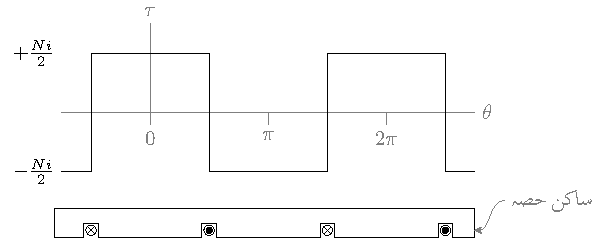
\includegraphics{figRotatingMachPrinciplesMMFjumpsAtDotAndCross}
\begin{tikzpicture}
%
\begin{scope}[yshift=-2cm]
\dotLinear{1,5}
\crossLinear{-1,3}
\slotSegment{-1/1,1/3,3/5}
\slotTop{-1/5}
\draw[gray,stealth-] (5.5,0) to [out=0,in=180] (6,0.5)node[right]{\RL{ساکن حصہ}};
\end{scope}
%
\draw[gray](-1.5,0)--(5.5,0)node[right]{$\theta$};
\draw[gray](0,0)--(0,1.5)node[above]{$\tau$};
\foreach \x/\labelText in {0/0,2/\pi,4/2\pi}{
\draw[gray](\x,0)--++(0,-0.2) node[below]{$\labelText$};}
\draw(-1.5,-1)--(-1,-1)--(-1,1)--(1,1)--(1,-1)--(3,-1)--(3,1)--(5,1)--(5,-1)--(5.5,-1);
%text
\draw node[left] at (-1.5,1){$+\tfrac{Ni}{2}$};
\draw node[left] at (-1.5,-1){$-\tfrac{Ni}{2}$};
\end{tikzpicture}
\caption{گچھ لچھے کی خلائی درز میں مقناطیسی دباو۔}
\label{شکل_گھومتے_مشین_گچھ_لچھے_کا_دباو}
\end{figure}

یوں ساکن لچھے کا آدھا مقناطیسی دباو ایک خلائی درز اور آدھا دوسرے خلائی درز میں مقناطیسی بہاو پیدا کرتا ہے۔ مزید یہ کہ خلائی درز میں کہیں پہ مقناطیسی دباو ( اور  مقناطیسی بہاو )،  رداس\حاشیہب{radius} کی سمت میں ہیں اور کہیں  پہ خلائی درز میں مقناطیسی دباو ( اور مقناطیسی بہاو )، رداس کی اُلٹی سمت میں ہیں۔ اگر ہم رداس کی سمت کو مثبت لیں تو   مقناطیسی بہاو ( اور مقناطیسی دباو ) \عددیء{-\tfrac{\pi}{2} < \theta< \tfrac{\pi}{2}} کے درمیان رداس ہی کی  سمت میں ہیں لہٰذا یہاں  یہ مثبت ہیں جبکہ باقی جگہ  مقناطیسی دباو ( اور مقناطیسی بہاو ) رداس کی اُلٹ سمت میں ہیں لہٰذا یہاں یہ منفی ہیں۔ ایسا ہی شکل \حوالہ{شکل_گھومتے_مشین_گچھ_لچھے_کا_دباو}  میں دکھایا گیا ہے۔ اس شکل میں خلائی درز میں مقناطیسی دباو کو زاویہ کے ساتھ ترسیم کیا گیا ہے۔\عددیء{-\tfrac{\pi}{2} < \theta <\tfrac{\pi}{2}} کے درمیان خلائی درز میں مقناطیسی دباو \عددیء{\tau_a} لچھے کے مقناطیسی دباو \عددیء{\tau} کا آدھا ہے اور اس کی سمت مثبت ہے جبکہ \عددیء{\tfrac{\pi}{2} < \theta <\tfrac{3 \pi}{2}} کی درمیان خلائی درز میں مقناطیسی دباو لچھے کے مقناطیسی دباو کے آدھا ہے اور اس کی سمت منفی ہے۔ یاد رہے کہ مقناطیسی دباو کی سمت\فرہنگ{مقناطیسی دباو!سمت} کا تعین رداس کی سمت سے کیا جاتا ہے۔

\جزوحصہ{بدلتی رو والے مشین}
بدلتی رو (اے سی) مشین بناتے وقت یہ کوشش کی جاتی ہے کہ خلائی درز میں مقناطیسی دباو سائن نما ہو۔ایسا کرنے کی خاطر لچھوں کو ایک سے زیادہ شگافوں میں تقسیم کیا جاتا ہے۔ اس سے سائن نما مقناطیسی دباو کیسے حاصل ہوتی ہے، اس بات کی  یہاں وضاحت کی جائے گی۔

\اصطلاح{فوریئر} تسلسل\فرہنگ{فوریئر تسلسل}\حاشیہب{Fourier series}\فرہنگ{Fourier series} کے تحت ہم کسی بھی تفاعل\حاشیہب{function} \عددیء{f(\theta_p)}  کو یوں لکھ سکتے ہیں۔
\begin{align}
f(\theta_p)=\sum_{n=0}^{\infty} (a_n \cos n \theta_p +b_n \sin n \theta_p)
\end{align}
اگر اس تفاعل کا دوری عرصہ\فرہنگ{دوری عرصہ}\حاشیہب{time period}\فرہنگ{time period} \عددیء{T} ہو تب
\begin{gather}
\begin{aligned}\label{مساوات_گھومتے_مشین_فورئر_تسلسل_جزو}
a_0&=\frac{1}{T} \int_{-T/2}^{T/2} f(\theta_p) \dif \theta_p\\
a_n&=\frac{2}{T} \int_{-T/2}^{T/2} f(\theta_p) \cos n \theta_p \dif \theta_p\\
b_n&=\frac{2}{T} \int_{-T/2}^{T/2} f(\theta_p) \sin n \theta_p \dif \theta_p
\end{aligned}
\end{gather}
کے برابر ہوں گے۔
%
\ابتدا{مثال}\شناخت{مثال_تبادلہ_توانائی_فوریئر_تسلسل}
شکل \حوالہ{شکل_گھومتے_مشین_گچھ_لچھے_کا_دباو}  میں دیئے گئے مقناطیسی دباو کا
\begin{itemize}
\item
فوریئر تسلسل حاصل کریں۔
\item
تیسری موسیقائی جز\فرہنگ{موسیقائی جزو}\حاشیہب{third harmonic component}\فرہنگ{harmonic} اور بنیادی جز\فرہنگ{بنیادی جزو}\حاشیہب{fundamental component}\فرہنگ{fundamental} کی نسبت معلوم کریں۔
\end{itemize}

حل:
\begin{itemize}
\item
مساوات \حوالہ{مساوات_گھومتے_مشین_فورئر_تسلسل_جزو}  کی مدد سے

\begin{align*}
a_0&=\frac{1}{2\pi} \left[\int_{-\pi}^{-\pi/2} \left(-\frac{Ni}{2} \right) \dif \theta_p+\int_{-\pi/2}^{\pi/2} \left (\frac{Ni}{2}\right) \dif \theta_p +\int_{\pi/2}^{\pi} \left(-\frac{Ni}{2}\right) \dif \theta_p  \right]\\
&=\frac{1}{2\pi} \left[\left(-\frac{Ni}{2} \right)\left(-\frac{\pi}{2}+\pi \right) +\left(\frac{Ni}{2} \right)\left(\frac{\pi}{2}+\frac{\pi}{2} \right)+\left(-\frac{Ni}{2} \right)\left(\pi-\frac{\pi}{2} \right)\right]\\
&=0
\end{align*}
اسی طرح
\begin{align*}
a_n&=\frac{2}{2\pi} \frac{Ni}{2} \left[\int_{-\pi}^{-\pi/2} -\cos n \theta_p \dif \theta_p +\int_{-\pi/2}^{\pi/2} \cos n \theta_p \dif \theta_p+\int_{\pi/2}^{\pi} -\cos n \theta_p \dif \theta_p\right]\\
&=\frac{Ni}{2\pi} \left[-\left. \frac{\sin n \theta_p}{n}\right|_{-\pi}^{-\pi/2} +\left. \frac{\sin n \theta_p}{n}\right|_{-\pi/2}^{\pi/2} -\left. \frac{\sin n \theta_p}{n}\right|_{\pi/2}^{\pi} \right]\\
&=\frac{Ni}{2n\pi} \left[\sin \frac{n\pi}{2}+2\sin \frac{n\pi}{2}+\sin \frac{n\pi}{2} \right]\\
&=\left(\frac{4}{n\pi}\right) \left( \frac{Ni}{2}\right) \sin \frac{n\pi}{2}
\end{align*}
اس مساوات میں \عددیء{n} کی قیمت ایک، دو، تین وغیرہ کے لئے ملتا ہے
\begin{align*}
a_1&=\left(\frac{4}{\pi}\right) \left( \frac{Ni}{2}\right), \quad a_3=-\left(\frac{4}{3\pi}\right) \left( \frac{Ni}{2}\right), \quad a_5=\left(\frac{4}{5\pi}\right) \left( \frac{Ni}{2}\right)\\
a_2&=a_4=a_6=0
\end{align*}
اسی طرح
\begin{align*}
b_n&=\frac{2}{2\pi} \frac{Ni}{2} \left[\int_{-\pi}^{-\pi/2} -\sin n \theta_p \dif \theta_p +\int_{-\pi/2}^{\pi/2} \sin n \theta_p \dif \theta_p+\int_{\pi/2}^{\pi} -\sin n \theta_p \dif \theta_p\right]\\
&=\frac{Ni}{2\pi} \left[\left. \frac{\cos n \theta_p}{n}\right|_{-\pi}^{-\pi/2} -\left. \frac{\cos n \theta_p}{n}\right|_{-\pi/2}^{\pi/2} +\left. \frac{\cos n \theta_p}{n}\right|_{\pi/2}^{\pi} \right]\\
&=0
\end{align*}
\item
ان جوابات سے
\begin{align*}
\abs{\frac{a_3}{a_1}} =\frac{\left(\frac{4}{3\pi}\right) \left( \frac{Ni}{2}\right)}{\left(\frac{4}{\pi}\right) \left( \frac{Ni}{2}\right)}=\frac{1}{3}
\end{align*}
\end{itemize}
حاصل ہوتا ہے۔لہٰذا تیسری موسیقائی جزو بنیادی جزو کے تیسرے حصے یعنی \عددیء{33.33} فی صد کے برابر ہے۔
\انتہا{مثال}
%
مثال \حوالہ{مثال_تبادلہ_توانائی_فوریئر_تسلسل} میں حاصل کئے گئے \عددیء{a_1,a_2,\cdots} استعمال کرتے ہوئے  ہم خلائی درز میں مقناطیسی دباو \عددیء{\tau} کا فوریئر تسلسل یوں لکھ سکتے ہیں۔
\begin{align}\label{مساوات_تبادلہ_توانائی_فوریئر_متقناطیسی_دباو_تسلسل}
\tau_a=\frac{4}{\pi}\frac{Ni}{2} \cos \theta_p-\frac{4}{3\pi}\frac{Ni}{2} \cos 3\theta_p+\frac{4}{5\pi}\frac{Ni}{2} \cos 5\theta_p+\cdots
\end{align}
مثال \حوالہ{مثال_تبادلہ_توانائی_فوریئر_تسلسل} سے ظاہر ہے کہ مقناطیسی دباو کے موسیقائی اجزاء  کی قیمتیں اتنی کم نہیں کہ انہیں رد کیا جا سکے۔جیسا آپ اس باب میں آگے دیکھیں گے کہ حقیقت میں استعمال ہونے والے  مقناطیسی دباو میں موسیقائی اجزاء قابلِ نظر انداز ہوں گے اور ہمیں صرف بنیادی جزو  سے غرض ہو گا۔اسی حقیقت کو مد نظر رکھتے ہوئے ہم  تسلسل کے موسیقائی اجزاء کو نظر انداز کرتے ہوئے اسی مساوات کو یوں لکھتے ہیں۔ 
\begin{align}
\tau_{a}=\frac{4}{\pi}\frac{Ni}{2} \cos \theta_p=\tau_0 \cos \theta_p
\end{align}
جہاں
\begin{align}\label{مساوات_گھومتے_مشین_دباو_چوٹی}
\tau_0=\frac{4}{\pi}\frac{Ni}{2} 
\end{align}
کے برابر ہے۔اس مساوات سے ہم دیکھتے ہیں کہ شکل \حوالہ{شکل_گھومتے_مشین_گچھ_لچھا}  میں لچھے سے حاصل مقناطیسی دباو بالکل اسی طرح ہے جیسے شکل \حوالہ{شکل_گھومتے_مشین_رداس_اور_مقناطیسی_بہاو}  میں سلاخ نما مقناطیس صفر زاویہ پر رکھے حالت میں دیتا۔ اگر یہاں یہ لچھا کسی ایسے زاویہ پر رکھا گیا ہوتا کہ اس سے حاصل مقناطیسی دباو زاویہ \عددیء{\theta_m}  پر زیادہ سے زیادہ ہوتا تو یہ بالکل شکل \حوالہ{شکل_گھومتے_مشین_رداس_اور_مقناطیسی_بہاو_مقناطیس_گھوما_ہے}  میں موجود مقناطیس کی طرح کا ہوتا۔ شکل \حوالہ{شکل_گھومتے_مشین_تین_دور_کے_لئے_لپٹی}  ایک ایسی ہی مثال ہے۔ ہم بالکل مساوات \حوالہ{مساوات_گھومتے_مشین_کثافت_بالمقابل_زاویہ}   کی طرح اس شکل میں لچھا  \عددیء{a} کے لئے لکھ سکتے ہیں۔
\begin{gather}
\begin{aligned}\label{مساوات_گھومتے_مشین_الف_موج}
\tau_a&=\tau_0 \cos \theta_{p_a}\\
\theta_{p_a}&=\theta-\theta_{m_a}=\theta-0\degree\\
\tau_a&=\tau_0 \cos (\theta-\theta_m)=\tau_0 \cos \theta
\end{aligned}
\end{gather}
اسی طرح لچھا \عددیء{b} اور \عددیء{c} کے  چونکہ \عددیء{\theta_{m_b}=120\degree} اور \عددیء{\theta_{m_c}=240\degree}  لہٰذا ان کے لئے ہم لکھ سکتے ہیں۔
\begin{gather}
\begin{aligned}\label{مساوات_گھومتے_مشین_ب_موج}
\tau_b&=\tau_0 \cos \theta_{p_b}\\
\theta_{p_b}&=\theta-\theta_{m_b}=\theta-120\degree\\
\tau_b&=\tau_0 \cos (\theta-\theta_{m_b})=\tau_0 \cos (\theta-120\degree)
\end{aligned}
\end{gather}
%
\begin{gather}
\begin{aligned}\label{مساوات_گھومتے_مشین_پ_موج}
\tau_c&=\tau_0 \cos \theta_{p_c}\\
\theta_{p_c}&=\theta-\theta_{m_c}=\theta-240\degree\\
\tau_c&=\tau_0 \cos (\theta-\theta_{m_c})=\tau_0 \cos (\theta-240\degree)
\end{aligned}
\end{gather}

اگرچہ ظاہری طور پر خلائی درز میں مقناطیسی دباو سائن نما ہرگز نہیں لگتا لیکن مساوات \حوالہ{مساوات_تبادلہ_توانائی_فوریئر_متقناطیسی_دباو_تسلسل}  ہمیں بتلاتی ہے کہ یہ محض آنکھوں کا دھوکہ ہے۔ اس مقناطیسی دباو کا بیشتر حصہ سائن نما ہی ہے۔  اب اگر ہم کسی طرح مساوات \حوالہ{مساوات_تبادلہ_توانائی_فوریئر_متقناطیسی_دباو_تسلسل}   میں پہلے رکن کے علاوہ باقی سب رکن کو صفر کر سکیں تو ہم بالکل  سائن نما مقناطیسی دباو حاصل کر سکتے ہیں۔
\begin{figure}
\centering
%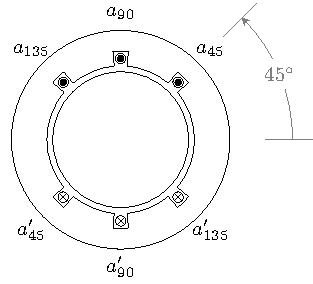
\includegraphics{figRotatingMachPrinciplesDistributedStatorWinding}
\begin{tikzpicture}
%grid
%\draw[gray] (-\sRo,-\sRo) grid (\sRo,\sRo);
%
\statorEach{45/90,90/135,135/225,225/270,270/315,315/405}
\draw (0,0) circle (\rR);
\slotDot{45,90,135}
\slotCross{-45,-90,-135}
\draw node at (45:\sRo+0.3) {$a_{45}$};
\draw node at (90:\sRo+0.3) {$a_{90}$};
\draw node at (135:\sRo+0.3) {$a_{135}$};
\draw node at (225:\sRo+0.3) {$a_{45}'$};
\draw node at (270:\sRo+0.3) {$a_{90}'$};
\draw node at (315:\sRo+0.3) {$a_{135}'$};
%text
\draw[gray] (0:\sRo+0.6)--++(0:0.7*\rR);
\draw[gray](45:\sRo+0.6)--++(45:0.7*\rR);
\draw[gray,-stealth] (0:\sRo+0.6+0.4*\rR) arc (0:45:\sRo+0.6+0.4*\rR);
\draw node[fill=white,text=gray] at (22.5:\sRo+0.6+0.4*\rR){$45\degree$};
\end{tikzpicture}%
\caption{پھیلا لچھا۔}
\label{شکل_گھومتے_مشین_پھیلا_لچھا}
\end{figure}

شکل \حوالہ{شکل_گھومتے_مشین_پھیلا_لچھا}  میں تقسیم شدہ لچھا دکھایا گیا ہے۔ یہاں شکل \حوالہ{شکل_گھومتے_مشین_گچھ_لچھا}  میں دکھائے گئے \عددیء{N} چکر کے لچھے کو تین چھوٹے یکساں لچھوں میں تقسیم کیا گیا ہے۔لہٰذا ان میں ہر چھوٹا لچھا \عددیء{\tfrac{N}{3}} چکر کا ہے۔  ایسے چھوٹے لچھوں کو سلسلہ وار جوڑا\فرہنگ{سلسلہ وار}\حاشیہب{series connected} جاتا ہے اور  یوں ان میں یکساں  برقی رو \عددیء{i} گزرے گی۔ ان تین لچھوں کو تین مختلف شگافوں میں رکھا گیا ہے۔پہلے لچھے کو شگاف \عددیء{a_{45}} اور \عددیء{a_{45}'} میں رکھا گیا ہے۔ دوسرے لچھے کو شگاف \عددیء{a_{90}} اور \عددیء{a_{90}'} میں اور تیسرے لچھے کو شگاف \عددیء{a_{135}} اور \عددیء{a_{135}'} میں رکھا گیا ہے۔
\begin{figure}
\centering
%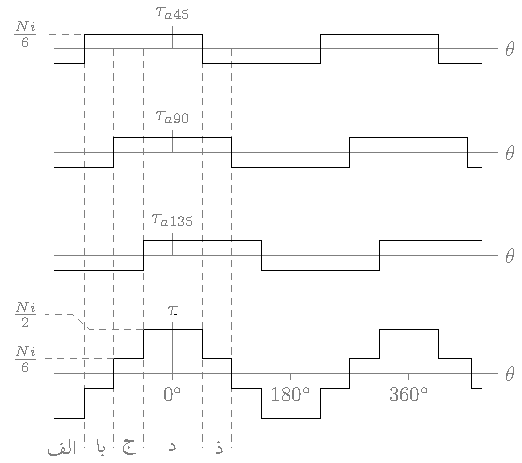
\includegraphics{figRotatingMachPrinciplesMMFjumpsThreePhase}
\begin{tikzpicture}
%
\pgfmathsetmacro{\j}{0.25}
\pgfmathsetmacro{\shiftY}{0.5}
%
%dashed vertical lines
\draw[gray,dashed](-135/90,0)--++(0,-11*\shiftY-5*\j)node[left]{\textup{الف}};
\draw[gray,dashed](-90/90,0)--++(0,-11*\shiftY-5*\j)node[left]{\textup{با}};
\draw[gray,dashed](-45/90,0)--++(0,-11*\shiftY-5*\j)node[left]{\textup{ج}};
\draw[gray,dashed](45/90,0)--++(0,-11*\shiftY-5*\j)node[xshift=-0.5 cm]{\textup{د}};
\draw[gray,dashed](90/90,0)--++(0,-11*\shiftY-5*\j)node[left]{\textup{ذ}};
%axis
\draw[gray](-2,0)--(5.5,0)node[right]{$\theta$};
\draw[gray](0,0)--(0,1.5*\j)node[above]{$\tau_{a45}$};
%\draw (-45/90,0)--++(0,-0.2)node[below,gray]{$-45\degree$};
%
\mmf{-180/-\j/-135/\j,-135/\j/45/-\j,45/-\j/225/\j,225/\j/405/-\j}
\draw(405/90,-\j)--(470/90,-\j);
%text
\draw[gray,dashed]  (-140/90,\j)--++(-0.6,0)node[left,solid]{$\tfrac{N i}{6}$};
%
\begin{scope}[yshift=-3.5*\shiftY cm]
%axis
\draw[gray](-2,0)--(5.5,0)node[right]{$\theta$};
\draw[gray](0,0)--(0,1.5*\j)node[above]{$\tau_{a90}$};;
%
\mmf{-180/-\j/-90/\j,-90/\j/90/-\j,90/-\j/270/\j,270/\j/450/-\j}
\draw(450/90,-\j)--(470/90,-\j);
\end{scope}
%
\begin{scope}[yshift=-7*\shiftY cm]
%axis
\draw[gray](-2,0)--(5.5,0)node[right]{$\theta$};
\draw[gray](0,0)--(0,1.5*\j)node[above]{$\tau_{a135}$};
%\draw(45/90,0)--++(0,-0.2)node[below,gray]{$45\degree$};
%
\mmf{-180/-\j/-45/\j,-45/\j/135/-\j,135/-\j/315/\j}
\draw(315/90,\j)--(470/90,\j);
\end{scope}
%
\begin{scope}[yshift=-11*\shiftY cm,xscale=1/90]   %,xscale=1/3 cm
%axis
\draw[gray](-2*90,0)--(5.5*90,0)node[right]{$\theta$};
\draw[gray](0,0)--(0,3.5*\j)node[above]{$\tau$};
\draw[gray] (0,0)--++(0,-0.1)node[below]{$0\degree$};
\draw[gray] (180,0)--++(0,-0.1)node[below]{$180\degree$};
\draw[gray] (360,0)--++(0,-0.1)node[below]{$360\degree$};
%
\draw(-180,-3*\j)--(-135,-3*\j)--(-135,-\j)--(-90,-\j)--(-90,\j)--(-45,\j)--(-45,3*\j)--(45,3*\j)--(45,\j)--(90,\j)--(90,-\j)--(135,-\j)--(135,-3*\j)--(225,-3*\j)--(225,-\j)--(270,-\j)--(270,\j)--(315,\j)--(316,3*\j)--(405,3*\j)--(405,\j)--(455,\j)--(455,-\j)--(470,-\j);
\draw(315/90,1)--(470/90,1);
%text
\draw[gray,dashed]  (-90,\j)--(-140-0.6*90,\j)node[left,solid]{$\tfrac{N i}{6}$};
\draw[gray,dashed]  (-45,3*\j)--++(-0.9*90,0)--++(-0.3*90,\j)--(-140-0.6*90,4*\j)node[left,solid]{$\tfrac{N i}{2}$};
\end{scope}
\end{tikzpicture}
\caption{پھیلے لچھے کا کُل مقناطیسی دباو۔}
\label{شکل_گھومتے_مشین_پھیلے_لچھے_کی_دباو}
\end{figure}


شگافوں کے ایک جوڑے کو ایک ہی طرح کے نام دیئے گئے ہیں، البتہ ایک شگاف کو \عددیء{a} اور دوسرے کو \عددیء{a'} نام دیا گیا ہے۔یوں شگافوں کا پہلے جوڑا  \عددیء{a_{45}} اور \عددیء{a_{45}'}  ہے۔ \عددیء{a}  شگافوں کے نام ان کے زاویوں کی نسبت سے رکھے گئے ہیں۔لہٰذا شگاف  \عددیء{a_{45}} درحقیقت \عددیء{45\degree} زاویہ پر ہے، شگاف \عددیء{a_{90}} نوے درجہ زاویہ پر اور شگاف \عددیء{a_{135}}  ایک سو پینتیس درجہ زاویہ پر ہے۔

چونکہ ہر لچھا \عددیء{\tfrac{N}{3}} چکر کا ہے اور ان سب میں یکساں برقی رو \عددیء{i} ہے،  لہٰذا  شکل \حوالہ{شکل_گھومتے_مشین_پھیلا_لچھا}   میں دیئے گئے پھیلے لچھے سے حاصل مقناطیسی دباو کا زاویہ کے ساتھ ترسیم شکل \حوالہ{شکل_گھومتے_مشین_پھیلے_لچھے_کی_دباو}  کے نچلے ترسیم کی طرح ہو گا۔اس شکل میں سب سے اُوپر لچھا  \عددیء{a_{45}}  کے مقناطیسی دباو کا ترسیم ہے۔ یہ بالکل شکل \حوالہ{شکل_گھومتے_مشین_گچھ_لچھے_کا_دباو}  میں دیئے ترسیم کی طرح ہے البتہ یہ صفر زاویہ سے \عددیء{-45\degree} ہٹ کر ہے۔اُوپر سے دوسرا ترسیم لچھا \عددیء{a_{90}} کا ہے جو ہو بہو شکل  کی طرح ہے جبکہ اس سے نیچے لچھا \عددیء{a_{135}} کا ترسیم ہے جو صفر زاویہ سے \عددیء{+45\degree} ہٹ کر ہے۔ان تینوں ترسیمات میں طول \عددیء{\tfrac{Ni}{6}} ہے۔

ان تینوں ترسیمات سے کُل مقناطیسی دباو کا ترسیم یوں حاصل ہوتا ہے۔اس شکل میں عمودی نقطہ دار لکیریں لگائی گئی ہیں۔ بائیں جانب پہلی لکیر کی بائیں طرف علاقے کو الف کہا گیا ہے۔اس علاقے میں پہلے تینوں ترسیمات کی مقدار \عددیء{-\tfrac{Ni}{6}} ہے لہٰذا ان کا مجموعہ \عددیء{-\tfrac{Ni}{2}} ہو گا۔یہی سب سے نچلے کُل مقناطیسی دباو کی ترسیم میں دکھایا گیا ہے۔ اسی طرح علاقہ ب میں پہلے ترسیم کی مقدار \عددیء{+\tfrac{Ni}{6}} ، دوسری ترسیم کی \عددیء{-\tfrac{Ni}{6}} اور تیسری کی بھی \عددیء{-\tfrac{Ni}{6}} ہے۔ ان کا مجموعہ \عددیء{-\tfrac{Ni}{6}} بنتا ہے جو کُل مقناطیسی دباو ہے۔علاقہ ج میں
 \عددیء{+\tfrac{Ni}{6}}، \عددیء{+\tfrac{Ni}{6}} اور \عددیء{-\tfrac{Ni}{6}} غیر سمتیں ہیں جن کا مجموعہ \عددیء{+\tfrac{Ni}{6}} ہی کُل مقناطیسی دباو ہے جو سب سے نچلے ترسیم میں دکھایا گیا ہے۔ اسی طرح آپ پورا ترسیم کھینچ سکتے ہیں۔

شکل \حوالہ{شکل_گھومتے_مشین_پھیلے_لچھے_کی_دباو}  کے نچلے ترسیم کو شکل \حوالہ{شکل_گھومتے_مشین_پھیلے_لچھے_نقطہ_صلیب_پر_جمپ}  میں دوبارہ دکھایا گیا ہے۔
\begin{figure}
\centering
%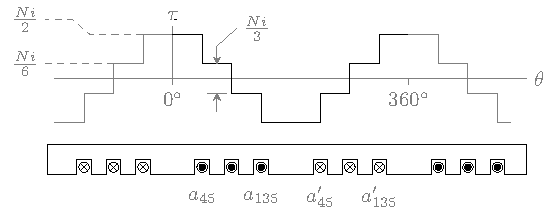
\includegraphics{figRotatingMachPrinciplesDistributedWindingDotAndCross}
\begin{tikzpicture}
%
\pgfmathsetmacro{\j}{0.25}
\pgfmathsetmacro{\shiftY}{-1.5 cm}
%

\begin{scope}[xscale=1/90]   %,xscale=1/3 cm
%axis
\draw[gray](-2*90,0)--(6*90,0)node[right]{$\theta$};
\draw[gray](0,0)--(0,3.5*\j)node[above]{$\tau$};
%
\draw[gray](-180,-3*\j)--(-135,-3*\j)--(-135,-\j)--(-90,-\j)--(-90,\j)--(-45,\j)--(-45,3*\j)--(0,3*\j);
\draw (0,3*\j)--(45,3*\j)--(45,\j)--(90,\j)--(90,-\j)--(135,-\j)--(135,-3*\j)--(225,-3*\j)--(225,-\j)--(270,-\j)--(270,\j)--(315,\j)--(315,3*\j)--(360,3*\j);
\draw[gray] (360,3*\j)--(405,3*\j)--(405,\j)--(450,\j)--(450,-\j)--(495,-\j)--(495,-3*\j)--(515,-3*\j);
\draw(315/90,1)--(470/90,1);
%text
\draw[gray] (0,0)--(0,-0.1)node[gray,below]{$0\degree$};
\draw[gray] (360,0)--(360,-0.1)node[gray,below]{$360\degree$};
\draw[gray,dashed]  (-90,\j)--(-140-0.6*90,\j)node[left,solid]{$\tfrac{N i}{6}$};
\draw[gray,dashed]  (-45,3*\j)--++(-0.9*90,0)--++(-0.3*90,\j)--(-140-0.6*90,4*\j)node[left,solid]{$\tfrac{N i}{2}$};
%
\draw[gray,stealth-] (67.5,\j)--++(0,0.3)--++(30,0.3)node[right]{$\tfrac{N i}{3}$};
\draw[gray,stealth-](67.5,-\j)--++(0,-0.3);
\draw[gray](67.5,-\j)++(-15,0)--++(30,0);
\end{scope}
%
\begin{scope}[yshift=\shiftY]
\dotLinear{0.5,1,1.5,4.5,5,5.5}
\crossLinear{-1.5,-1,-0.5,2.5,3,3.5}
\slotSegment{-1.5/-1,-1/-0.5,-0.5/0.5,0.5/1,1/1.5,1.5/2.5,2.5/3,3/3.5,3.5/4.5,4.5/5,5/5.5}
\slotTop{-1.5/5.5}
%text
\draw node[gray] at (0.5,-0.5) {$a_{45}$};
\draw node[gray] at (1.5,-0.5) {$a_{135}$};
\draw node[gray] at (2.5,-0.5) {$a_{45}'$};
\draw node[gray] at (3.5,-0.5) {$a_{135}'$};
\end{scope}
\end{tikzpicture}
\caption{پھیلے لچھے کا مقناطیسی دباو۔}
\label{شکل_گھومتے_مشین_پھیلے_لچھے_نقطہ_صلیب_پر_جمپ}
\end{figure}

شکل \حوالہ{شکل_گھومتے_مشین_پھیلے_لچھے_نقطہ_صلیب_پر_جمپ}  کا اگر شکل \حوالہ{شکل_گھومتے_مشین_پھیلے_لچھے_کی_دباو}  کے ساتھ تقابل کیا جائے تو محض دیکھنے سے بھی یہ
 ظاہر ہے کہ شکل \حوالہ{شکل_گھومتے_مشین_پھیلے_لچھے_نقطہ_صلیب_پر_جمپ}   زیادہ سائن نما موج کے نوعیت کا ہے۔ ہمیں فوریئر تسلسل حل کرنے سے بھی یہی نتیجہ ملتا ہے۔ہم دیکھ سکتے ہیں کہ  شگافوں کی جگہ اور ان میں لچھوں کے چکر کو یوں رکھا جا سکتا ہے کہ ان سے پیدا کردہ مقناطیسی دباو سائن نما کے زیادہ سے زیادہ قریب ہو۔

چونکہ پھیلے لچھے کے مختلف حصے ایک ہی زاویہ پہ مقناطیسی دباو نہیں بناتے لہٰذا ان سے حاصل کُل مقناطیسی دباو کا حیطہ ایک گچھ لچھے  کے حیطہ سے قدرِ کم ہوتا ہے۔اس اثر کو مساوات \حوالہ{مساوات_گھومتے_مشین_دباو_چوٹی} میں جزو \عددیء{k_w} کے ذریعہ یوں ظاہر کیا جاتا ہے۔
\begin{gather}
\begin{aligned}
\tau_0&=k_w \frac{4}{\pi}\frac{N i}{2}\\
\tau_{a}&=k_w \frac{4}{\pi}\frac{N i}{2} \cos \theta=\tau_0 \cos \theta \label{مساوات_گھومتے_مشین_دباو_سائن_نما}
\end{aligned}
\end{gather}
اس مساوات میں \عددیء{k_w} کو \اصطلاح{جزو  پھیلاو}\فرہنگ{جزو!پھیلاو}\حاشیہب{winding factor}\فرہنگ{winding factor}  کہتے ہیں۔ یہ  اکائی سے قدرِ کم ہوتا ہے یعنی
\begin{align}
0<k_w<1
\end{align}
%
\ابتدا{مثال}
شکل \حوالہ{شکل_گھومتے_مشین_پھیلا_لچھا}  میں دیئے گئے پھیلے لچھے کے لئے \عددیء{k_w} معلوم کریں۔
\begin{figure}
\centering
%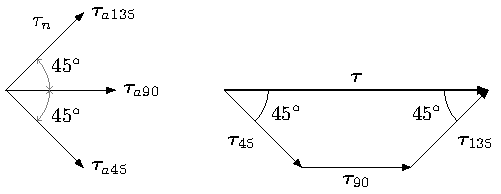
\includegraphics{figRotatingMachPrinciplesDistributedWindingFactor}
\begin{tikzpicture}
%
\draw[-latex](0,0)--(0:\sRo)node[right]{${\bm{\tau}}_{a90}$};
\draw[-latex](0,0)--(45:\sRo)node[right]{${\bm{\tau}}_{a135}$}node[pos=0.7,above left]{$\tau_n$};
\draw[-latex](0,0)--(-45:\sRo)node[right]{${\bm{\tau}}_{a45}$};
\draw[gray,<->] (0:0.4*\sRo) arc (0:45:0.4*\sRo);
\draw node at (22.5:0.6*\sRo){$45\degree$};
\draw[gray,<->] (0:0.4*\sRo) arc (0:-45:0.4*\sRo);
\draw node at (-22.5:0.6*\sRo){$45\degree$};
%
\begin{scope}[xshift=2*\sRo cm]
\draw[-latex](0,0)--(-45:\sRo)node[below left,pos=0.5]{${\bm{\tau}}_{45}$};
\draw[-latex](-45:\sRo)--++(0:\sRo)node[below,pos=0.5]{${\bm{\tau}}_{90}$};
\draw[-latex] (-45:\sRo)++(0:\sRo)--++(45:\sRo)node[below right,pos=0.5]{${\bm{\tau}}_{135}$} coordinate(netFlux);
\draw[thick,-latex](0,0)--(netFlux)node[above,pos=0.5]{${\bm{\tau}}$};
\draw(0:0.4*\sRo) arc (0:-45:0.4*\sRo);
\draw node at (-20:0.6*\sRo){$45\degree$};
\draw(netFlux)--++(180:0.4*\sRo) arc (180:225:0.4*\sRo);
\draw (netFlux)++(200:0.6*\sRo)node{$45\degree$};
\end{scope}
\end{tikzpicture}
\caption{پھیلے لچھے کا جزو پھیلاو۔}
\label{شکل_گھومتے_مشین_جزو_پھیلاو}
\end{figure}

حل: شکل  \حوالہ{شکل_گھومتے_مشین_جزو_پھیلاو} سے رجوع کریں۔ یہ تین چھوٹے لچھے برابر مقناطیسی دباو \عددیء{\tau_n=\tfrac{4}{\pi}\tfrac{ni}{2}} پیدا کرتے ہیں، البتہ ان کی سمتیں مختلف ہیں۔یہاں چونکہ ایک لچھا  \عددیء{\tfrac{N}{3}} چکر کا ہے لہٰذا \عددیء{n=\tfrac{N}{3}} ہے۔ ہم ان سمتیوں کو جمع کر کے ان کا مجموعی مقناطیسی دباو \عددیء{\tau} معلوم کرتے ہیں۔
\begin{align*}
\tau_a&=\tau_n \cos 45\degree+\tau_n+\tau_n \cos 45\degree\\
&=2.4142 \tau_n
\end{align*}
یعنی
\begin{align*}
\tau_a=2.4142 \frac{4}{\pi}\frac{ni}{2}=\frac{2.4142}{3} \frac{4}{\pi}\frac{N i}{2}=0.8047 \frac{4}{\pi}\frac{N i}{2}
\end{align*}
لہٰذا \عددیء{k_w=0.8047} کے برابر ہے۔
\انتہا{مثال}
%
\ابتدا{مثال}
ایک تین دور \عددیء{50} ہرٹز پر چلنے والا ستارہ نما جڑے جنریٹر کو  \عددیء{3000} چکر فی منٹ کی رفتار سے چلایا جا رہا ہے۔تیس چکر کے میدانی لچھے  کا جزو پھیلاو \عددیء{k_{w,m}=0.9} جبکہ پندرہ چکر قوی لچھے کا جزو پھیلاو \عددیء{k_{w,q}=0.833} ہیں۔مشین کا رداس \عددیء{0.7495} میٹر اور اس  کی لمبائی \عددیء{l=2.828} میٹر ہیں۔خلائی درز \عددیء{l_k=0.04} میٹر ہے۔اگر اس کے میدانی لچھے میں \عددیء{1000}  ایمپیئر برقی رو ہے تو معلوم کریں
\begin{itemize}
\item
میدانی مقناطیسی دباو کی زیادہ سے زیادہ مقدار۔
\item
خلائی درز میں کثافتِ مقناطیسی بہاو۔
\item
ایک قطب پر مقناطیسی بہاو۔
\item
محرک تار پر برقی دباو۔
\end{itemize}

حل:
\begin{itemize}
\item
\begin{align*}
\tau_0&=k_{w,m} \frac{4}{\pi}\frac{N_m i_m}{2}=0.9 \times \frac{4}{\pi} \times \frac{30 \times 1000}{2}=\SI{17186}{\ampere \cdot turns \per \meter}
\end{align*}
\item
\begin{align*}
B_0&=\mu_0 H_0=\mu_0 \frac{\tau_0}{l_k}=4 \pi 10^{-7} \times \frac{17186}{0.04}=\SI{0.54}{\tesla}
\end{align*}
\item
\begin{align*}
\phi_0&=2 B_0 l r =2 \times 0.54 \times 2.828 \times 0.7495=\SI{2.28915}{\weber}
\end{align*}
\item
\begin{align*}
E_{rms}&=4.44 f k_{w,q} N_q \phi_0\\
&=4.44 \times 50 \times 0.833 \times 15 \times 2.28915\\
&=\SI{6349.85}{\volt} 
\end{align*}
\end{itemize}
لہٰذا ستارہ جڑی جنریٹر کی تار کی برقی دباو
\begin{align*}
\sqrt{3} \times 6349.85 \approx \SI{11000}{\volt}
\end{align*}
ہو گی۔
\انتہا{مثال}
%
جیسا پہلے ذکر ہوا ہم چاہتے ہیں کہ سائن نما مقناطیسی دباو حاصل کر سکیں۔ چھوٹے لچھوں کے چکر اور شگافوں کی جگہ یوں چنے جاتے ہیں کہ یہ بنیادی مقصد پورا ہو۔ شکل \حوالہ{شکل_گھومتے_مشین_پھیلے_لچھے_نقطہ_صلیب_پر_جمپ}  میں ہم دیکھتے ہیں کہ صفر زاویہ کی دونوں جانب مقناطیسی دباو کی موج یکساں طور پر گھٹتی یا بڑھتی ہے۔ یعنی جمع اور منفی  پینتالیس زاویہ پر مقناطیسی دباو  \عددیء{\tfrac{Ni}{3}}  گھٹ جاتی ہے۔ اسی طرح جمع اور منفی نوے زاویہ پر یہ یکساں طور پر مزید گھٹتی ہے، وغیرہ وغیرہ۔ یہ ایک بنیادی اصول ہے جس کا خیال رکھنا ضروری ہے۔

چھوٹے لچھوں کے چکر اور شگافوں کی جگہوں کا فیصلہ فوریئر تسلسل کی مدد سے کیا جاتا ہے۔فوریئر تسلسل میں موسیقائی جزو کم سے کم اور اس میں بنیادی جزو زیادہ سے زیادہ رکھے جاتے ہیں۔

ساکن لچھوں کی طرح حرکت کرتے لچھوں کو بھی ایک سے زیادہ چھوٹے لچھوں میں تقسیم کیا جاتا ہے تا کہ سائن نما مقناطیسی دباو حاصل ہو۔

\حصہ{مقناطیسی دباو کی گھومتی موجیں}
گھومتے آلوں میں لچھوں کو برقی دباو دیا جاتا ہے جس سے اس کا گھومنے والا حصہ حرکت میں آتا ہے۔ یہاں ہم اس بات کا مطالعہ کرتے ہیں کہ یہ گھومنے کی حرکت کیسے پیدا ہوتی ہے۔

\جزوحصہ{ایک دور کی لپٹی مشین}
مساوات \حوالہ{مساوات_گھومتے_مشین_دباو_سائن_نما}  میں ایک لچھے کی مقناطیسی دباو یوں دی گئی ہے۔
\begin{align}
\tau_a=k_w \frac{4}{\pi}\frac{Ni}{2} \cos \theta
\end{align}
 اگر اس لچھے میں مقناطیسی بہاو بھی سائن نما ہو یعنی
\begin{align}
i_a=I_0 \cos \omega t
\end{align}
تو 
\begin{align}\label{مساوات_گھومتے_مشین_دباو_زاویہ_اور_وقت_پر_منحصر}
\tau_a=k_w \frac{4}{\pi} \frac{N I_0}{2} \cos \theta \cos \omega t=\tau_0 \cos \theta \cos \omega t
\end{align}
ہو گا جہاں
\begin{align}
\tau_0=k_w \frac{4}{\pi} \frac{N I_0}{2}
\end{align}
کے برابر ہے۔مساوات \حوالہ{مساوات_گھومتے_مشین_دباو_زاویہ_اور_وقت_پر_منحصر}  کہتا ہے کہ یہ مقناطیسی دباو زاویہ \عددیء{\theta} اور لمحہ \عددیء{t} کے ساتھ تبدیل ہوتا ہے۔ اس مساوات کو ہم مندرجہ ذیل قلیہ سے دو ٹکڑوں میں توڑ سکتے ہیں۔
\begin{align*}
\cos \alpha \cos \beta =\frac{\cos (\alpha +\beta) +\cos (\alpha -\beta)}{2}
\end{align*}
لہٰذا
\begin{align}
\tau_a=\tau_0 \left [\frac{\cos (\theta +\omega t) +\cos (\theta -\omega t)}{2}\right]=\tau_a^{-}+\tau_a^{+}
\end{align}
لکھا جا سکتا ہے۔یوں
\begin{align}
\tau_a^{-}&=\frac{\tau_0}{2} \cos (\theta +\omega t)\\
\tau_a^{+}&=\frac{\tau_0}{2} \cos (\theta -\omega t)
\end{align}
ہیں۔اس مساوات سے یہ بات سامنے آتی ہے کہ درحقیقت یہ مقناطیسی دباو دو اُلٹ سمتوں میں گھومنے والے مقناطیسی دباو کی موجیں ہیں۔ اس کا پہلا جزو \عددیء{\tau_a^-} زاویہ \عددیء{\theta} گھٹنے کی جانب گھومتا ہے یعنی گھڑی کی سمت میں اور اس کا دوسرا جزو \عددیء{\tau_a^+} گھڑی کی اُلٹی سمت گھومتا ہے یعنی یہ زاویہ بڑھنے کی جانب گھومتا ہے۔

ایک دور کی لپٹی آلوں میں یہ کوشش کی جاتی ہے کہ ان دو گھومتے مقناطیسی دباو میں سے ایک کو بالکل ختم یا کم سے کم کیا جائے۔ اس طرح کرنے سے ایک ہے سمت میں کُل مقناطیسی دباو گھومتا ملتا ہے جو بالکل اسی طرح کا ہوتا ہے جیسے ایک مقناطیس گھمایا جا رہا ہو۔ تین دور کے آلوں میں یہ کرنا نہایت آسان ہوتا ہے لہٰذا انہیں پہلے سمجھ لینا زیادہ بہتر ہو گا۔

\جزوحصہ{تین دور کی لپٹی مشین کا تحلیلی تجزیہ}
شکل \حوالہ{شکل_گھومتے_مشین_تین_دور_کے_لئے_لپٹی}  میں تین دور کی لپٹی مشین دکھائی گئی ہے۔مساوات \حوالہ{مساوات_گھومتے_مشین_الف_موج} ، \حوالہ{مساوات_گھومتے_مشین_ب_موج}  اور \حوالہ{مساوات_گھومتے_مشین_پ_موج}  میں ایسے تین لچھوں کی فوریئر تسلسل کی بنیادی جزو دیئے گئے ہیں جو کے یہ ہیں۔
\begin{gather}
\begin{aligned}\label{مساوات_گھومتے_مشین_تین_دباو_الف}
\tau_a&=k_w \frac{4}{\pi}\frac{N_a i_a}{2}\cos \theta\\
\tau_b&=k_w \frac{4}{\pi}\frac{N_b i_b}{2}\cos (\theta-120\degree)\\
\tau_c&=k_w \frac{4}{\pi}\frac{N_c i_c}{2}\cos (\theta+120\degree)
\end{aligned}
\end{gather}
%
\begin{figure}
\centering
%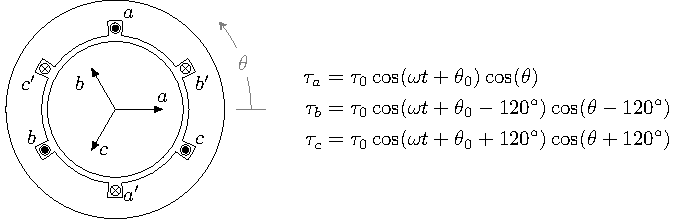
\includegraphics{figRotatingMachPrinciplesThreePhaseSynchronousMachine}
\begin{tikzpicture}
%grid
%\draw[gray] (-\sRo,-\sRo) grid (\sRo,\sRo);
\pgfmathsetmacro{\shiftX}{5cm}
\stator{6}{30}
\slotDot{90,210,330}
\slotCross{30,150,270}
%\slotName{comma separated angles/name/NameAtleftORrightOfSlot}
\slotName{90/a/above right,210/b/above left,330/c/above right}
\slotName{30/b'/below right,150/c'/below left,270/a'/right}
%
\draw (0,0) circle (\rR);
\draw[-latex] (0,0)--++(0:0.7*\rR)node [above]{$a$};
\draw[-latex] (0,0)--++(120:0.7*\rR)node [below left]{$b$};
\draw[-latex] (0,0)--++(-120:0.7*\rR)node [right]{$c$};
%
\draw[gray](0:\sRo+0.2)--++(0:0.5 )coordinate[pos=0.5] (angleZero);
\draw[gray,-stealth](angleZero) arc (0:40:\sRo+0.2+0.25);
\draw node[gray,fill=white] at (20:\sRo+0.2+0.25){$\theta$};
%
\begin{scope}[xshift=3 cm ]
\draw node[right] at (0,0){$\begin{aligned}
\tau_a&=\tau_0 \cos (\omega t+\theta_0) \cos (\theta)\\
\tau_b&=\tau_0 \cos (\omega t+\theta_0-120\degree) \cos (\theta-120\degree)\\
\tau_c&=\tau_0 \cos (\omega t+\theta_0+120\degree) \cos (\theta+120\degree)
\end{aligned}
$};
\end{scope}
\end{tikzpicture}
\caption{تین دور کی لپٹی مشین۔}
\label{شکل_گھومتے_مشین_تین_دور_کے_لئے_لپٹی}
\end{figure}
اگر ان تین لچھوں میں تین دوری برقی رو ہو یعنی
\begin{gather}
\begin{aligned}\label{مساوات_گھومتے_مشین_تین_برقی_رو}
i_a&=I_0 \cos (\omega t+\alpha)\\
i_b&=I_0 \cos (\omega t +\alpha -120\degree)\\
i_c&=I_0 \cos (\omega t +\alpha +120\degree)
\end{aligned}
\end{gather}
تو بالکل مساوات \حوالہ{مساوات_گھومتے_مشین_دباو_زاویہ_اور_وقت_پر_منحصر} کی طرح ہم مساوات \حوالہ{مساوات_گھومتے_مشین_تین_برقی_رو}  کی مدد سے مساوات \حوالہ{مساوات_گھومتے_مشین_تین_دباو_الف} کو یوں لکھ سکتے ہیں۔
\begin{gather}
\begin{aligned}
\tau_a&=k_w \frac{4}{\pi}\frac{N_a I_0}{2} \cos \theta \cos (\omega t +\alpha)\\
\tau_b&=k_w \frac{4}{\pi}\frac{N_b I_0}{2} \cos (\theta -120\degree)\cos (\omega t +\alpha -120\degree)\\
\tau_c&=k_w \frac{4}{\pi}\frac{N_c I_0}{2} \cos (\theta +120\degree)\cos (\omega t +\alpha +120\degree)
\end{aligned}
\end{gather}
اگر
\begin{align*}
N_a=N_b=N_c=N
\end{align*}
ہو تو انہیں
\begin{gather}
\begin{aligned}\label{مساوات_تبادلہ_تین_گھومتے_دباو}
\tau_a&=\frac{\tau_0}{2} \left[\cos (\theta +\omega t +\alpha) +\cos (\theta -\omega t -\alpha) \right]\\
\tau_b&=\frac{\tau_0}{2} \left[\cos (\theta +\omega t +\alpha-240\degree) +\cos (\theta -\omega t -\alpha) \right]\\
\tau_c&=\frac{\tau_0}{2} \left[\cos (\theta +\omega t +\alpha+240\degree) +\cos (\theta -\omega t -\alpha) \right]
\end{aligned}
\end{gather}
لکھ سکتے ہیں جہاں
\begin{align}
\tau_0=k_w \frac{4}{\pi}\frac{N I_0}{2}
\end{align}
ہے۔کل مقناطیسی دباو \عددیء{\tau} ان سب کا مجموعہ ہو گا۔ انہیں جمع کرنے سے پہلے ہم ثابت کرتے ہیں کہ
\begin{align*}
\cos \gamma +\cos (\gamma -240\degree)+\cos (\gamma+240\degree)=0
\end{align*}
کے برابر ہے۔ہمیں معلوم ہے کہ 
\begin{align*}
\cos  (\alpha +\beta)&=\cos \alpha \cos \beta-\sin \alpha \sin \beta\\
\cos  (\alpha -\beta)&=\cos \alpha \cos \beta+\sin \alpha \sin \beta
\end{align*}
اگر ہم \عددیء{\alpha = \gamma} اور \عددیء{\beta=240\degree} لیں تو
\begin{align*}
\cos (\gamma+240\degree)&=\cos \gamma \cos 240\degree-\sin \gamma \sin 240\degree\\
\cos (\gamma-240\degree)&=\cos \gamma \cos 240\degree+\sin \gamma \sin 240\degree
\end{align*}
چونکہ \عددیء{\cos 240\degree=-\tfrac{1}{2}} اور \عددیء{\sin 240\degree=-\tfrac{\sqrt{3}}{2}} لہٰذا
\begin{align*}
\cos (\gamma+240\degree)&=-\frac{1}{2}\cos \gamma +\frac{\sqrt{3}}{2}\sin \gamma\\
\cos (\gamma-240\degree)&=-\frac{1}{2}\cos \gamma -\frac{\sqrt{3}}{2}\sin \gamma
\end{align*}
اب اس مساوات کو اگر ہم  \عددیء{\cos \gamma} کے ساتھ جمع کریں تو جواب صفر ملتا ہے، یعنی
\begin{align*}
\cos \gamma +\cos (\gamma+240\degree)+\cos (\gamma-240\degree)=0
\end{align*}
\عددیء{\gamma=\theta+\omega t +\alpha} کے لئے اس مساوات کو یوں لکھ سکتے ہیں۔
\begin{align}\label{مساوات_تبادلہ_تین_سمتیات_جمع_صفر}
\cos (\theta +\omega t +\alpha) +\cos (\theta +\omega t +\alpha+240\degree)+\cos (\theta+\omega t +\alpha-240\degree)=0
\end{align}
اب ہم  اگر مساوات \حوالہ{مساوات_تبادلہ_تین_گھومتے_دباو}  میں دئے  \عددیء{\tau_a} ، \عددیء{\tau_b} اور \عددیء{\tau_c}  کو جمع کریں اور ان میں مساوات \حوالہ{مساوات_تبادلہ_تین_سمتیات_جمع_صفر}  کا استعمال کریں تو ملتا ہے
\begin{align}\label{مساوات_تبادلہ_گھومتا_موج}
\tau^+=\tau_a+\tau_b+\tau_c=\frac{3 \tau_0}{2} \cos (\theta -\omega t -\alpha)
\end{align}
مساوات \حوالہ{مساوات_تبادلہ_گھومتا_موج} کہتا ہے کہ کُل مقناطیسی دباو کا حیطہ کسی ایک لچھے کے مقناطیسی دباو کے حیطہ کے \عددیء{\tfrac{3}{2}} گنا ہے۔مزید یہ کہ یہ مقناطیسی دباو کی موج گھڑی کی اُلٹی سمت گھوم رہی ہے۔ لہٰذا تین لچھوں کو \عددیء{120\degree}  زاویہ پر رکھنے اور انہیں تین دور کی برقی رو، جو آپس میں \عددیء{120\degree} پر ہوں،  سے  ہیجان کرنے سے ایک ہی گھومتی مقناطیسی دباو کی موج وجود میں آتی ہے۔ یہاں اس بات کا ذکر کرنا ضروری ہے کہ اگر کوئی دو برقی رو آپس میں تبدیل کئے جائیں تو مقناطیسی موج کے گھومنے کی سمت تبدیل ہو جاتی ہے۔  یہ مثال میں واضح کیا گیا ہے۔

اب ہم دیکھتے ہیں کہ مساوات \حوالہ{مساوات_تبادلہ_گھومتا_موج} ایک گھومتے موج کو ظاہر کرتی ہے۔یہ کرنے کے لئے ہمیں اس موج کی چوٹی کو دیکھنا ہو گا۔ہم اپنی آسانی کے لئے \عددیء{\alpha}  کو صفر لیتے ہیں۔ اس مثال میں ہم برقی رو کی تعدد  \عددیء{\SI{50}{\hertz}} لیتے ہیں۔ اس موج کی چوٹی درحقیقت \عددیء{\cos (\theta -\omega t)} کی چوٹی ہی ہے لہٰذا ہم اسی کی چوٹی کو مدنظر رکھتے ہیں۔ ہمیں معلوم ہے کہ \عددیء{\cos \alpha} کی زیادہ سے زیادہ مقدار ایک کے برابر ہے یعنی اس کی چوٹی ایک کے برابر ہے اور یہ اس مقام پر پائی جاتی ہے جہاں \عددیء{\alpha} صفر کے برابر ہو یعنی جب \عددیء{\cos 0 =1} کے برابر ہو۔ لہٰذا \عددیء{\cos \alpha} کی چوٹی اسی جگہ ہو گی جہاں \عددیء{\alpha} صفر کے برابر ہو گا۔اسی طرح \عددیء{\cos (\theta -\omega t)} کی چوٹی وہیں ہو گی جہاں \عددیء{(\theta - \omega t)} صفر کے برابر ہو یعنی \عددیء{(\theta-\omega t)=0} پر۔

اب ابتدائی لمحہ  یعنی \عددیء{t=0} پر \عددیء{\cos (\theta -\omega t)} کی چوٹی \عددیء{(\theta-\omega t)=0} پر ہو گی۔ اس کو حل کرتے ہیں۔
\begin{align*}
\theta-\omega t =0\\
\theta -\omega \times 0=0\\
\theta =0
\end{align*}
%
\begin{figure}
\centering
%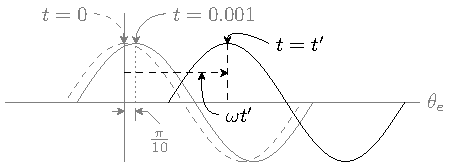
\includegraphics{figRotatingMachPrinciplesMovingWave}
\begin{tikzpicture}
%grid
%\draw[gray] (-\sRo,-\sRo) grid (\sRo,\sRo);
%axis
\draw[gray](-2,0) --(5,0)node[right]{$\theta_e$}; %axis
\draw[gray] (0,-1)--(0,1.5);
\begin{scope}[gray,dashed]
%cosine wave
\draw (0,1) cos (-1,0);
\draw (0,1) cos (1,0);
\draw (2,-1) cos (1,0);
\draw (2,-1) cos (3,0);
\draw[stealth-](0,1) to [out=90,in=0]++(-0.5,0.5)node[left]{$t=0$};
\end{scope}
%
\begin{scope}[gray,xshift=0.2 cm]
%cosine wave
\draw (0,1) cos (-1,0);
\draw (0,1) cos (1,0);
\draw (2,-1) cos (1,0);
\draw (2,-1) cos (3,0);
\draw[dotted](0,0)--(0,1);
\draw[stealth-](0,1) to [out=90,in=180]++(0.5,0.5)node[right]{$t=0.001$};
%delay
\draw(0,-0.1)--++(0,-0.2);
\draw[stealth-](-0.2,-0.15)--++(-0.2,0);
\draw[stealth-](0,-0.15)--++(0.2,0)--++(0.2,-0.2)node[below]{$\tfrac{\pi}{10}$};
\end{scope}
%
\begin{scope}[xshift=1.75 cm]
%cosine wave
\draw (0,1) cos (-1,0);
\draw (0,1) cos (1,0);
\draw (2,-1) cos (1,0);
\draw (2,-1) cos (3,0);
\draw[stealth-](0,1) to [out=90,in=150]++(0.7,0)node[right]{$t=t'$};
\draw[dashed,black](0,1)--(0,0);
\end{scope}
\draw[dashed,-stealth](0,0.5)--++(1.75,0)coordinate[pos=0.75](finalPlace);
\draw[stealth-](finalPlace) to [out=-90,in=180] (1.6,-0.2)node[right]{$\omega t'$};
\end{tikzpicture}
\caption{حرکت کرتی موج۔}
\label{شکل_گھومتے_مشین_حرکت_کرتی_موج}
\end{figure}
ہم دیکھتے ہیں کہ موج کی چوٹی صفر برقی زاویہ پر ہے۔اسے شکل \حوالہ{شکل_گھومتے_مشین_حرکت_کرتی_موج} میں ہلکی سیاہی میں نقطہ داو لکیر سے دکھایا گیا ہے۔ہم اس چوٹی کو کچھ وقفے کے بعد دوبارہ دیکھتے ہیں مثلاً \عددیء{t=0.001} سیکنڈ کے بعد۔
\begin{align*}
&\theta-\omega t =0\\
&\theta -\omega \times 0.001=0\\
&\theta =0.001 \omega =0.001 \times 2 \times \pi \times 50=\SI{0.3142}{\radian} 
\end{align*}
اب یہ چوٹی \عددیء{0.3142} یا \عددیء{\tfrac{\pi}{10}} برقی ریڈیئن یعنی \عددیء{18\degree} کے برقی زاویہ پر ہے۔اسے  شکل میں ہلکی سیاہی کے ٹھوس لکیر سے دکھایا گیا ہے۔یہ بات واضح ہے کہ مقناطیسی دباو کی موج گھڑی کی اُلٹی سمت یعنی زاویہ بڑھنے کی سمت میں گھوم گئی ہے۔ اسی طرح \عددیء{t=0.002}  پر یہ چوٹی \عددیء{36\degree} برقی زاویہ پر نظر آئے گی۔کسی بھی لمحہ \عددیء{t'} پر بالکل اسی طرح چوٹی کا مقام معلوم کیا جا سکتا ہے جسے شکل میں تیز سیاہی کے ٹھوس لکیر سے دکھایا گیا ہے۔
\begin{align*}
&\theta-\omega t' =0\\
&\theta =\omega t'
\end{align*}
اس مساوات سے یہ واضح ہے کہ چوٹی کا مقام متعین کرنے والا زاویہ بتدریج بڑھتا رہتا ہے۔اس مساوات سے ہم ایک مکمل \عددیء{2\pi} برقی زاویہ کے چکر کا وقت \عددیء{T} حاصل کر سکتے ہیں یعنی
\begin{gather}
\begin{aligned}\label{مساوات_گھومتے_مشین_دوری_وقفہ}
t&=\frac{\theta}{\omega}\\
T&=\frac{2\pi}{2\pi f}=\frac{1}{f}
\end{aligned}
\end{gather}
اگر برقی رو کی تعدد \عددیء{50} ہو تو یہ مقناطیسی دباو کی موج ہر \عددیء{\tfrac{1}{50}=0.02} سیکنڈ میں ایک مکمل برقی چکر کاٹتی ہے یعنی یہ ایک سیکنڈ میں \عددیء{50} برقی چکر کاٹتی ہے۔

اس مثال میں برقی زاویہ کی بات ہوتی رہی۔ دو قطب کی آلوں میں برقی زاویہ \عددیء{\theta_e}  اور میکانی زاویہ \عددیء{\theta_m} برابر ہوتے ہیں۔ لہٰذا اگر دو قطب کی آلوں کی بات کی جائے تو مساوات \حوالہ{مساوات_گھومتے_مشین_دوری_وقفہ}  کے تحت ایک سیکنڈ میں مقناطیسی دباو کی موج \عددیء{f} برقی یا میکانی چکر کاٹے گی جہاں \عددیء{f} برقی رو کی تعدد ہے اور اگر \عددیء{P} قطب رکھنے والی آلوں کی بات کی جائے تو چونکہ
\begin{align}
\theta_e=\frac{P}{2} \theta_m
\end{align}
لہٰذا ایسے آلوں میں یہ مقناطیسی دباو کی موج ایک سیکنڈ میں \عددیء{f} مقناطیسی چکر یعنی \عددیء{\tfrac{2}{P}f} میکانی شکر کاٹے گی۔

اگر ہم برقی رو کی تعدد کو \عددیء{f_e} سے ظاہر کریں، مقناطیسی دباو کی موج کی چوٹی کے برقی زاویہ کو  \عددیء{\theta_e} اور اس کے میکانی زاویہ کو \عددیء{\theta_m} سے ظاہر کریں اور اسی طرح اسی مقناطیسی دباو کی موج کے گھومنے کی رفتار کو \عددیء{\omega_e} یا \عددیء{\omega_m} سے ظاہر کریں تو
\begin{gather}
\begin{aligned}\label{مساوات_گھومتے_مشین_برقی_میکانی_رفتار_تعلق}
\omega_m&=\frac{2}{P} \omega_e \quad \si{\radian / \second}\\
f_m&=\frac{2}{P} f_e \quad \si{\hertz}\\
n&=\frac{120 f_e}{P} \quad \textup{rpm}
\end{aligned}
\end{gather}
\عددیء{\omega_e} اس موج کی معاصر رفتار  برقی زاویہ فی سیکنڈ میں ہے جبکہ  \عددیء{\omega_m} یہی معاصر رفتار میکانی زاویہ فی سیکنڈ میں ہے۔اسی طرح \عددیء{f_e} اس موج کی برقی  معاصر رفتار برقی ہرٹز میں اور \عددیء{f_m} اس کی میکانی معاصر رفتار\فرہنگ{معاصر رفتار}\حاشیہب{synchronous speed}\فرہنگ{synchronous speed} میکانی ہرٹز میں ہے۔برقی معاصر رفتار \عددیء{f_e}  ہرٹز ہونے کا مطلب یہ ہے کہ ایک سیکنڈ میں یہ موج \عددیء{f_e} برقی چکر کا فاصلہ طے کرے گی جہاں ایک برقی چکر دو قطب کا فاصلہ یعنی \عددیء{2\pi}  ریڈیئن کا زاویہ ہے۔اسی طرح میکانی معاصر رفتار \عددیء{f_m} ہرٹز ہونے کا مطلب ہے کہ یہ موج ایک سیکنڈ میں \عددیء{f_m} میکانی چکر کا فاصلہ طے کرے گی۔ایک میکانی چکر عام زندگی میں ایک چکر کو ہی کہتے ہیں۔ اس مساوات میں \عددیء{n} میکانی چکر فی منٹ\فرہنگ{rpm}\حاشیہب{rpm, rounds per minute}  کو ظاہر کرتے ہیں۔یہ مساوات \اصطلاح{معاصر رفتار}\فرہنگ{معاصر رفتار}\فرہنگ{synchronous speed} کی مساوات ہے۔

یہاں اس بات کا ذکر کرنا ضروری ہے کہ ہم \عددیء{q} دور کی لپٹی مشین جس کے لچھے \عددیء{\tfrac{2\pi}{q}} برقی زاویہ پر رکھے گئے ہوں اور جن میں \عددیء{q} دور کی برقی رو  ہو، ایک ہی سمت میں گھومتی مقناطیسی دباو کی موج کو جنم دیتی ہے جیسے ہم نے تین دور کی مشین کے لئے دیکھا۔ مزید یہ کہ اس موج کا حیطہ کسی ایک لچھے سے پیدا مقناطیسی دباو کے حیطہ  کے \عددیء{\tfrac{q}{2}}  گنا ہو گا اور اس کے گھومنے کی رفتار \عددیء{\omega_e=2\pi f} برقی ریڈیئن فی سیکنڈ ہو گی۔

\جزوحصہ{تین دور کی لپٹی مشین کا ترسیمی تجزیہ}
شکل \حوالہ{شکل_گھومتے_مشین_تین_دور_کے_لئے_لپٹی}  میں تین دور کی لپٹی مشین دکھائی گئی ہے۔ اس میں مثبت برقی رو کی سمتیں بھی دکھائی گئی ہیں، مثلاً \عددیء{a} شگاف میں برقی رو صفحہ سے عمودی سمت میں باہر جانب کو ہے اور یہ بات نقطہ سے واضح کی گئی ہے۔ اسی طرح \عددیء{a'} شگاف میں برقی دباو صفحہ سے عمودی سمت میں اندر کی جانب کو ہے اور یہ بات صلیب کے نشان سے واضح کی گئی ہے۔ اگر برقی رو مثبت ہو تو اس کی یہی سمت ہو گی اور اس سے پیدا مقناطیسی دباو \عددیء{\سمتیہ{\tau}_a} صفر زاویہ کی جانب ہو گا جیسے شکل میں دکھایا گیا ہے۔ لچھے میں برقی رو سے پیدا مقناطیسی دباو کی سمت دائیں ہاتھ کے قانون سے معلوم کی جا سکتی ہے۔ اب اگر اسی لچھے میں برقی رو منفی ہو تو اس کا مطلب ہے کہ برقی رو اُلٹ سمت میں ہے۔ یعنی اب برقی رو \عددیء{a} شگاف میں صفحہ کے عمودی سمت میں اندر کی جانب ہے اور \عددیء{a'} شگاف میں یہ صفحہ کے عمودی سمت میں باہر کی جانب کو ہے۔ لہٰذا اس برقی رو سے پیدا مقناطیسی دباو بھی پہلے سے اُلٹ سمت میں ہو گی یعنی یہ شکل میں دیئے گئے  \عددیء{\سمتیہ{\tau}_a}  کے بالکل اُلٹ سمت میں ہو گی۔ اس تذکرہ کا بنیادی مقصد یہ تھا کہ آپ پر یہ بات واضح ہو جائے کہ برقی رو کے منفی ہونے سے اس سے پیدا مقناطیسی دباو کی سمت اُلٹ ہو جاتی ہے۔

اس شکل میں لچھوں میں برقی رو اور مقناطیسی دباو یہ ہیں
\begin{gather}
\begin{aligned}\label{مساوات_گھومتے_مشین_تین_دور_برقی_رو}
i_a&=I_0 \cos \omega t\\
i_b&=I_0 \cos (\omega t-120\degree)\\
i_c&=I_0 \cos (\omega t+120\degree)
\end{aligned}
\end{gather}
%
\begin{gather}
\begin{aligned}\label{مساوات_گھومتے_مشین_تین_دور_دباو}
\tau_a&=k_w \frac{4}{\pi}\frac{N i_a}{2}=k_w \frac{4}{\pi}\frac{N I_0}{2} \cos \omega t=\tau_0 \cos \omega t\\
\tau_b&=k_w \frac{4}{\pi}\frac{N i_b}{2}=k_w \frac{4}{\pi}\frac{N I_0}{2} \cos (\omega t-120\degree)=\tau_0 \cos (\omega t-120\degree)\\
\tau_c&=k_w \frac{4}{\pi}\frac{N i_c}{2}=k_w \frac{4}{\pi}\frac{N I_0}{2} \cos (\omega t+120\degree)=\tau_0 \cos (\omega t+120\degree)
\end{aligned}
\end{gather}
جبکہ ان کے مثبت سمتیں شکل میں دیئے گئے ہیں۔ اب ہم مختلف اوقات پر ان مقداروں کا حساب لگاتے ہیں اور ان کا کُل مجموعی مقناطیسی دباو حل کرتے ہیں۔

لمحہ \عددیء{t=0} پر ان مساوات سے ملتا ہے۔
\begin{gather}
\begin{aligned}
i_a&=I_0 \cos 0=I_0\\
i_b&=I_0 \cos (0-120\degree)=-0.5 I_0\\
i_c&=I_0 \cos (0+120\degree)=-0.5 I_0
\end{aligned}
\end{gather}
%
\begin{gather}
\begin{aligned}
\tau_a&=\tau_0 \cos 0=\tau_0\\
\tau_b&=\tau_0 \cos (0-120\degree)=-0.5 \tau_0\\
\tau_c&=\tau_0 \cos (0+120\degree)=-0.5 \tau_0
\end{aligned}
\end{gather}
یہاں رکھ کر ذرا غور کریں۔اس لمحہ پر  \عددیء{i_a} مثبت ہے جبکہ \عددیء{i_b} اور \عددیء{i_c} منفی ہیں۔ لہٰذا \عددیء{i_a}  اُسی سمت میں ہے جو شکل  \حوالہ{شکل_گھومتے_مشین_تین_دور_کے_لئے_لپٹی} میں \عددیء{a} اور \عددیء{a'} شگافوں میں نقطے اور صلیب سے  دکھائے  گئے ہیں جبکہ  \عددیء{i_b} اور \عددیء{i_c} شکل میں دیئے گئے سمتوں کے اُلٹ ہیں۔ ان تینوں برقی رو کی اس لمحہ پر درست سمتیں شکل \حوالہ{شکل_گھومتے_مشین_لمحہ_صفر_پر_کل_دباو}  میں دکھائی گئی ہیں۔اس شکل میں تینوں مقناطیسی دباو بھی دکھائے گئے ہیں۔
\begin{figure}
\centering
%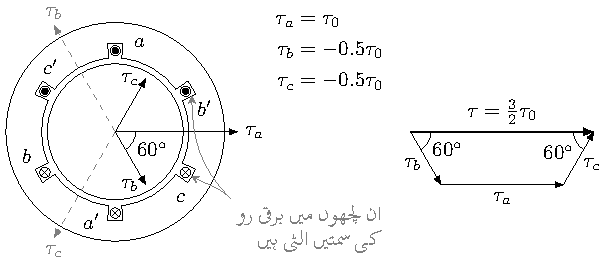
\includegraphics{figRotatingMachPrinciplesThreePhaseFluxAtTimeZero}
\begin{tikzpicture}
%grid
%\draw[gray] (-\sRo,-\sRo) grid (\sRo,\sRo);
\pgfmathsetmacro{\shiftX}{5cm}
\stator{6}{30}
\slotDot{90,30,150}
\slotCross{-30,-90,-150}
\draw (0,0) circle (\rR);
%
%\slotName{45/a_1/,-45/a_1'/below,135/a_2'/,-135/a_2/below}
\draw (90-15:\sRi+1.25*\delR)node[]{$a$};
\draw (270-15:\sRi+1.25*\delR)node[]{$a'$};
\draw (210-15:\sRi+1.25*\delR)node[]{$b$};
\draw (30-15:\sRi+1.25*\delR)node[]{$b'$};
\draw (-30-15:\sRi+1.25*\delR)node[]{$c$};
\draw (150-15:\sRi+1.25*\delR)node[]{$c'$};
%
\draw[-latex](0,0)--(0:1.8*\rR)node[right]{$\tau_a$};
\draw[gray,dashed,-latex](0,0)--(120:1.8*\rR)node[above]{$\tau_b$};
\draw[gray,dashed,-latex](0,0)--(-120:1.8*\rR)node[below]{$\tau_c$};
\draw[-latex](0,0)--(-60:0.9*\rR)node[left]{$\tau_b$};
\draw[-latex](0,0)--(60:0.9*\rR)node[left]{$\tau_c$};
\draw (-60:0.3*\rR) arc (-60:0:0.3*\rR);
\draw node at (-25:0.6*\rR){$60\degree$};
%text
\draw node[right] at (2.2*\rR,1.2*\rR){$\begin{aligned}
\tau_a&=\tau_0\\
\tau_b&=-0.5 \tau_0\\
\tau_c&=-0.5 \tau_0
\end{aligned}$};
%
\draw[gray,stealth-] (-30:\sRi cm+\delR cm )++(0,0) to [out=-30,in=135]++(-30:0.6*\sRi)coordinate(reversedText);
\draw[gray,stealth-] (30:\sRi cm+\delR cm )++(0,-0.15cm) to [out=-90,in=135](reversedText)node[below right,align=right]{\RL{ان لچھوں میں برقی رو} \\ \RL{ کے رخ ایک دوسرے}\\  \RL{کے الٹ ہیں}};
%=============
\begin{scope}[xshift=\shiftX]
\draw[-latex](0,0)--++(-60:0.9*\rR)node[pos=0.6,left]{$\tau_b$}coordinate(tipB);
\draw[-latex](tipB)--++(0:1.8*\rR)node[pos=0.5,below]{$\tau_a$}coordinate(tipA);
\draw[-latex](tipA)--++(60:0.9*\rR)node[pos=0.4,right]{$\tau_c$}coordinate(tipC);
\draw[-latex,thick](0,0)--(tipC)node[pos=0.5,above]{$\tau=\tfrac{3}{2} \tau_0$};
\draw (-60:0.3*\rR) arc (-60:0:0.3*\rR);
\draw node at (-25:0.6*\rR){$60\degree$};
\draw (tipC)++(180:0.3*\rR) arc (180:240:0.3*\rR);
\draw (tipC)++(210:0.6*\rR)node{$60\degree$};
\end{scope}
\end{tikzpicture}
\caption{ لمحہ \عددیء{t_0=0} پر برقی رو اور مقناطیسی دباو۔}
\label{شکل_گھومتے_مشین_لمحہ_صفر_پر_کل_دباو}
\end{figure}

کل مقناطیسی دباو با آسانی بذریعہ ترسیم،  مجموعہ سمتیات سے  معلوم کیا جا سکتا ہے یا پھر الجبرا کے ذریعہ ایسا کیا جا سکتا ہے۔
\begin{gather}
\begin{aligned}
\kvec{\tau}_a&=\tau_0 \ax\\
\kvec{\tau}_b&=0.5 \tau_0 \left[\cos (60\degree) \ax-\sin (60\degree)\ay \right]\\
\kvec{\tau}_c&=0.5 \tau_0 \left[\cos (60\degree) \ax+\sin (60\degree)\ay \right]
\end{aligned}
\end{gather}
%
\begin{align}
\kvec{\tau}=\kvec{\tau}_a+\kvec{\tau}_b+\kvec{\tau}_c=\frac{3}{2} \tau_0 \ax
\end{align}
کل مقناطیسی دباو ایک لچھے کے مقناطیسی دباو کے ڈیڑھ گنا ہے اور یہ صفر زاویہ پر ہے۔ اب ہم گھڑی کو چلنے دیتے ہیں اور کچھ لمحے بعد \عددیء{t_1} پر دوبارہ یہی سب حساب لگاتے ہیں۔ چونکہ مساوات \حوالہ{مساوات_گھومتے_مشین_تین_دور_برقی_رو}  اور مساوات \حوالہ{مساوات_گھومتے_مشین_تین_دور_دباو}  میں متغیرہ \عددیء{t} کے بجائے \عددیء{\omega t} کا استعمال زیادہ آسان ہے لہٰذا ہم لمحہ \عددیء{t_1} کو یوں چنتے ہیں کہ \عددیء{\omega t_1=30\degree}  کے برابر ہو۔ ایسا کرنے سے ہمیں یہ دو مساواتوں سے حاصل ہوتا ہے۔
\begin{gather}
\begin{aligned}
i_a&=I_0 \cos 30\degree=\frac{\sqrt{3}}{2} I_0\\
i_b&=I_0 \cos (30\degree-120\degree)=0\\
i_c&=I_0 \cos (30\degree+120\degree)=-\frac{\sqrt{3}}{2} I_0
\end{aligned}
\end{gather}
%
\begin{gather}
\begin{aligned}
\tau_a&=\tau_0 \cos 30\degree=\frac{\sqrt{3}}{2} \tau_0\\
\tau_b&=\tau_0 \cos (30\degree-120\degree)=0\\
\tau_c&=\tau_0 \cos (30\degree+120\degree)=-\frac{\sqrt{3}}{2} \tau_0
\end{aligned}
\end{gather}
%
\begin{figure}
\centering
%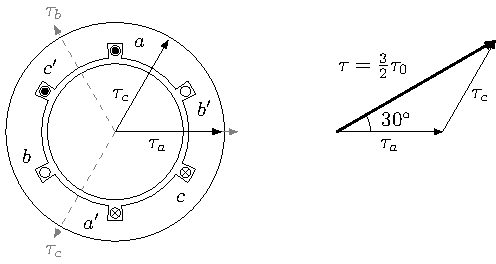
\includegraphics{figRotatingMachPrinciplesThreePhaseFluxAtTimeThirtyDegrees}
\begin{tikzpicture}
%grid
%\draw[gray] (-\sRo,-\sRo) grid (\sRo,\sRo);
\pgfmathsetmacro{\shiftX}{5cm}
\stator{6}{30}
\slotDot{90,150}
\slotCross{-30,-90}
\slotEmptyCircle{30,210}
\draw (0,0) circle (\rR);
%
%\slotName{45/a_1/,-45/a_1'/below,135/a_2'/,-135/a_2/below}
\draw (90-15:\sRi+1.25*\delR)node[]{$a$};
\draw (270-15:\sRi+1.25*\delR)node[]{$a'$};
\draw (210-15:\sRi+1.25*\delR)node[]{$b$};
\draw (30-15:\sRi+1.25*\delR)node[]{$b'$};
\draw (-30-15:\sRi+1.25*\delR)node[]{$c$};
\draw (150-15:\sRi+1.25*\delR)node[]{$c'$};
%
\draw[gray,-latex](0,0)--(0:1.8*\rR);
\draw[gray,dashed,-latex](0,0)--(120:1.8*\rR)node[above]{$\tau_b$};
\draw[gray,dashed,-latex](0,0)--(-120:1.8*\rR)node[below]{$\tau_c$};
\draw[-latex](0,0)--(0:1.8*0.866*\rR)node[pos=0.4,below]{$\tau_a$};
%\draw[-latex](0,0)--(-60:0.9*\rR)node[left]{$\tau_b$};
\draw[-latex](0,0)--(60:1.8*0.866*\rR)node[pos=0.4,left]{$\tau_c$};
%=============
\begin{scope}[xshift=0.75*\shiftX]
\draw[-latex](0,0)--++(0:1.8*0.866*\rR)node[pos=0.5,below]{$\tau_a$}coordinate(tipA);
\draw[-latex](tipA)--++(60:1.8*0.866*\rR)node[pos=0.4,right]{$\tau_c$}coordinate(tipC);
\draw[-latex,thick](0,0)--(tipC)node[pos=0.5,above left]{ $\tau=\tfrac{3}{2}\tau_0$};
*
%\draw(tipA)++(60:0.2*\rR) arc (60:180:0.2*\rR);
%\draw (tipA)++(120:0.4*\rR)node{$120\degree$};
\draw(0:0.5*\rR) arc (0:30:0.5*\rR);
\draw node at (12:0.9*\rR){$30\degree$};
\end{scope}
\end{tikzpicture}
\caption{ لمحہ \عددیء{\omega t_1=30\degree} پر برقی رو اور مقناطیسی دباو۔}
\label{شکل_گھموتے_مشین_وقت_تیس_پر_دباو}
\end{figure}
یہ شکل \حوالہ{شکل_گھموتے_مشین_وقت_تیس_پر_دباو}  میں دکھایا گیا ہے۔کل مقناطیسی دباو کا طول \عددیء{\tau} کو تکون کے ذریعہ یوں حل کیا جا سکتا ہے۔ اسی طرح اس کا زاویہ بھی اسی سے حاصل ہوتا ہے۔ یعنی
\begin{align}
\tau=\sqrt{\tau_a^2+\tau_c^2-2 \tau_a \tau_c \cos 120\degree}=\frac{3}{2}\tau_0
\end{align}
اور چونکہ اس تکون کے دو اطراف برابر ہیں لہٰذا اس کے باقی دو زاویہ بھی برابر اور \عددیء{30\degree} ہیں۔

ہم دیکھتے ہیں کہ کُل مقناطیسی دباو جو پہلے صفر زاویہ پر تھا اب وہ \عددیء{30\degree}  کے زاویہ پر ہے یعنی وہ گھڑی کے اُلٹ سمت گھوم گیا ہے۔ اگر ہم اسی طرح \عددیء{\omega t =40\degree} پر دیکھیں تو ہمیں کُل مقناطیسی دباو اب بھی \عددیء{\tfrac{3}{2}\tau_0} ہی ملے گا البتہ اب یہ \عددیء{45\degree} کے زاویہ پر ہو گا۔اگر کسی لمحہ جب \عددیء{\omega t=\theta\degree} کے برابر ہو یہ سارا حساب کیا جائے تو کُل مقناطیسی دباو اب بھی \عددیء{\tfrac{3}{2}\tau_0} ہی ملے گا البتہ یہ \عددیء{\theta\degree} کے زاویہ پر ہو گا۔

\حصہ{محرک برقی دباو}
یہاں محرک برقی دباو\حاشیہد{ابتداء میں حرکت سے پیدا ہونے والی برقی دباو کو محرک برقی دباو کہتے تھے۔اب روایتی طور پر کسی بھی طرح پیدا کردہ برقی دباو کو محرک برقی دباو کہتے ہیں۔} کو ایک اور زاویہ سے پیش کیا جاتا ہے۔

\جزوحصہ{بدلتی رو برقی جنریٹر}
شکل \حوالہ{شکل_گھومتے_مشین_بنیادی_بدلتی_رو_جنریٹر}  میں ایک بنیادی \اصطلاح{بدلتی رو جنریٹر}\فرہنگ{جنریٹر!بدلتی رو}\حاشیہب{ac generator}\فرہنگ{generator!ac} دکھایا گیا ہے۔اس کا گھومتا برقی مقناطیس، خلائی درز میں سائن نما مقناطیسی دباو  پیدا کرتا ہے جس سے  درز میں سائن نما کثافتِ مقناطیسی بہاو \عددیء{B}  پیدا ہوتی ہے، یعنی
\begin{figure}
\centering
%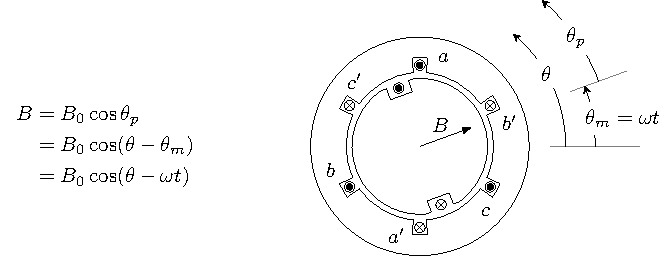
\includegraphics{figRotatingMachPrinciplesBasicACgenerator}
\begin{tikzpicture}
%grid
%\draw[gray] (-\sRo,-\sRo) grid (\sRo,\sRo);
\pgfmathsetmacro{\shiftX}{5cm}
\stator{6}{30}
\slotDot{90,-30,210}
\slotCross{-90,30,150}
\pgfmathsetmacro{\pTheta}{150}
\pgfmathsetmacro{\pY}{0.2}
\pgfmathsetmacro{\rTilt}{20}
\rotor{2}{\rTilt}
%dot on rotot
\draw (90+\rTilt:\rR-\pX) circle (2.5pt);
\draw[fill] (90+\rTilt:\rR-\pX) circle (1.5pt);
%CROSS on rotor
\draw (\rTilt-90:\rR-\pX) circle (2.5pt);
\draw (\rTilt-90:\rR-\pX)++(45:2.2pt)--++(-135:4.4pt);
\draw (\rTilt-90:\rR-\pX)++(-45:2.2pt)--++(135:4.4pt);
%mmf vector and angles
\draw[-latex] (0,0)--(\rTilt:0.8*\rR)node[above,pos=0.4]{$B$};
\draw[gray](0:1.2*\sRo)--++(0:1.5cm);
\draw[gray](\rTilt:1.2*\sRo cm +0.5cm)--++(\rTilt:1cm);
%
\draw[-stealth] (0:1.2*\sRo cm +0.75 cm)  arc (0:\rTilt:1.2*\sRo cm +0.75 cm);
\draw node[right,fill=white] at (\rTilt/2:1.2*\sRo cm+0.5 cm){$\theta_m=\omega t$}; 
%
\draw[-stealth] (\rTilt:1.2*\sRo cm +1 cm)  arc (\rTilt:\rTilt+30:1.2*\sRo cm +1 cm);
\draw node[fill=white] at (\rTilt+15:1.2*\sRo+1){$\theta_p$};
%
\draw[-stealth] (0:1.2*\sRo cm +0.25 cm)  arc (0:\rTilt+30:1.2*\sRo cm +0.25 cm);
\draw node[fill=white] at (\rTilt/2+20:1.2*\sRo cm+0.25 cm){$\theta$};
%\slotName{45/a_1/,-45/a_1'/below,135/a_2'/,-135/a_2/below}
\draw (90-15:\sRi+1.25*\delR)node[]{$a$};
\draw (270-15:\sRi+1.25*\delR)node[]{$a'$};
\draw (210-15:\sRi+1.25*\delR)node[]{$b$};
\draw (30-15:\sRi+1.25*\delR)node[]{$b'$};
\draw (-30-15:\sRi+1.25*\delR)node[]{$c$};
\draw (150-15:\sRi+1.25*\delR)node[]{$c'$};
%text
\draw node[left] at (-2*\sRo,0){$
\begin{aligned}
B&=B_0 \cos \theta_p\\
&=B_0 \cos(\theta-\theta_m)\\
&=B_0 \cos (\theta-\omega t)
\end{aligned}
$};
\end{tikzpicture}
\caption{بنیادی بدلتی رو جنریٹر۔}
\label{شکل_گھومتے_مشین_بنیادی_بدلتی_رو_جنریٹر}
\end{figure}
%
\begin{align}
B=B_0 \cos \theta_p
\end{align}
یہ مقناطیس \عددیء{\omega} زاویاتی رفتار سے گھوم رہا ہے۔یوں اگر ابتدائی لمحہ  \عددیء{t=0} پر  یہ \عددیء{a} لچھے کی سمت یعنی ہلکی سیاہی کی  اُفقی لکیر کی سمت میں ہو تو لمحہ  \عددیء{t} پر یہ گھوم کر زاویہ \عددیء{\theta_m=\omega t} پر ہو گا۔اس طرح یہی مساوات  یوں بھی لکھا جا سکتا ہے۔
\begin{gather}
\begin{aligned}\label{مساوات_گھومتے_مشین_کثافت_بالمقابل_زاویہ}
B&=B_0 \cos (\theta-\theta_m)\\
&=B_0 \cos (\theta -\omega t)
\end{aligned}
\end{gather}
%
\begin{figure}
\centering
%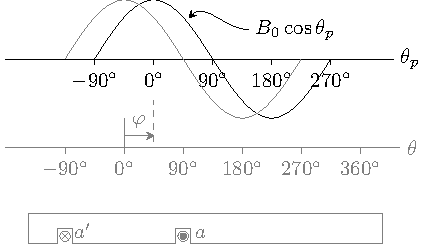
\includegraphics{figRotatingMachPrinciplesFluxCuttingSingleStatorCoil}
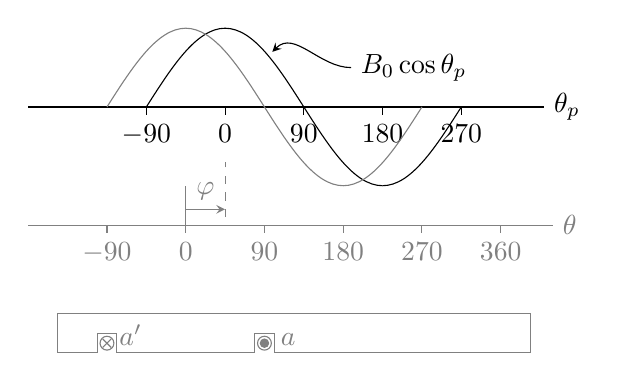
\begin{tikzpicture}
%grid
%\draw[gray,thick] (-2*\sRo,-2*\sRo) grid (2*\sRo,3*\sRo);
%\draw[gray,thin,xstep=0.1,ystep=0.1] (-2*\sRo,-2*\sRo) grid (2*\sRo,3*\sRo);
%
%\pgfmathsetmacro{\j}{0.25}
\pgfmathsetmacro{\shiftY}{2.5}
%
\begin{scope}[gray]
%\newcommand{\dotLinear}[1]{
\pgfmathsetmacro{\delSlotX}{3.5}
\foreach \x in {90}{
\pgfmathsetmacro{\x}{\x/90}
\draw(\x cm-\delSlotX pt,-\delSlotX pt)--++(0,2*\delSlotX pt)--++(2*\delSlotX pt,0)--++(0,-2*\delSlotX pt);
\draw (\x,0) circle (2.5pt);
\draw[fill] (\x,0) circle (1.5pt); }
\draw node[shift={(0.3,0.05)}] at (1,0){$a$};
%====================================
%CROSS LINEAR
%\crossLinear{comma separated x-locations}
\pgfmathsetmacro{\delSlotX}{3.5}
\foreach \x in {-90}{
\pgfmathsetmacro{\x}{\x/90}
\draw(\x cm-\delSlotX pt,-\delSlotX pt)--++(0,2*\delSlotX pt)--++(2*\delSlotX pt,0)--++(0,-2*\delSlotX pt);
\draw (\x,0) circle (2.5pt);
\draw (\x,0)++(45:2.2pt)--++(-135:4.4pt);
\draw (\x,0)++(-45:2.2pt)--++(135:4.4pt);  }
\draw node[shift={(0.3,0.1)}] at (-1,0){$a'$};
%==================================
%SLOT SEGMENT
%\slotSegment{comma separated xStart/xEnd locations}
\pgfmathsetmacro{\delSlotX}{3.5}
\foreach \xStart/\xEnd in {-90/90,90/360}{
\pgfmathsetmacro{\xStart}{\xStart/90}
\pgfmathsetmacro{\xEnd}{\xEnd/90}
\draw(\xStart cm+\delSlotX pt,-\delSlotX pt) --(\xEnd cm -\delSlotX pt,-\delSlotX pt); }
%
%this is used after \slotSegment to draw the top cover
%\newcommand{\slotTop}[1]{
\foreach \xStart/\xEnd in {-90/360}{
\pgfmathsetmacro{\xStart}{\xStart/90}
\pgfmathsetmacro{\xEnd}{\xEnd/90}
\draw (\xStart cm-\delSlotX pt,-\delSlotX pt)--++(-0.5 cm,0)--++(0,0.5)--++(\xEnd cm-\xStart cm+1 cm ,0)--++(0,-0.5)--(\xEnd cm-\delSlotX pt,-\delSlotX pt); }
%================================
%axis
\draw (-180/90, 1.5)--++(600/90,0)node[right]{$\theta$};
\draw(0,1.5)--++(0,0.5);
\foreach \x in {-90,0,90,180,270,360}{
\draw (\x/90,1.5)--++(0,-0.1)node[below]{$\x\degree$}; }
%
\draw[dashed](0.5,1.5+0.1)--++(0,0.7);
\draw[-stealth](0,1.5+0.2)--++(0.5,0)node[above,pos=0.5]{$\varphi$};
%
\end{scope}
%
\begin{scope}[xshift=0.5 cm,yshift=3 cm ]
%axis
\draw (-225/90, 0)--++(590/90,0)node[right]{$\theta_p$};
\foreach \x in {-90,0,90,180,270}{
\draw (\x/90,0)--++(0,-0.1)node[below]{$\x\degree$}; }
%cosine DARK
\draw (0,1) cos (-1,0);
\draw (0,1) cos (1,0);
\draw(2,-1) cos (1,0);
\draw (2,-1) cos (3,0);
%cosine LIGHT
\draw[gray] (-0.5,1) cos (-1.5,0);
\draw[gray] (-0.5,1) cos (0.5,0);
\draw[gray](1.5,-1) cos (0.5,0);
\draw[gray] (1.5,-1) cos (2.5,0);
%text
\draw[stealth-] (0.6,0.7) to [out=45,in=180] ++(1,-0.2) node[right] {$B_0 \cos \theta_p$};
\end{scope}
\end{tikzpicture}
\caption{لچھے میں سے گزرتا مقناطیسی بہاو۔}
\label{شکل_گھومتے_مشین_لچھے_سے_گزرتی_بیاو}
\end{figure}
%
شکل \حوالہ{شکل_گھومتے_مشین_لچھے_سے_گزرتی_بیاو}  میں \عددیء{B} کو زاویہ \عددیء{\theta} اور \عددیء{\theta_p}  کے ساتھ ترسیم کیا گیا ہے۔ اسی ترسیم میں لچھا \عددیء{a} بھی دکھایا گیا ہے۔اس شکل میں ہلکی سیاہی سے لمحہ \عددیء{t=0} پر \عددیء{B} دکھایا گیا ہے جب گھومتے برقی مقناطیس کا محور اور اس لچھے کا محور ایک ہی سمت میں ہوتے ہیں جبکہ کالی سیاہی میں اسی \عددیء{B} کو کسی  بھی لمحہ \عددیء{t} پر دکھایا گیا ہے۔اس لمحہ پر برقی مقناطیس کے محور اور لچھے کے محور کے مابین \عددیء{\vartheta} زاویہ ہے۔ یہ زاویہ برقی مقناطیس کے گھومنے کی رفتار \عددیء{\omega} پر منحصر ہے یعنی
\begin{align}
\vartheta=\omega t
\end{align}
لمحہ \عددیء{t=0} پر لچھے میں سے زیادہ سے زیادہ مقناطیسی بہاو گزر رہی ہے۔ اگر خلائی درز بہت باریک ہو، تو اس کے اندر اور باہر جانب کے رداس تقریباً یکساں ہوں گے۔ برقی مقناطیس کے محور سے اس خلائی درز تک کا اوسط رداسی فاصلہ اگر \عددیء{\rho} ہو اور برقی مقناطیس کا دھرے\فرہنگ{دھرا}\حاشیہب{axle}\فرہنگ{axle} کی سمت میں محوری لمبائی\فرہنگ{محور}\حاشیہب{axial length} \عددیء{l} ہو تو اس لچھے میں وہی مقناطیسی بہاو ہو گا جو اس خلائی درز میں  \عددیء{-\tfrac{\pi}{2} < \theta < \tfrac{\pi}{2}}  کے مابین ہے۔ لمحہ \عددیء{t=0} پر اسے یوں معلوم کیا جا سکتا ہے
\begin{gather}
\begin{aligned}\label{مساوات_گھومتے_مشین_قطب_پر_بہاو}
\phi_a(0)&=\int_{-\frac{\pi}{2}}^{+\frac{\pi}{2}} \kvec{B} \cdot \dif \kvec{S}\\
&=\int_{-\frac{\pi}{2}}^{+\frac{\pi}{2}} (B_0 \cos \theta_p)(l \rho \dif \theta_p)\\
&=B_0 l \rho \left. \sin \theta_p \right|_{-\frac{\pi}{2}}^{+\frac{\pi}{2}}\\
&=2 B_0 l \rho\\
&=\phi_0
\end{aligned}
\end{gather}
جہاں آخر میں  \عددیء{\phi_a(0)} کو \عددیء{\phi_0} کہا گیا ہے۔ یہی حساب اگر لمحہ \عددیء{t} پر کی جائے تو کچھ یوں ہو گا۔
\begin{gather}
\begin{aligned}
\phi_a(t)&=\int_{-\frac{\pi}{2}-\vartheta}^{+\frac{\pi}{2}-\vartheta} \kvec{B} \cdot \dif \kvec{S}\\
&=\int_{-\frac{\pi}{2}-\vartheta}^{+\frac{\pi}{2}-\vartheta} (B_0 \cos \theta_p)(l \rho \dif \theta_p)\\
&=B_0 l \rho \left. \sin \theta_p \right|_{-\frac{\pi}{2}-\vartheta}^{+\frac{\pi}{2}-\vartheta}\\
&=2 B_0 l \rho \cos \vartheta\\
&=2 B_0 l \rho \cos \omega t
\end{aligned}
\end{gather}
جہاں \عددیء{\vartheta=\omega t} لیا گیا ہے۔اسی مساوات کو یوں بھی حل کیا جا سکتا ہے
\begin{gather}
\begin{aligned}\label{مساوات_گھومتے_مشین_قطبی_بہاو_بالمقابل_وقت}
\phi_a(t)&=\int_{-\frac{\pi}{2}}^{+\frac{\pi}{2}} \kvec{B} \cdot \dif \kvec{S}\\
&=\int_{-\frac{\pi}{2}}^{+\frac{\pi}{2}} (B_0 \cos (\theta-\omega t))(l \rho \dif \theta)\\
&=B_0 l \rho \left. \sin (\theta-\omega t) \right|_{-\frac{\pi}{2}}^{+\frac{\pi}{2}}\\
&=B_0 l \rho \left[\sin \left(\frac{\pi}{2}-\omega t \right )-\sin \left (-\frac{\pi}{2}-\omega t \right) \right]\\
&=2 B_0 l \rho \cos \omega t
\end{aligned}
\end{gather}
اس مرتبہ تکمل زاویہ \عددیء{\theta} کے ساتھ کیا گیا ہے۔ انہیں مساوات \حوالہ{مساوات_گھومتے_مشین_قطب_پر_بہاو}  کی مدد سے یوں لکھا جا سکتا ہے۔
\begin{align}
\phi_a(t)=2 B_0 l \rho \cos \omega t=\phi_0 \cos \omega t
\end{align}
بالکل مساوات  \حوالہ{مساوات_گھومتے_مشین_قطبی_بہاو_بالمقابل_وقت} کی طرح ہم  \عددیء{b} اور \عددیء{c} لچھوں کے لئے  بھی مقناطیسی بہاو کی مساواتیں حل کر سکتے ہیں۔شکل \حوالہ{شکل_گھومتے_مشین_بنیادی_بدلتی_رو_جنریٹر}  میں \عددیء{a} لچھے میں زاویہ \عددیء{-\tfrac{\pi}{2}} سے \عددیء{+\tfrac{\pi}{2}}  تک کا مقناطیسی بہاو گزرتا ہے۔ اس لئے \عددیء{\phi_a(t)}  معلوم کرنے کے لئے مساوات \حوالہ{مساوات_گھومتے_مشین_قطبی_بہاو_بالمقابل_وقت}  میں تکمل کے حدود یہی رکھے گئے تھے۔ اسی شکل سے واضح ہے کہ \عددیء{b} لچھے کے تکمل کے حدود 
\عددیء{+\tfrac{\pi}{6}}  اور \عددیء{+\tfrac{7 \pi}{6}} جبکہ \عددیء{c} کے حدود \عددیء{+\tfrac{5\pi}{6}} اور \عددیء{+\tfrac{11\pi}{6}} ہیں۔یہ زاویے ریڈیئن میں دیئے گئے ہیں۔یوں
\begin{gather}
\begin{aligned}
\phi_b(t)&=\int_{\frac{\pi}{6}}^{\frac{7\pi}{6}} \kvec{B} \cdot \dif \kvec{S}\\
&=\int_{\frac{\pi}{6}}^{\frac{7\pi}{6}} (B_0 \cos (\theta-\omega t))(l \rho \dif \theta)\\
&=B_0 l \rho \left. \sin (\theta-\omega t) \right|_{\frac{\pi}{6}}^{\frac{7\pi}{6}}\\
&=B_0 l \rho \left[\sin \left(\frac{7\pi}{6}-\omega t \right )-\sin \left (\frac{\pi}{6}-\omega t \right) \right]\\
&=2 B_0 l \rho \cos (\omega t-\frac{2\pi}{3})
\end{aligned}
\end{gather}
اور
\begin{gather}
\begin{aligned}
\phi_c(t)&=\int_{\frac{5\pi}{6}}^{\frac{11\pi}{6}} \kvec{B} \cdot \dif \kvec{S}\\
&=\int_{\frac{5\pi}{6}}^{\frac{11\pi}{6}} (B_0 \cos (\theta-\omega t))(l \rho \dif \theta)\\
&=B_0 l \rho \left. \sin (\theta-\omega t) \right|_{\frac{5\pi}{6}}^{\frac{11\pi}{6}}\\
&=B_0 l \rho \left[\sin \left(\frac{11\pi}{6}-\omega t \right )-\sin \left (\frac{5\pi}{6}-\omega t \right) \right]\\
&=2 B_0 l \rho \cos (\omega t+\frac{2\pi}{3})
\end{aligned}
\end{gather}
اگر ایک لچھے کے \عددیء{N} چکر ہوں تو اس میں پیدا برقی دباو کو یوں معلوم کیا جا سکتا ہے۔
\begin{gather}
\begin{aligned}
\lambda_a&=N \phi_a (t)=N \phi_0 \cos \omega t\\
\lambda_b&=N \phi_b (t)=N \phi_0 \cos (\omega t-120\degree)\\
\lambda_c&=N \phi_c (t)=N \phi_0 \cos (\omega t+120\degree)
\end{aligned}
\end{gather}
ان مساوات میں \عددیء{\tfrac{2\pi}{3}} ریڈیئن کو \عددیء{120\degree} لکھا گیا ہے۔ان سے لچھوں میں پیدا امالی برقی دباو کا حساب یوں لگایا جا سکتا ہے۔
\begin{gather}
\begin{aligned}\label{مساوات_گھومتے_مشین_تین_دور_سائن_نما_برقی_دباو_الف}
e_a(t)&=-\frac{\dif \lambda_a}{\dif t}=\omega N \phi_0 \sin \omega t\\
e_b(t)&=-\frac{\dif \lambda_b}{\dif t}=\omega N \phi_0 \sin (\omega t-120\degree)\\
e_c(t)&=-\frac{\dif \lambda_c}{\dif t}=\omega N \phi_0 \sin (\omega t+120\degree)
\end{aligned}
\end{gather}
ان مساوات کو یوں بھی لکھ سکتے ہیں
\begin{gather}
\begin{aligned}\label{مساوات_گھومتے_مشین_تین_دور_سائن_نما_برقی_دباو}
e_a(t)&=\omega N \phi_0 \cos (\omega t -90\degree)\\
e_b(t)&=\omega N \phi_0 \cos (\omega t+150\degree)\\
e_c(t)&=\omega N \phi_0 \cos (\omega t+30\degree)
\end{aligned}
\end{gather}
یہ مساوات تین دوری محرک برقی دباو  کو ظاہر کرتے ہیں جو آپس میں \عددیء{120\degree} زاویہ پر ہیں۔ان سب کا حیطہ \عددیء{E_0} یکساں ہے جہاں
\begin{align}
E_0=\omega N \phi_0
\end{align}
اور ان برقی دباو کی موثر قیمت\فرہنگ{موثر قیمت}\حاشیہب{rms}\فرہنگ{rms}
\begin{align}\label{مساوات_گھومتے_مشین_موثر_دباو}
E_{\textup{موثر}}=\frac{E_0}{\sqrt{2}}=\frac{2\pi f N \phi_0}{\sqrt{2}}=4.44 f N \phi_0
\end{align}
ہو گی۔ چونکہ \عددیء{\phi=B A}ہوتا ہے  لہٰذا یہ مساوات بالکل صفحہ \حوالہصفحہ{مساوات_مقناطیسی_دور_پیدا_دباو_موثر_قیمت} پر دئے مساوات \حوالہ{مساوات_مقناطیسی_دور_پیدا_دباو_موثر_قیمت}  کی طرح ہے۔ 

مساوات \حوالہ{مساوات_گھومتے_مشین_تین_دور_سائن_نما_برقی_دباو}  سائن نما برقی دباو کو ظاہر کرتا ہے۔ اگرچہ اسے  یہ سوچ کر حاصل کیا گیا کہ خلائی درز میں مقناطیسی بہاو صرف برقی مقناطیس کی وجہ سے ہے تاہم برقی دباو کا اس سے کوئی تعلق نہیں کہ خلائی درز میں مقناطیسی بہاو کس طرح وجود میں آئی اور یہ مساوات ان حالات کے لئے بھی درست ہے جہاں یہ مقناطیسی بہاو جنریٹر کے ساکن حصے میں پیدا ہوئی ہو یا ساکن اور حرکت پذیر دونوں حصوں میں پیدا ہوئی ہو۔

مساوات \حوالہ{مساوات_گھومتے_مشین_موثر_دباو}  ہمیں ایک گچھ لچھے میں پیدا برقی دباو دیتی ہے۔ اگر لچھا تقسیم شدہ ہو تو اس کے مختلف شگافوں میں موجود اس لچھے کے حصوں میں برقی دباو ہم قدم نہیں ہوں گے لہٰذا ان سب کا مجموعی برقی دباو ان سب کا حاصل جمع نہیں ہو گا بلکہ اس سے قدرِ کم ہو گا۔ اس مساوات کو ہم ایک پھیلے لچھے کے لئے یوں لکھ سکتے ہیں۔
\begin{align}
E_{\textup{موثر}} =4.44 k_w f N \phi_0
\end{align}
تین دور برقی جنریٹروں کے \عددیء{k_w} کی قیمت \عددیء{0.85} تا \عددیء{0.95} ہوتی ہے۔ یہ مساوات ہمیں ایک دور کی برقی دباو دیتی ہے۔ تین دور برقی جنریٹروں میں ایسے تین لچھوں کے جوڑے ہوتے ہیں اور ان کو \عددیء{Y} یعنی ستارہ نما یا \عددیء{\Delta} یعنی تکونی جوڑا جاتا ہے۔

\جزوحصہ{یک سمتی رو برقی جنریٹر}
ہر گھومنے والا برقی جنریٹر بنیادی طور پر بدلتی رو جنریٹر ہی ہوتا ہے۔ البتہ جہاں یک سمتی برقی دباو\فرہنگ{برقی دباو!یک سمتی}\حاشیہب{DC voltage}\فرہنگ{voltage!DC}  کی ضرورت ہو وہاں مختلف طریقوں سے بدلتی برقی دباو  کو یک سمتی برقی دباو میں تبدیل کیا جاتا ہے۔ ایسا الیکٹرانکس کے ذریعہ جنریٹر کے باہر \اصطلاح{برقیاتی سمت کار}\فرہنگ{سمت کار!برقیاتی}\حاشیہب{rectifier}\فرہنگ{rectifier} کی مدد سے  کیا جا سکتا ہے یا پھر میکانی طریقے سے \اصطلاح{میکانی سمت کار}\فرہنگ{سمت کار!میکانی}\حاشیہب{commutator}\فرہنگ{commutator}  کی مدد سے جنریٹر کے اندر ہی کیا جا سکتا ہے۔ مساوات \حوالہ{مساوات_گھومتے_مشین_تین_دور_سائن_نما_برقی_دباو_الف}  میں دیئے گئے برقی دباو کو یک سمتی برقی دباو میں تبدیل کیا جائے تو یہ شکل \حوالہ{شکل_گھومتے_مشین_ایک_دور_یک_سمتی_برقی_دباو}  کی طرح ہو گا۔
\begin{figure}
\centering
%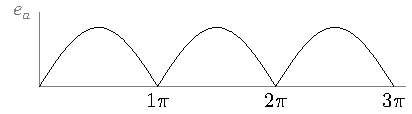
\includegraphics{figRotatingMachPrinciplesFullWaveDCvoltage}
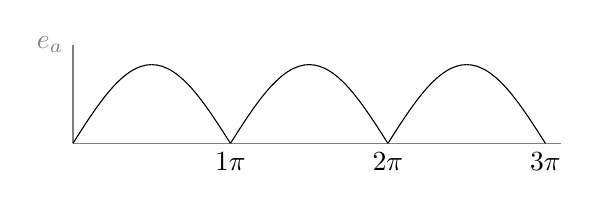
\begin{tikzpicture}
%grid
%\draw[gray,thick] (-2*\sRo,-2*\sRo) grid (2*\sRo,3*\sRo);
%\draw[gray,thin,xstep=0.1,ystep=0.1] (-2*\sRo,-2*\sRo) grid (2*\sRo,3*\sRo);
%

%axis
\draw[gray] (0,0)--(6.2,0);
\draw[gray](0,0)--(0,1.25) node[left]{$e_a$};
%cosine DARK
\draw (1,1) cos (0,0);
\draw (1,1) cos (2,0);
\draw (3,1) cos (2,0);
\draw(3,1) cos (4,0);
\draw (5,1) cos (4,0);
\draw (5,1) cos (6,0);
\draw node[below] at (2,0){$1\pi$};
\draw node[below] at (4,0){$2\pi$};
\draw node[below] at (6,0){$3\pi$};
\end{tikzpicture}
\caption{ایک دور کا یک سمتی برقی دباو۔}
\label{شکل_گھومتے_مشین_ایک_دور_یک_سمتی_برقی_دباو}
\end{figure}
\ابتدا{مثال}
شکل \حوالہ{شکل_گھومتے_مشین_ایک_دور_یک_سمتی_برقی_دباو}  میں یک سمتی برقی دباو دکھائی گئی ہے۔اس یک سمتی برقی دباو کی اوسط قیمت حاصل کریں۔

حل:
\begin{align*}
E_{\textup{اوسط}}=\frac{1}{\pi} \int_{0}^{\pi} \omega N \phi_0 \sin \omega t \dif \,(\omega t)=\frac{2 \omega N \phi_0}{\pi}
\end{align*}
\انتہا{مثال}
یک سمتی برقی جنریٹر پر باقاعدہ تبصرہ کتاب کے باب  میں کیا جائے گا۔

\حصہ{ہموار قطب مشینوں میں قوت مروڑ}
اس حصے میں ہم ایک کامل مشین میں \اصطلاح{قوت مروڑ}\فرہنگ{قوت مروڑ}\حاشیہب{torque}\فرہنگ{torque} کا حساب لگائیں گے۔ ایسا دو طریقوں سے کیا جا سکتا ہے۔ ہم مشین کو دو مقناطیس سمجھ کر ان کے مابین قوتِ کشش، قوتِ دفع اور قوت مروڑ کا حساب لگا سکتے ہیں یا پھر اس میں ساکن اور گھومتے لچھوں کو امالہ سمجھ کر باب چار کی طرح توانائی اور کو توانائی کے استعمال سے اس کا حساب لگائیں۔ پہلے توانائی کا طریقہ استعمال کرتے ہیں۔

\جزوحصہ{توانائی کے طریقے سے  میکانی قوت مروڑ کا حساب}
یہاں ہم ایک دور کی مشین کی بات کریں گے۔ اس سے حاصل جوابات کو با آسانی زیادہ دور کی آلوں پر لاگو کیا جا سکتا ہے۔ شکل \حوالہ{شکل_گھومتے_مشین_ساکن_گھومتا_امالہ} میں ایک دور کی کامل مشین دکھائی گئی ہے۔ کسی بھی لمحہ اس کی دو لچھوں میں کچھ زاویہ ہو گا جسے \عددیء{\theta} سے ظاہر کیا گیا ہے۔ خلائی درز ہر جگہ یکساں ہے لہٰذا یہاں اُبھرے قطب کے اثرات کو نظر انداز کیا جائے گا۔ مزید یہ کہ قالب  کی \عددیء{\mu_r \to \infty}  تصور کی گئی ہے لہٰذا لچھوں کی امالہ صرف خلائی درز کی مقناطیسی مستقل\فرہنگ{مقناطیسی مستقل}\حاشیہب{magnetic constant, permeability} \عددیء{\mu_0} پر منحصر ہے۔
\begin{figure}
\centering
%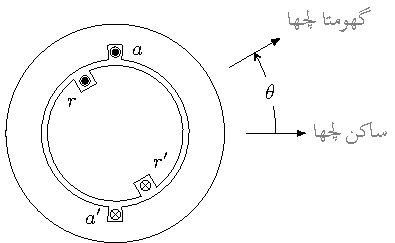
\includegraphics{figRotatingMachPrinciplesStatorAndRotorInductances}
\begin{tikzpicture}
%grid
%\draw[gray,thick] (-2*\sRo,-2*\sRo) grid (2*\sRo,3*\sRo);
%\draw[gray,thin,xstep=0.1,ystep=0.1] (-2*\sRo,-2*\sRo) grid (2*\sRo,3*\sRo);
%
\stator{2}{90}
\slotDot{90}
\slotCross{270}
\draw node at (90-15:\sRi+2*\gap){$a$};
\draw node at (-90-15:\sRi+2*\gap){$a'$};
%ROTOR
\pgfmathsetmacro{\pTheta}{165}
\pgfmathsetmacro{\pX}{0}
\pgfmathsetmacro{\pY}{0.25}
\pgfmathsetmacro{\rTilt}{30}
\rotor{2}{\rTilt}
%rotor dot
\draw (\rTilt+90:\rR-\delR/2) circle (2.5pt);
\draw[fill] (\rTilt+90:\rR-\delR/2) circle (1.5pt); 
%rotor cross
\draw (\rTilt-90:\rR-\delR/2) circle (2.5pt);
\draw (\rTilt-90:\rR-\delR/2)++(45:2.2pt)--++(-135:4.4pt);
\draw (\rTilt-90:\rR-\delR/2)++(-45:2.2pt)--++(135:4.4pt); 
%text
\draw node at (\rTilt+90+25:\rR-\pY){$r$};
\draw node at (\rTilt-90+30:\rR-\pY){$r'$};
%urdu
\draw[-latex] (0:1.2*\sRo)--++(0:1cm)node[right,gray]{\RL{ساکن لچھا}};
\draw[-latex] (\rTilt:1.2*\sRo)--++(\rTilt:1cm)node[above right,gray]{\RL{گھومتا لچھا}};
\draw[-stealth] (0:1.2*\sRo cm+0.5 cm) arc (0:\rTilt:1.2*\sRo cm+0.5 cm);
\draw  node[fill=white] at (\rTilt/2:1.2*\sRo cm+0.5 cm){$\theta$};
\end{tikzpicture}
\caption{ساکن امالہ اور گھومتا امالہ۔}
\label{شکل_گھومتے_مشین_ساکن_گھومتا_امالہ}
\end{figure}

اس طرح ساکن لچھے کی امالہ \عددیء{L_{aa}} اور گھومے لچھے کی امالہ \عددیء{L_{rr}} مقررہ ہیں جبکہ ان کا مشترکہ امالہ \عددیء{L_{ar}(\theta)} زاویہ \عددیء{\theta} پر منحصر ہو گا۔ جب \عددیء{\theta=0} یا \عددیء{\theta=\mp 2\pi}  کے برابر ہو تو ایک لچھے کا سارا مقناطیسی بہاو دوسرے لچھے سے بھی گزرتا ہے۔ ایسے حالت میں ان کا مشترکہ امالہ زیادہ سے زیادہ ہو گا جسے \عددیء{L_{ar0}} لکھتے ہیں۔ جب  \عددیء{\theta=\mp 180\degree} ہو اس لمحہ ایک مرتبہ پھر ایک لچھے کا سارا مقناطیسی بہاو دوسرے لچھے سے بھی گزرتا ہے البتہ اس لمحہ اس کی سمت اُلٹ ہوتی ہے لہٰذا اب ان کا مشترکہ امالہ بھی منفی ہو گا یعنی \عددیء{-L_{ar0}} اور جب \عددیء{\theta=\mp 90\degree} ہو  تب ان کا مشترکہ امالہ صفر ہو گا۔ اگر ہم یہ ذہن میں رکھیں کہ خلائی درز میں  مقناطیسی بہاو سائن نما ہے تب
\begin{align}
L_{ar}=L_{ar0} \cos \theta
\end{align}
ہو گا۔ہم ساکن اور گھومتے لچھوں کی ارتباط بہاو کو یوں لکھ سکتے ہیں
\begin{gather}
\begin{aligned}
\lambda_a&=L_{aa} i_a+L_{ar}(\theta) i_r=L_{aa} i_a+L_{ar0} \cos (\theta) i_r\\
\lambda_r&=L_{ar}(\theta) i_a+L_{rr} i_r=L_{ar0} \cos (\theta) i_a+L_{rr} i_r
\end{aligned}
\end{gather}
اگر ساکن لچھے کی مزاحمت \عددیء{R_a} اور گھومتے لچھے کی مزاحمت \عددیء{R_r} ہو تو ہم ان لچھوں کے سروں پر دیئے گئے برقی دباو کو یوں لکھ سکتے ہیں۔
\begin{gather}
\begin{aligned}
v_a&=i_a R_a +\frac{\dif \lambda_a}{\dif t}=i_a R_a+L_{aa} \frac{\dif i_a}{\dif t}+L_{ar0} \cos \theta \frac{\dif i_r}{\dif t}-L_{ar0}  i_r \sin \theta  \frac{\dif \theta}{\dif t}\\
v_r&=i_r R_r +\frac{\dif \lambda_r}{\dif t}=i_r R_r+L_{ar0} \cos \theta \frac{\dif i_a}{\dif t}-L_{ar0} i_a \sin \theta  \frac{\dif \theta}{\dif t}+L_{rr} \frac{\dif i_r}{\dif t}
\end{aligned}
\end{gather}
یہاں \عددیء{\theta} برقی زاویہ ہے اور وقت کے ساتھ اس کی تبدیلی رفتار \عددیء{\omega} کو ظاہر کرتی ہے یعنی
\begin{align}
\frac{\dif \theta}{\dif t}=\omega
\end{align}
میکانی قوت مروڑ بذریعہ کو توانائی حاصل کی جا سکتی ہے۔ کو توانائی صفحہ \حوالہصفحہ{مساوات_تبادلہ_کوتوانائی_از_خود} پر مساوات \حوالہ{مساوات_تبادلہ_کوتوانائی_از_خود}  سے حاصل ہوتی ہے۔ یہ مساوات موجودہ استعمال کے لئے یوں لکھا جا سکتا ہے۔
\begin{align}
W_m'=\frac{1}{2} L_{aa} i_a^2+\frac{1}{2} L_{rr} i_r^2+L_{ar0} i_a i_r \cos \theta
\end{align}
اس سے میکانی قوت مروڑ \عددیء{T_m} یوں حاصل ہوتا ہے۔
\begin{align}\label{مساوات_گھومتے_مشین_مروڑ_بذریعہ_توانائی}
T_m=\frac{\partial W_m'(\theta_m,i_a,i_r)}{\partial \theta_m}=\frac{\partial W_m'(\theta,i_a,i_r)}{\partial \theta} \frac{\partial \theta}{\partial \theta_m}
\end{align}
چونکہ \عددیء{P} قطب مشینوں کے لئے
\begin{align}
\theta=\frac{P}{2} \theta_m
\end{align}
لہٰذا ہمیں مساوات \حوالہ{مساوات_گھومتے_مشین_مروڑ_بذریعہ_توانائی}  سے ملتا ہے
\begin{align}\label{مساوات_گھومتے_مشین_مروڑ_بذریعہ_کوتوانائی}
T_m=-\frac{P}{2} L_{ar0} i_a i_r \sin \left(\frac{P}{2} \theta_m\right)
\end{align}
اس مساوات میں قوت مروڑ \عددیء{T_m} منفی ہے۔ اس کا مطلب ہے کہ اگر کسی لمحہ پر ساکن اور گھومتے لچھوں کے مقناطیسی بہاو کے درمیان زاویہ مثبت ہو تو ان کے مابین قوت مروڑ منفی ہو گا یعنی قوت مروڑ ان دونوں مقناطیسی بہاو کو ایک سمت میں رکھنے کی کوشش کرے گا۔

\جزوحصہ{مقناطیسی بہاو سے میکانی قوت مروڑ کا حساب}
شکل \حوالہ{شکل_گھومتے_مشین_لچھوں_کی_قطبین}  میں دو قطب والی ایک دور کی مشین دکھائی گئی ہے۔ اس شکل میں بائیں جانب صرف گھومتے لچھے میں برقی رو ہے۔ اس لچھے کا مقناطیسی بہاو تیر کے نشان سے دکھایا گیا ہے، یعنی تیر اس مقناطیس کے محور کو ظاہر کرتا ہے۔ یہاں اگر صرف گھومتے حصے پر توجہ دی جائے تو یہ واضح ہے کہ گھومتا حصہ ایک مقناطیس کی مانند ہے جس کے شمالی اور جنوبی قطبین شکل میں دیئے گئے ہیں۔ اسی طرح شکل میں دائیں جانب صرف ساکن لچھے میں برقی رو ہے۔ اگر اس مرتبہ صرف ساکن حصے پر توجہ دی جائے تو اس کے بائیں جانب سے مقناطیسی بہاو نکل کر خلائی درز میں داخل ہوتی ہے، لہٰذا یہی اس کا شمالی قطب ہے اور اس مقناطیس کا محور بھی اسی تیر کی سمت میں ہے۔
\begin{figure}
\centering
%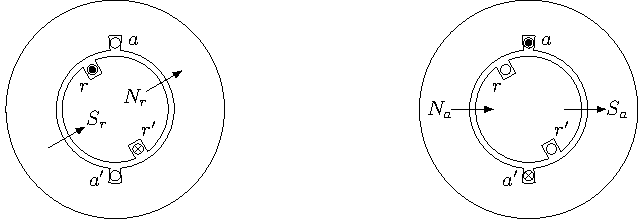
\includegraphics{figRotatingMachPrinciplesStatorAndRotorMagneticPoles}
\begin{tikzpicture}
%grid
%\draw[gray,thick] (-2*\sRo,-2*\sRo) grid (2*\sRo,3*\sRo);
%\draw[gray,thin,xstep=0.1,ystep=0.1] (-2*\sRo,-2*\sRo) grid (2*\sRo,3*\sRo);
%
\pgfmathsetmacro{\sRi}{0.8*\sRi}
\pgfmathsetmacro{\rR}{\sRi-\gap}

\stator{2}{90}
\slotDot{90}
\slotCross{270}
\draw node at (90-15:\sRi+2*\gap){$a$};
\draw node at (-90-15:\sRi+2*\gap){$a'$};
%
\draw[-latex] (0:\rR cm-0.3 cm)--++(0:0.7cm)node[xshift=0.2cm]{$S_a$};
\draw[latex-] (180:\rR cm-0.3 cm)--++(180:0.7cm)node[xshift=-0.2cm]{$N_a$};
%ROTOR
\pgfmathsetmacro{\pTheta}{165}
\pgfmathsetmacro{\pX}{0}
\pgfmathsetmacro{\pY}{0.25}
\pgfmathsetmacro{\rTilt}{30}
\rotor{2}{\rTilt}
%rotor no current
\draw (\rTilt+90:\rR-\delR/2) circle (2.5pt);
\draw (\rTilt-90:\rR-\delR/2) circle (2.5pt);
%text
\draw node at (\rTilt+90+25:\rR-\pY){$r$};
\draw node at (\rTilt-90+30:\rR-\pY){$r'$};
%
\begin{scope}[xshift=-7cm]
\stator{2}{90}
\slotEmptyCircle{90}
\slotEmptyCircle{270}
\draw node at (90-15:\sRi+2*\gap){$a$};
\draw node at (-90-15:\sRi+2*\gap){$a'$};
%
%ROTOR
\pgfmathsetmacro{\pTheta}{165}
\pgfmathsetmacro{\pX}{0}
\pgfmathsetmacro{\pY}{0.25}
\pgfmathsetmacro{\rTilt}{30}
\rotor{2}{\rTilt}
%rotor dot
\draw (\rTilt+90:\rR-\delR/2) circle (2.5pt);
\draw[fill] (\rTilt+90:\rR-\delR/2) circle (1.5pt); 
%rotor cross
\draw (\rTilt-90:\rR-\delR/2) circle (2.5pt);
\draw (\rTilt-90:\rR-\delR/2)++(45:2.2pt)--++(-135:4.4pt);
\draw (\rTilt-90:\rR-\delR/2)++(-45:2.2pt)--++(135:4.4pt); 
%
\draw[-latex] (\rTilt:\rR cm-0.3 cm)node[shift={(180+\rTilt:0.2cm)}]{$N_r$}--++(\rTilt:0.7cm);
\draw[latex-] (180+\rTilt:\rR cm-0.3 cm)node[shift={(\rTilt:0.25cm)}]{$S_r$}--++(180+\rTilt:0.7cm);
%text)
\draw node at (\rTilt+90+25:\rR-\pY){$r$};
\draw node at (\rTilt-90+30:\rR-\pY){$r'$};
\end{scope}
\end{tikzpicture}
\caption{لچھوں کے قطبین۔}
\label{شکل_گھومتے_مشین_لچھوں_کی_قطبین}
\end{figure}

یہاں یہ واضح رہے کہ اگرچہ گچھ لچھے دکھائے گئے ہیں  لیکن درحقیقت دونوں لچھوں کے مقناطیسی دباو سائن-نما ہی ہیں اور تیر کے نشان ان مقناطیسی دباو کی موج کے چوٹی کو ظاہر کرتے ہیں۔

شکل \حوالہ{شکل_گھومتے_مشین_خلائی_درز_مجموعی_دباو}  میں اب دونوں لچھوں میں برقی رو ہے۔ یہ واضح ہے کہ یہ بالکل دو مقناطیسوں کی طرح ہے اور ان کے اُلٹ قطبین کے مابین قوتِ کشش ہو گا، یعنی یہ دونوں لچھے ایک ہی سمت میں ہونے کی کوشش کریں گے۔
\begin{figure}
\centering
%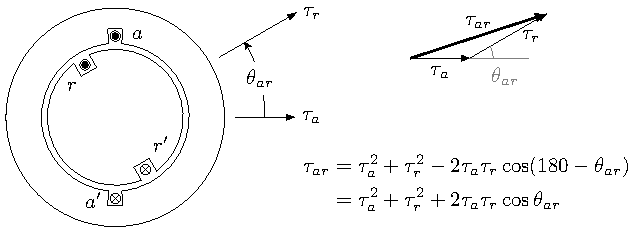
\includegraphics{figRotatingMachPrinciplesCombinedStatorAndRotorMMF}
\begin{tikzpicture}
%grid
%\draw[gray,thick] (-2*\sRo,-2*\sRo) grid (2*\sRo,3*\sRo);
%\draw[gray,thin,xstep=0.1,ystep=0.1] (-2*\sRo,-2*\sRo) grid (2*\sRo,3*\sRo);
%
\stator{2}{90}
\slotDot{90}
\slotCross{270}
\draw node at (90-15:\sRi+2*\gap){$a$};
\draw node at (-90-15:\sRi+2*\gap){$a'$};
%
%ROTOR
\pgfmathsetmacro{\pTheta}{165}
\pgfmathsetmacro{\pX}{0}
\pgfmathsetmacro{\pY}{0.25}
\pgfmathsetmacro{\rTilt}{30}
\rotor{2}{\rTilt}
%rotor dot
\draw (\rTilt+90:\rR-\delR/2) circle (2.5pt);
\draw[fill] (\rTilt+90:\rR-\delR/2) circle (1.5pt); 
%rotor cross
\draw (\rTilt-90:\rR-\delR/2) circle (2.5pt);
\draw (\rTilt-90:\rR-\delR/2)++(45:2.2pt)--++(-135:4.4pt);
\draw (\rTilt-90:\rR-\delR/2)++(-45:2.2pt)--++(135:4.4pt); 
%text
\draw node at (\rTilt+90+25:\rR-\pY){$r$};
\draw node at (\rTilt-90+30:\rR-\pY){$r'$};
%
\draw[-latex](0:1.1*\sRo)--++(0:1cm)node[right]{$\tau_a$};
\draw[-latex](\rTilt:1.1*\sRo)--++(\rTilt:1.5cm)node[right]{$\tau_r$};
\draw[-stealth] (0:1.1*\sRo cm+0.5cm) arc (0:\rTilt:1.1*\sRo cm +0.5 cm);
\draw node[fill=white] at (\rTilt/2:1.1*\sRo cm+0.5 cm){$\theta_{ar}$};
%text
\draw (3 cm,-0.5 cm) node[below right] {$
\begin{aligned}
\tau_{ar}&=\tau_a^2+\tau_r^2-2 \tau_a \tau_r \cos (180-\theta_{ar})\\
&=\tau_a^2+\tau_r^2+2 \tau_a \tau_r \cos \theta_{ar}
\end{aligned}
$};
%
\begin{scope}[xshift=5 cm,yshift=1cm]
\draw[-latex] (0,0)--++(0:1 cm)coordinate(aTip)node[below,pos=0.5]{$\tau_a$};
\draw[-latex] (aTip)--++(\rTilt:1.5 cm)coordinate(rTip)node[below,pos=0.8]{$\tau_r$};
\draw[-latex,thick](0,0)--(rTip)node[above,pos=0.5]{$\tau_{ar}$};
%angle
\draw[gray](aTip)--++(1cm,0);
\draw[gray](aTip)++(0.4cm,0)node[shift={(0.2cm,-0.3cm)}]{$\theta_{ar}$} arc (0:\rTilt:0.4 cm);
\end{scope}
\end{tikzpicture}
\caption{خلائی درز میں مجموعی مقناطیسی دباو۔}
\label{شکل_گھومتے_مشین_خلائی_درز_مجموعی_دباو}
\end{figure}

یہاں یہ زیادہ واضح ہے کہ یہ دو مقناطیس کوشش کریں گے کہ \عددیء{\theta_{ar}} صفر کے برابر ہو یعنی ان کا میکانی قوت مروڑ \عددیء{\theta_{ar}} کے اُلٹ سمت میں ہو گا۔ یہی کچھ مساوات \حوالہ{مساوات_گھومتے_مشین_مروڑ_بذریعہ_کوتوانائی}  کہتا ہے ۔

ان برقی مقناطیسوں کے مقناطیسی دباو کو اگر ان کے مقناطیسی محور کی سمت میں \عددیء{\سمتیہ{\tau}_a} اور \عددیء{\سمتیہ{\tau}_r} سے ظاہر کیا جائے جہاں \عددیء{\tau_a} اور \عددیء{\tau_r} مقناطیسی دباو کے چوٹی کے برابر ہوں تو خلاء میں کُل مقناطیسی دباو \عددیء{\سمتیہ{\tau}_{ar}} ان  کا جمع سمتیات ہو گا جیسے شکل میں دکھایا گیا ہے۔ اس کا طول \عددیء{\tau_{ar}} کوسائن کے قلیہ\حاشیہب{cosine law}  سے یوں حاصل ہوتا ہے۔
\begin{gather}
\begin{aligned}\label{مساوات_گھومتے_مشین_مربع_کل_دباو}
\tau_{ar}^2&=\tau_a^2+\tau_r^2-2\tau_a \tau_r \cos (180\degree-\theta_{ar})\\
&=\tau_a^2+\tau_r^2+2\tau_a \tau_r \cos \theta_{ar}
\end{aligned}
\end{gather}
خلائی درز میں یہ کُل مقناطیسی دباو، مقناطیسی شدت \عددیء{H_{ar}} کو جنم دے گا جو اس قلیہ سے حاصل ہوتا ہے۔
\begin{align}
\tau_{ar}=H_{ar} l_g
\end{align}
\عددیء{H_{ar}} مقناطیسی شدت کی چوٹی کو ظاہر کرتا ہے۔ اب جہاں خلاء میں مقناطیسی شدت \عددیء{H} ہو وہاں مقناطیسی ہمہ توانائی کی کثافت \عددیء{\tfrac{\mu_0}{2}H^2} ہوتی ہے۔ خلائی درز میں اوسط ہمہ توانائی کی کثافت اس خلائی درز میں \عددیء{H^2} کی اوسط ضربِ \عددیء{\tfrac{\mu_0}{2}} ہو گی۔ کسی بھی سائن نما موج \عددیء{H=H_0 \cos \theta} کے \عددیء{H^2} کا اوسط \عددیء{H_{\textup{اوسط}}^2} یوں حاصل کیا جاتا ہے۔
\begin{gather}
\begin{aligned}
H_{\textup{اوسط}}^2&=\frac{1}{\pi} \int_{-\frac{\pi}{2}}^{+\frac{\pi}{2}} H^2 \dif \theta\\
&=\frac{1}{\pi} \int_{-\frac{\pi}{2}}^{+\frac{\pi}{2}} H_0^2 \cos^2 \theta \dif \theta\\
&=\frac{H_0^2}{\pi} \int_{-\frac{\pi}{2}}^{+\frac{\pi}{2}} \frac{1+\cos 2 \theta}{2} \dif \theta\\
&=\frac{H_0^2}{\pi}  \left.  \frac{\theta +\frac{\sin 2 \theta}{2}}{2} \right|_{-\frac{\pi}{2}}^{+\frac{\pi}{2}}\\
&=\frac{H_0^2}{2}
\end{aligned}
\end{gather}
لہٰذا خلائی درز میں اوسط ہمہ توانائی کی کثافت \عددیء{\tfrac{\mu_0}{2}\tfrac{H_{ar}^2}{2}} ہو گی اور اس خلاء میں کُل ہمہ توانائی اس اوسط ہمہ توانائی ضربِ خلاء کی حجم کے برابر ہو گا یعنی
\begin{align}
W_m'=\frac{\mu_0}{2} \frac{H_{ar}^2}{2} 2 \pi r l_g l=\frac{\mu_0 \pi r l}{2l_g} \tau_{ar}^2
\end{align}
اس مساوات میں خلائی درز کی رداسی لمبائی \عددیء{l_g} ہے اور اس کی دھرے\حاشیہب{axis} کی سمت میں محوری لمبائی\حاشیہب{axial length} \عددیء{l} ہے۔ محور سے خلاء کی اوسط رداسی فاصلہ \عددیء{r} ہے۔ مزید یہ کہ \عددیء{r\gg l_g} ہے۔ اس طرح خلاء میں رداسی سمت میں کثافتِ مقناطیسی بہاو کی تبدیلی کو نظر انداز کیا جا سکتا ہے۔ اس مساوات کو ہم مساوات \حوالہ{مساوات_گھومتے_مشین_مربع_کل_دباو}  کی مدد سے یوں لکھ سکتے ہیں۔
\begin{align}
W_m'=\frac{\mu_0 \pi r l}{2 l_g} \left(\tau_a^2+\tau_r^2+2\tau_a \tau_r \cos \theta_{ar} \right) 
\end{align}
اس سے میکانی قوت مروڑ یوں حاصل کیا جا سکتا ہے
\begin{align}\label{مساوات_گھومتے_مشین_مروڑ_کوتوانائی_سے}
T_m=\frac{\partial W_m'}{\partial \theta_{ar}}=-\frac{\mu_0 \pi r l}{l_g} \tau_a \tau_r \sin \theta_{ar}
\end{align}
یہ حساب دو قطب والی مشین کے لئے لگایا گیا ہے۔\عددیء{P} قطب والے مشین کے لئے یہ مساوات ہر جوڑی قطب کا میکانی قوت مروڑ دیتا ہے لہٰذا ایسے مشین کے لئے ہم لکھ سکتے ہیں
\begin{align}\label{مساوات_گھومتے_مشین_مروڑ_بذریعہ_کوتوانائی_الف}
T_m=-\frac{P}{2}\frac{\mu_0 \pi r l}{l_g} \tau_a \tau_r \sin \theta_{ar}
\end{align}
یہ ایک بہت اہم مساوات ہے۔ اس کے مطابق مشین کا میکانی قوت مروڑ اس کے ساکن اور گھومتے لچھوں کے مقناطیسی دباو کے چوٹی کے براہ راست متناسب ہے۔ اسی طرح یہ ان دونوں کے درمیان برقی زاویہ \عددیء{\theta_{ar}} کے سائن کے بھی براہ راست متناسب ہے۔ منفی میکانی قوت مروڑ کا مطلب ہے کہ یہ زاویہ  \عددیء{\theta_{ar}} کے الٹ جانب ہے یعنی یہ میکانی قوت مروڑ اس زاویہ کو کم کرنے کی جانب کو ہے۔ مشین کے ساکن اور گھومتے حصوں پر ایک برابر مگر الٹ سمتوں میں میکانی قوت مروڑ ہوتا ہے البتہ ساکن حصے کا قوت مروڑ مشین کے وجود کے ذریعہ زمین تک منتقل ہو جاتا ہے جبکہ گھومتے حصے کا میکانی قوت مروڑ اس حصے کو گھماتا ہے۔

چونکہ مقناطیسی دباو برقی رو کے براہ راست متناسب ہے لہٰذا  \عددیء{\tau_a} اور \عددیء{i_a} آپس میں براہ راست متناسب ہیں جبکہ \عددیء{\tau_r} اور \عددیء{i_r} آپس میں براہ راست متناسب ہیں۔ اس سے یہ ظاہر ہوتا ہے کہ مساوات \حوالہ{مساوات_گھومتے_مشین_مروڑ_بذریعہ_کوتوانائی}  اور \حوالہ{مساوات_گھومتے_مشین_مروڑ_بذریعہ_کوتوانائی_الف}  ایک جیسے ہیں۔ درحقیقت یہ ثابت کیا جا سکتا ہے کہ یہ دونوں بالکل برابر ہیں۔

شکل \حوالہ{شکل_گھومتے_مشین_بہاو_کے_زاویے}  میں ایک مرتبہ پھر ساکن اور گھومتے لچھوں کے مقناطیسی دباو دکھائے گئے ہیں۔ شکل میں بائیں جانب تکون \عددیء{\Delta AEC} اور \عددیء{\Delta BEC} میں \عددیء{CE} مشترکہ ہے اور ان دو تکونوں سے واضح ہے کہ
\begin{align}
CE=\tau_r \sin \theta_{ar}=\tau_{ar} \sin \theta_a
\end{align}
اس مساوات کی مدد سے مساوات \حوالہ{مساوات_گھومتے_مشین_مروڑ_بذریعہ_کوتوانائی_الف}  یوں لکھا جا سکتا ہے۔
\begin{align}\label{مساوات_گھومتے_مشین_مروڑ_بذریعہ_کوتوانائی_ب}
T_m=-\frac{P}{2}\frac{\mu_0 \pi r l}{l_g} \tau_a \tau_{ar}  \sin \theta_a
\end{align}
%
\begin{figure}
\centering
%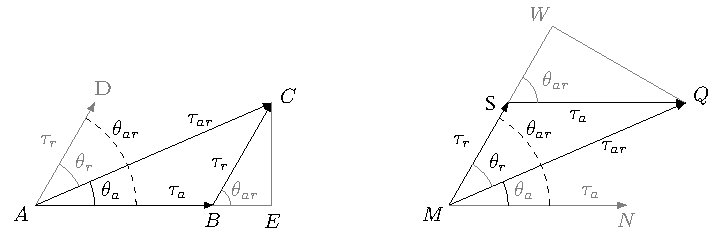
\includegraphics{figRotatingMachPrinciplesFluxAngles}
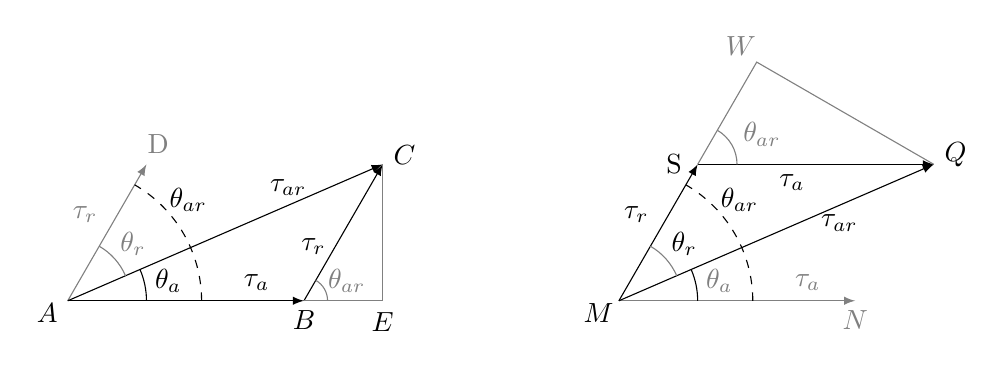
\begin{tikzpicture}
%grid
%\draw[gray,thick] (-2*\sRo,-2*\sRo) grid (2*\sRo,3*\sRo);
%\draw[gray,thin,xstep=0.1,ystep=0.1] (-2*\sRo,-2*\sRo) grid (2*\sRo,3*\sRo);
%
\draw[-latex](0,0)node[shift={(210:0.3cm)}]{$A$}--++(0:3 cm)coordinate(aTip)node[above,pos=0.8]{$\tau_a$}node[below]{$B$};
\draw[gray,-latex](0,0)--++(60:2 cm)node[above left,pos=0.5]{$\tau_r$}node[shift={(60:0.3 cm)}]{D};
\draw[-latex](aTip)--++(60:2cm)coordinate(rTip)node[left,pos=0.4]{$\tau_r$};
\draw[-latex](0,0)--(rTip)node[above,pos=0.7]{$\tau_{ar}$}node[shift={(23:0.3cm)}]{$C$}node[yshift=-2cm]{$E$};
\draw[gray](aTip)-|(rTip);
\draw[gray](aTip)++(0.3,0) arc (0:60:0.3 cm);
\draw[gray] (aTip)++(25:0.6 cm) node{$\theta_{ar}$};
%angles
\draw(0:1 cm) arc (0:23.413:1 cm);
\draw (11:1.3 cm) node{$\theta_{a}$};
%
\draw[gray](23.413:0.8 cm) arc (23.413:60:0.8 cm);
\draw[gray] (41:1.1 cm) node{$\theta_{r}$};
%
\draw[dashed](0:1.7 cm) arc (0:60:1.7cm);
\draw (40:2cm) node{$\theta_{ar}$};
%========
\begin{scope}[xshift=7cm]
\draw[gray,-latex](0,0)node[black,shift={(210:0.3cm)}]{$M$}--++(0:3 cm)coordinate(aTip)node[gray,above,pos=0.8]{$\tau_a$}node[below]{$N$};
\draw[-latex](0,0)--++(60:2 cm)node[above left,pos=0.5]{$\tau_r$}coordinate(rTipR)node[shift={(180:0.3 cm)}]{S};
\draw[-latex](rTipR)--++(0:3 cm)coordinate(aTip)node[below,pos=0.4]{$\tau_a$};
\draw[-latex](0,0)--(aTip)node[below,pos=0.7]{$\tau_{ar}$}node[shift={(23:0.3cm)}]{$Q$};
\draw[gray](rTipR)--++(60:1.5 cm)node[shift={(-0.2,0.2)}]{$W$}--(aTip);
%angles
\draw(0:1 cm) arc (0:23.413:1 cm);
\draw (11:1.3 cm) node[gray]{$\theta_{a}$};
%
\draw[gray](23.413:0.8 cm) arc (23.413:60:0.8 cm);
\draw (41:1.1 cm) node{$\theta_{r}$};
%
\draw[dashed](0:1.7 cm) arc (0:60:1.7cm);
\draw (40:2cm) node{$\theta_{ar}$};
%
\draw[gray](rTipR)++(0.5,0) arc (0:60:0.5);
\draw[gray](rTipR)++(25:0.9)node{$\theta_{ar}$};
\end{scope}
\end{tikzpicture}
\caption{مقناطیسی بہاو اور ان کے زاویے۔}
\label{شکل_گھومتے_مشین_بہاو_کے_زاویے}
\end{figure}
اسی طرح شکل \حوالہ{شکل_گھومتے_مشین_بہاو_کے_زاویے}  کے دائیں جانب تکون \عددیء{\Delta MWQ} اور تکون \عددیء{\Delta SWQ} میں \عددیء{WQ} کا طرف مشترکہ ہے اور ان دو تکونوں سے واضح ہے کہ
\begin{align}
WQ=\tau_a \sin \theta_{ar}=\tau_{ar} \sin \theta_r
\end{align}
اب اس مساوات کی مدد سے مساوات \حوالہ{مساوات_گھومتے_مشین_مروڑ_بذریعہ_کوتوانائی_الف}  یوں لکھا جا سکتا ہے۔
\begin{align}\label{مساوات_گھومتے_مشین_مروڑ_بذریعہ_کوتوانائی_پ}
T_m=-\frac{P}{2}\frac{\mu_0 \pi r l}{l_g} \tau_r \tau_{ar}  \sin \theta_r
\end{align}
مساوات \حوالہ{مساوات_گھومتے_مشین_مروڑ_بذریعہ_کوتوانائی_الف}  مساوات \حوالہ{مساوات_گھومتے_مشین_مروڑ_بذریعہ_کوتوانائی_ب}  اور مساوات \حوالہ{مساوات_گھومتے_مشین_مروڑ_بذریعہ_کوتوانائی_پ}  کو ایک جگہ لکھتے ہیں۔
\begin{gather}
\begin{aligned}\label{مساوات_گھومتے_مشین_مروڑ_بذریعہ_کوتوانائی_ت}
T_m&=-\frac{P}{2}\frac{\mu_0 \pi r l}{l_g} \tau_a \tau_r \sin \theta_{ar}\\
T_m&=-\frac{P}{2}\frac{\mu_0 \pi r l}{l_g} \tau_a \tau_{ar}  \sin \theta_a\\
T_m&=-\frac{P}{2}\frac{\mu_0 \pi r l}{l_g} \tau_r \tau_{ar}  \sin \theta_r
\end{aligned}
\end{gather}
ان مساوات سے یہ واضح ہے کہ میکانی قوت مروڑ کو دونوں لچھوں کے مقناطیسی دباو اور ان کے مابین زاویہ کی شکل میں لکھا جا سکتا ہے یا پھر ایک لچھے کی مقناطیسی دباو اور کُل مقناطیسی دباو اور ان دو کے مابین زاویہ کی شکل میں لکھا جا سکتا ہے۔

اس بات کو یوں بیان کیا جاسکتا ہے کہ میکانی قوت مروڑ دو مقناطیسی دباو کے آپس میں ردعمل کی وجہ سے وجود میں آتا ہے اور یہ ان مقناطیسی دباو کی چوٹی اور ان کے مابین زاویہ پر منحصر ہوتا ہے۔

مقناطیسی دباو، مقناطیسی شدت، کثافت مقناطیسی بہاو اور مقناطیسی بہاو سب کا آپس میں تعلق رکھتے ہیں لہٰذا ان مساوات کو کئی مختلف طریقوں سے لکھا جا سکتا ہے۔ مثلاً خلائی درز میں کُل مقناطیسی دباو \عددیء{\tau_{ar}} اور  وہاں کثافت مقناطیسی بہاو \عددیء{B_{ar}} کا تعلق
\begin{align}
B_{ar}=\frac{\mu_0 \tau_{ar}}{l_g}
\end{align}
استعمال کر کے مساوات \حوالہ{مساوات_گھومتے_مشین_مروڑ_بذریعہ_کوتوانائی_ت}  کے آخری جزو کو یوں لکھا جا سکتا ہے
\begin{align}
T_m=-\frac{P}{2} \pi r l \tau_r B_{ar} \sin \theta_r
\end{align}
مقناطیسی آلوں میں مقناطیسی قالب کی مقناطیسی مستقل \عددیء{\mu}  کی محدود صلاحیت کی وجہ سے قالب میں کثافت مقناطیسی بہاو تقریباً ایک ٹسلا تک ہی بڑھائی جا سکتی ہے۔ لہٰذا مشین بناتے وقت اس حد کو مد نظر رکھنا پڑتا ہے۔ اسی طرح گھومتے لچھے کا مقناطیسی دباو اس لچھے میں برقی رو پر منحصر ہوتا ہے۔ اس برقی رو سے لچھے کی مزاحمت میں برقی توانائی ضائع ہوتی ہے جس سے یہ لچھا گرم ہوتا ہے۔ برقی رو کو اس حد تک بڑھایا جا سکتا ہے جہاں تک اس لچھے کو ٹھنڈا کرنا ممکن ہو۔ لہٰذا مقناطیسی دباو کو اس حد کے اندر رکھنا پڑتا ہے۔ چونکہ اس مساوات میں یہ دو بہت ضروری حدیں واضح طور پر سامنے ہیں اس لئے یہ مساوات مشین بنانے کی غرض سے بہت اہم ہے۔

اس مساوات کی ایک اور بہت اہم شکل اب دیکھتے ہیں۔ ایک قطب پر مقناطیسی بہاو \عددیء{\phi_P}  ایک قطب پر اوسط کثافت مقناطیسی بہاو \عددیء{B_{\textup{اوسط}}} ضربِ ایک قطب کا رقبہ  \عددیء{A_P} ہوتا ہے۔ جہاں
\begin{align}
B_{\textup{اوسط}}&=\frac{1}{\pi} \int_{-\frac{\pi}{2}}^{+\frac{\pi}{2}} B_0 \cos \theta \dif \theta=\frac{2 B_0}{\pi}\\
A_P&=\frac{2\pi rl}{P}
\end{align}
لہٰذا
\begin{align}
\phi_P=\frac{2 B_0}{\pi}\frac{2\pi rl}{P}
\end{align}
اور
\begin{align}\label{مساوات_گھومتے_مشین_مروڑ_اور_بہاو}
T_m=-\frac{\pi}{2} \left(\frac{P}{2} \right)^2 \phi_{ar} \tau_r \sin \theta_r
\end{align}
یہ مساوات معاصر مشینوں  کے لئے بہت کار آمد ہے۔
